%%%%%%%%%%%%%%%%%%%%%%%%%%%%%%%%%%%%%%%%%%%%%%%%%%%%%%%%%%%%%%%%%%%%
%%%%%%%%%%%%%%%%%%%%%%%%%%%%%%%%%%%%%%%%%%%%%%%%%%%%%%%%%%%%%%%%%%%%
%%%%%%%%%%%%%%%%%%%%%%%%%%%%%%%%%%%%%%%%%%%%%%%%%%%%%%%%%%%%%%%%%%%%
%%%%%%%%%%%%%%%%%%%%%%%%%%%%%%%%%%%%%%%%%%%%%%%%%%%%%%%%%%%%%%%%%%%%%%%%%%
%We perform a likelihood fit of the $m_{jj}$ distribution for the electron 
%and muon samples combined (and also separately for each as cross check).
%The fit is performed in the $m_{jj}$ region [30,250] GeV and estimates the 
%fractions of diboson, W+jets, QCD, and top backgrounds using $m_{jj}$ 
%templates obtained from the CMS full simulation. 
%The total diboson and W+jets contribution are free parameters of the fit,
%while top and single top contribution are constrained to the measured 
%cross section. 
%The QCD multi-jet background is insignificant; however, we plan to 
%constrain its contribution by performing a fit to the the $\met$ distribution. 
%This simple method allows to search for a signal peak over a smooth background.
%
%
%Finally, we plot the $m_{jj}$ distribution in data after subtracting all 
%background components except diboson. 
%The diboson peak is prominently visible in this peak. 
%We then examine the $120--160~\gev$ mass range for any additional 
%excess. 
%We also overlay predictions of several new physics models described in 
%section~\ref{sec:NewPhysics}.
%
%%%%%%%%%%%%%%%%%%%%%%%%%%%%%%%%%%%%%%%%%%%%%%%%%%%%%%%%%%%%%%%%%%%%%%%%%%
%%%%%%%%%%%%%%%%%%%%%%%%%%%%%%%%%%%%%%%%%%%%%%%%%%%%%%%%%%%%%%%%%%%%%%%%%%
\clearpage{}
\section{Determination of yields from a fit to the \texorpdfstring{$m_{jj}$}{dijet invariant mass} distribution}
\label{sec:mjj_fit}
In order to set a limit on an anomalous resonance in the dijet mass spectrum, 
we first need to estimate the total yields of the various background 
components present in the data.
We extract the background yields from 
an unbinned maximum likelihood fit to the 
dijet invariant mass distribution $m_{jj}$,  
excluding the signal region (
$123~{\mbox{GeV}} < m_{jj} < 186~{\mbox{GeV}}$). 
Events in the signal region are later used 
to set exclusion limits. 
Table~\ref{tab:mjj_shapes_and_normalization} shows how the 
shape of each component is determined, and what constraints 
are applied to fit for the normalization; while the fit output 
is summarized in Tables~\ref{table:FitTotalsAndComparisons_mu} 
and \ref{table:FitTotalsAndComparisons_el}.
The main sources of 
systematics error are the uncertainties in the factorization 
and renormalization scales ($q^2$) and the matrix element -- parton shower 
matching scale in the the leading-order W+jets Monte Carlo, as well as 
the jet energy scale (JES) uncertainty. 
%%%%%%%%%%%%%%%
\begin{table}[!ht]
  \begin{center}
 \caption{Determination of the $m_{jj}$ shape and normalization.}  
 \label{tab:mjj_shapes_and_normalization} 
 \begin{tabular} {l  c  c c c }
   \hline \hline
   Process                &    Shape                         &  Shape syst.           & Normalization   &  Norm. syst.\\  \hline
   W+jets                 &    MC/ data                      &  $q^2$, matching, JES  & Unconstrained   &  Unconstrained \\
   diboson                &    MC                            &  JES                   & Constrain: NLO        &  Gauss $\sigma =10\%$ \\ 
   $t\bar{t}$ &    MC                            &  JES                   & Constrain: NLO        &  Gauss $\sigma =7\%$  \\ 
   single top & MC & JES & Constrain:NLO & Gauss $\sigma=5\%$ \\
   Z+jets                 &    MC                            &  JES                   & Constrain: NLO        &  Gauss $\sigma =4.3\%$  \\
   QCD                    &    data                          &  JES                   & Constrain: MET fit in data  &  Sec.~\ref{sec:qcd_Uncertainty}  \\\hline \hline
 \end{tabular}
\end{center}
\end{table}
%%%%%%%%%%%%%%%%%%%%%%%%%%%%%%%%%%%%%%%%%%%%%%%%%%%%%%%%%%%%%%%
%%%\begin{table}[!htbp]
%%%  \begin{center}
%%% \caption{Event yields determined from a likelihood fit
%%% to the data. The total uncertainty takes into
%%% account the correlations among individual components.}
%%% \label{tab:mjj_shapes_and_normalization}
%%% \begin{tabular} {l  c  c c c }
%%%   \hline \hline
%%%   Process             &    \multicolumn{2}{c}{Muon channel} & \multicolumn{2}{c}{Electron channel} \\  
%%%\hline
%%%                       &    2 jets              &  3 jets              & 2 jets             &  3 jets\\  
%%%\hline
%%%   W+jets              &    53231  $\pm$  466   &  12551 $\pm$  331    &  30075 $\pm$ 115   &  8725 $\pm$  273\\
%%%   Dibosons            &    1087 $\pm$  98      &  339 $\pm$  49       &  642 $\pm$  61     &  173 $\pm$  17\\
%%%   $t\bar{t}$          &    3973  $\pm$  238    &  7738 $\pm$  330     &  2313 $\pm$ 143    &  3939 $\pm$  216\\
%%%   Single top          &    1545  $\pm$  76     &  873 $\pm$  43       &  858 $\pm$  43     &  489 $\pm$  24\\
%%%   Drell-Yan+jets      &    1362 $\pm$  58      &  417 $\pm$  18       &  993 $\pm$  43     &  341 $\pm$  15\\
%%%   Multijet            &    84 $\pm$  256       &  0 $\pm$ 90          &  4040 $\pm$ 1170   &  334 $\pm$  160\\
%%%\hline
%%%   Total from fit      &    61281 $\pm$ 290     &  21918 $\pm$ 183     &  38923 $\pm$ 227   &  14000 $\pm$ 141\\
%%%   Data                &    61153               &  22030               &  38973             &  14145 \\
%%%\hline
%%%\multicolumn{5}{c}{in region $(123\,\text{GeV} < m_{jj} < 186\,\text{GeV})$} \\
%%%\hline
%%%  Total from fit & 12921 $\pm$ 118 & 7021 $\pm$ 91 & 7909 $\pm$ 92 & 4297 $\pm$ 70\\
%%%  Data & 12761 & 7111 & 8023 & 4438 \\
%%%\hline \hline
%%% \end{tabular}
%%%\end{center}
%%%\end{table}
%%%%%%%%%%%%%%%%%%%%%%%%%%%%%%%%%%%%%%%%%%%%%%%%%%%%%%%%%%%%%%%
\subsection{Fit results for the 2-jet sample}
\label{sec:mjj_2jetfit}
The results of the fit for the 2-jet sample are shown 
in Figs.~\ref{fig:mjj_2jet_mu} and~\ref{fig:mjj_2jet_el}. 
A clear peak from the Standard Model electroweak diboson 
WW/WZ production can be seen. 
The mean mass, resolution and yield for the diboson events are 
consistent with the Standard Model predictions computed up to 
the next-to-leading order (NLO) in perturbation theory.
Tese consistency checks give us confidence in the analysis procedures.
The fit results are tabulated below.
%%%%%%%%%%%%%%%%%%%%

Muons
{\footnotesize
\begin{verbatim}
 COVARIANCE MATRIX CALCULATED SUCCESSFULLY
 FCN=-257146 FROM HESSE     STATUS=OK             73 CALLS         289 TOTAL
                     EDM=2.73414e-06    STRATEGY= 1      ERROR MATRIX ACCURATE 
  EXT PARAMETER                                INTERNAL      INTERNAL  
  NO.   NAME      VALUE            ERROR       STEP SIZE       VALUE   
   1  fMU          2.47393e-01   7.83851e-02   1.88808e-02   2.49989e-01
   2  fSU         -9.96001e-02   6.60148e-02   1.50362e-02  -9.97655e-02
   3  nDiboson     1.23654e+03   1.14351e+02   3.61207e+01   1.23654e+03
   4  nQCD         2.92262e+01   2.84110e+02   7.26591e+01   2.92262e+01
   5  nSingleTop   1.76534e+03   8.72275e+01   2.94352e+01   1.76534e+03
   6  nTTbar       4.50689e+03   3.07076e+02   7.85635e+01   4.50689e+03
   7  nWjets       5.89188e+04   5.29563e+02   1.04637e+02   5.89188e+04
   8  nZjets       1.83714e+03   7.88493e+01   2.66628e+01   1.83714e+03
                               ERR DEF= 0.5
 EXTERNAL ERROR MATRIX.    NDIM=  25    NPAR=  8    ERR DEF=0.5
  6.158e-03  3.729e-03 -9.830e-01  3.397e-01 -1.737e-01 -1.688e+00  1.321e+00  4.026e-02 
  3.729e-03  4.364e-03 -1.153e+00  1.369e+00  6.222e-02  2.860e+00 -6.016e+00 -7.244e-02 
 -9.830e-01 -1.153e+00  1.308e+04  2.627e+02 -4.831e+01 -4.929e+02 -1.428e+04 -1.648e+01 
  3.397e-01  1.369e+00  2.627e+02  8.072e+04 -3.304e+01 -5.671e+02 -8.043e+04  2.022e-01 
 -1.737e-01  6.222e-02 -4.831e+01 -3.304e+01  7.609e+03 -2.188e+02 -7.003e+03 -1.503e+00 
 -1.688e+00  2.860e+00 -4.929e+02 -5.671e+02 -2.188e+02  9.430e+04 -8.492e+04 -9.974e+00 
  1.321e+00 -6.016e+00 -1.428e+04 -8.043e+04 -7.003e+03 -8.492e+04  2.804e+05 -6.144e+03 
  4.026e-02 -7.244e-02 -1.648e+01  2.022e-01 -1.503e+00 -9.974e+00 -6.144e+03  6.217e+03 
 PARAMETER  CORRELATION COEFFICIENTS  
       NO.  GLOBAL      1      2      3      4      5      6      7      8
        1  0.74609   1.000  0.719 -0.110  0.015 -0.025 -0.070  0.032  0.007
        2  0.76270   0.719  1.000 -0.153  0.073  0.011  0.141 -0.172 -0.014
        3  0.43099  -0.110 -0.153  1.000  0.008 -0.005 -0.014 -0.236 -0.002
        4  0.68207   0.015  0.073  0.008  1.000 -0.001 -0.006 -0.535  0.000
        5  0.26628  -0.025  0.011 -0.005 -0.001  1.000 -0.008 -0.152 -0.000
        6  0.68159  -0.070  0.141 -0.014 -0.006 -0.008  1.000 -0.522 -0.000
        7  0.82455   0.032 -0.172 -0.236 -0.535 -0.152 -0.522  1.000 -0.147
        8  0.25912   0.007 -0.014 -0.002  0.000 -0.000 -0.000 -0.147  1.000

  RooFitResult: minimized FCN value: -257146, estimated distance to minimum: 2.73414e-06
                covariance matrix quality: Full, accurate covariance matrix

    Floating Parameter  InitialValue    FinalValue +/-  Error     GblCorr.
  --------------------  ------------  --------------------------  --------
                   fMU    1.0000e-01    2.4739e-01 +/-  7.84e-02  <none>
                   fSU    3.0000e-01   -9.9600e-02 +/-  6.60e-02  <none>
              nDiboson    1.1500e+03    1.2365e+03 +/-  1.14e+02  <none>
                  nQCD    9.0000e+01    2.9226e+01 +/-  2.84e+02  <none>
            nSingleTop    1.4750e+03    1.7653e+03 +/-  8.72e+01  <none>
                nTTbar    3.7500e+03    4.5069e+03 +/-  3.07e+02  <none>
                nWjets    4.5000e+04    5.8919e+04 +/-  5.30e+02  <none>
                nZjets    1.2500e+03    1.8371e+03 +/-  7.88e+01  <none>

total yield: 68294 +/- 307
\end{verbatim}
}

Electrons
{\footnotesize
\begin{verbatim}
 COVARIANCE MATRIX CALCULATED SUCCESSFULLY
 FCN=-131188 FROM HESSE     STATUS=OK             61 CALLS         302 TOTAL
                     EDM=9.41539e-06    STRATEGY= 1      ERROR MATRIX ACCURATE 
  EXT PARAMETER                                INTERNAL      INTERNAL  
  NO.   NAME      VALUE            ERROR       STEP SIZE       VALUE   
   1  fMU         -5.36931e-02   5.28293e-02   2.45017e-03  -5.37189e-02
   2  fSU          3.34989e-01   7.04288e-02   6.87962e-04   3.41594e-01
   3  nDiboson     6.85068e+02   6.45681e+01   3.04971e+00   6.85068e+02
   4  nQCD         3.94395e+03   1.13294e+03   2.22700e+00   3.94395e+03
   5  nSingleTop   9.15639e+02   4.61301e+01   2.26577e+00   9.15639e+02
   6  nTTbar       2.55566e+03   1.73993e+02   7.17593e+00   2.55566e+03
   7  nWjets       2.97871e+04   1.15263e+03   2.25105e+00   2.97871e+04
   8  nZjets       1.06150e+03   4.55915e+01   2.23263e+00   1.06150e+03
                               ERR DEF= 0.5
 EXTERNAL ERROR MATRIX.    NDIM=  25    NPAR=  8    ERR DEF=0.5
  2.794e-03  1.310e-03 -1.914e-02  5.589e+00  2.502e-02  6.957e-01 -7.018e+00 -2.181e-02 
  1.310e-03  4.969e-03  2.986e-01  1.000e+01 -5.746e-02 -1.214e+00 -9.815e+00  1.933e-02 
 -1.914e-02  2.986e-01  4.169e+03 -4.048e+03 -1.233e+01 -9.034e+01 -7.755e+02 -6.162e+00 
  5.589e+00  1.000e+01 -4.048e+03  1.284e+06 -6.401e+02 -3.606e+03 -1.264e+06 -4.856e+02 
  2.502e-02 -5.746e-02 -1.233e+01 -6.401e+02  2.128e+03 -5.221e+01 -1.289e+03 -1.108e-01 
  6.957e-01 -1.214e+00 -9.034e+01 -3.606e+03 -5.221e+01  3.027e+04 -2.257e+04  9.884e+00 
 -7.018e+00 -9.815e+00 -7.755e+02 -1.264e+06 -1.289e+03 -2.257e+04  1.329e+06 -1.645e+03 
 -2.181e-02  1.933e-02 -6.162e+00 -4.856e+02 -1.108e-01  9.884e+00 -1.645e+03  2.079e+03 
 PARAMETER  CORRELATION COEFFICIENTS  
       NO.  GLOBAL      1      2      3      4      5      6      7      8
        1  0.37831   1.000  0.351 -0.006  0.093  0.010  0.076 -0.115 -0.009
        2  0.39150   0.351  1.000  0.066  0.125 -0.018 -0.099 -0.121  0.006
        3  0.32899  -0.006  0.066  1.000 -0.055 -0.004 -0.008 -0.010 -0.002
        4  0.98045   0.093  0.125 -0.055  1.000 -0.012 -0.018 -0.968 -0.009
        5  0.18911   0.010 -0.018 -0.004 -0.012  1.000 -0.007 -0.024 -0.000
        6  0.56511   0.076 -0.099 -0.008 -0.018 -0.007  1.000 -0.113  0.001
        7  0.98071  -0.115 -0.121 -0.010 -0.968 -0.024 -0.113  1.000 -0.031
        8  0.20374  -0.009  0.006 -0.002 -0.009 -0.000  0.001 -0.031  1.000

  RooFitResult: minimized FCN value: -131188, estimated distance to minimum: 9.41539e-06
                covariance matrix quality: Full, accurate covariance matrix

    Floating Parameter  InitialValue    FinalValue +/-  Error     GblCorr.
  --------------------  ------------  --------------------------  --------
                   fMU   -1.0000e-01   -5.3693e-02 +/-  5.28e-02  <none>
                   fSU    3.0000e-01    3.3499e-01 +/-  7.04e-02  <none>
              nDiboson    8.6000e+02    6.8507e+02 +/-  6.46e+01  <none>
                  nQCD    2.6000e+03    3.9440e+03 +/-  1.13e+03  <none>
            nSingleTop    1.0250e+03    9.1564e+02 +/-  4.61e+01  <none>
                nTTbar    2.6000e+03    2.5557e+03 +/-  1.74e+02  <none>
                nWjets    3.6000e+04    2.9787e+04 +/-  1.15e+03  <none>
                nZjets    1.1000e+03    1.0615e+03 +/-  4.56e+01  <none>

total yield: 38949 +/- 228
\end{verbatim}
}
%%%%%%%%%%%%%%%%%%%%
%%%%%%%%%%%%%%%%%%%%

%\begin{figure}[h!t]
%  {\centering
%    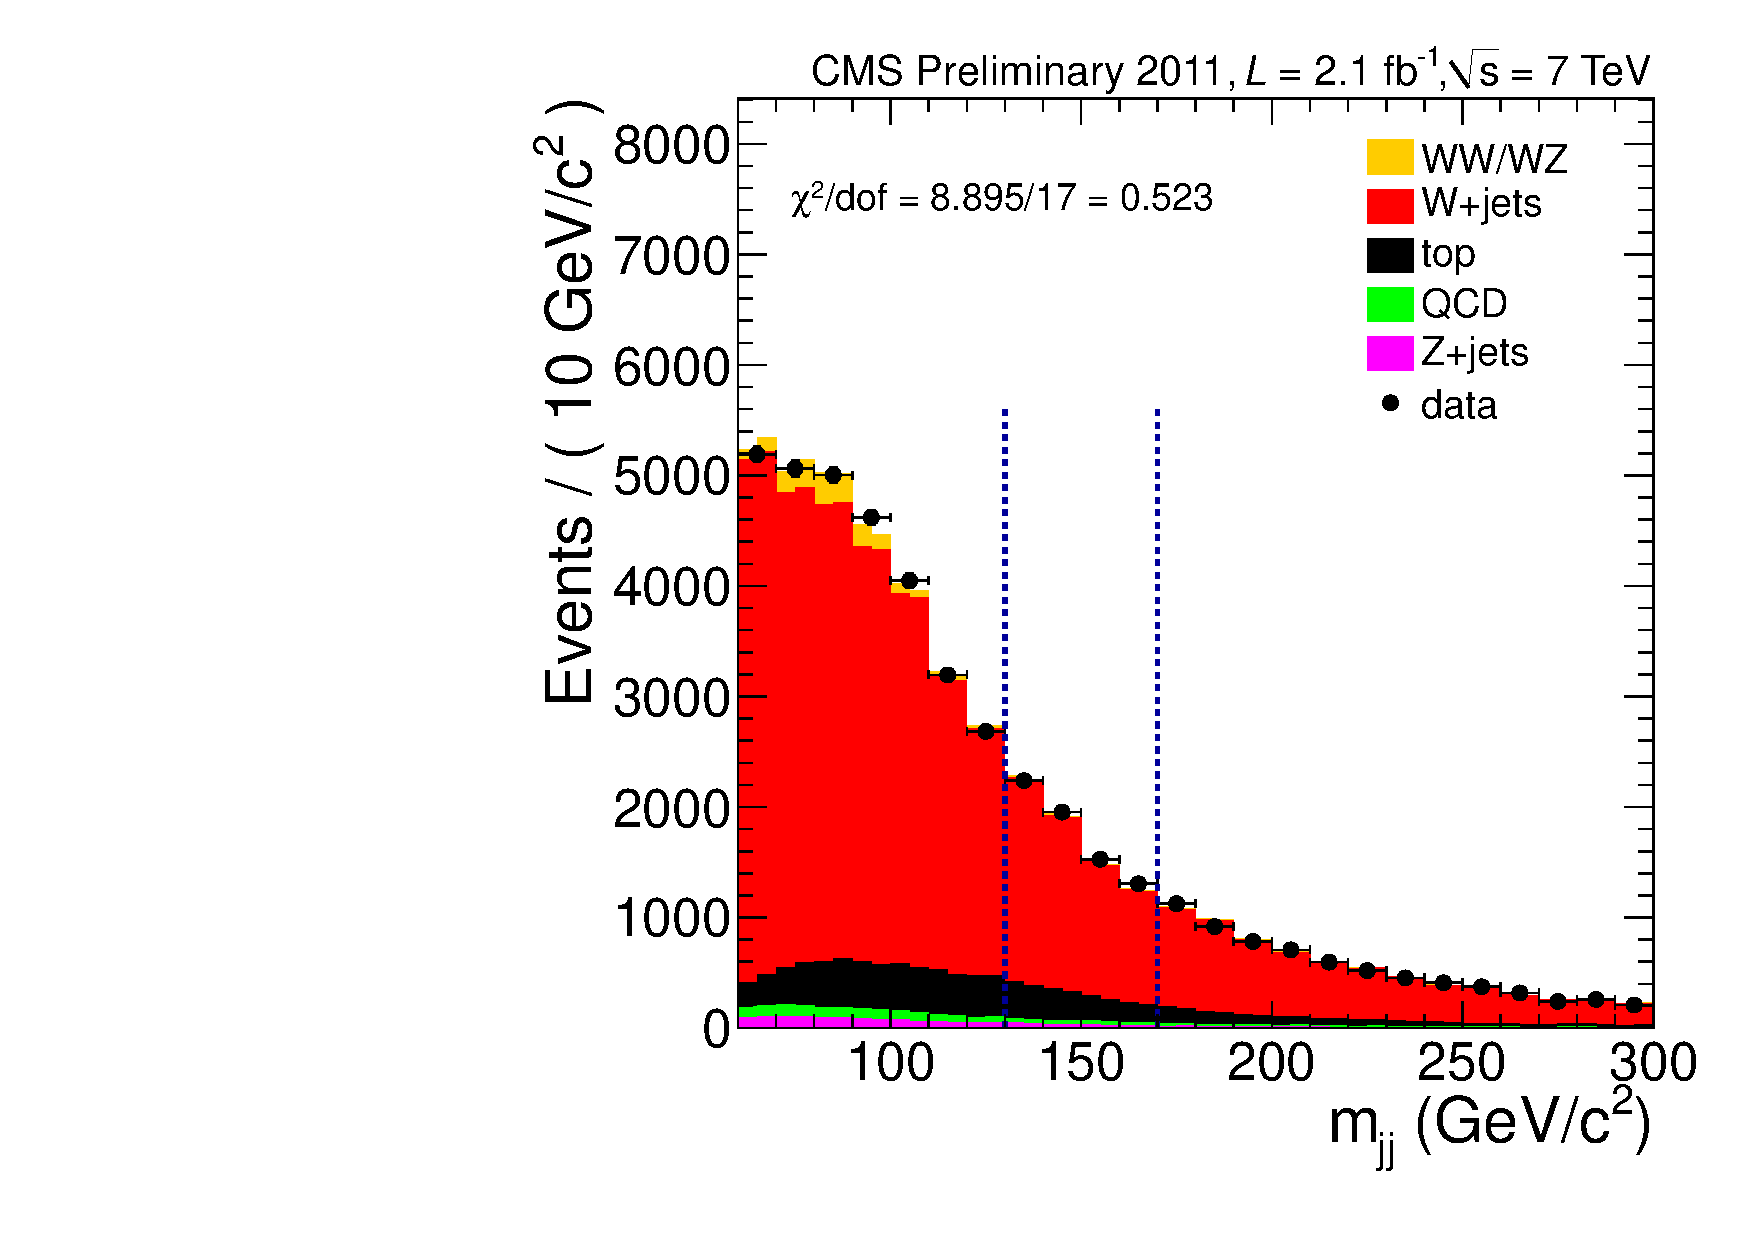
\includegraphics[width=0.49\textwidth]{figs/mjjfit_2jetsample/Wjj_Mjj_2jets_Stacked.pdf}
%    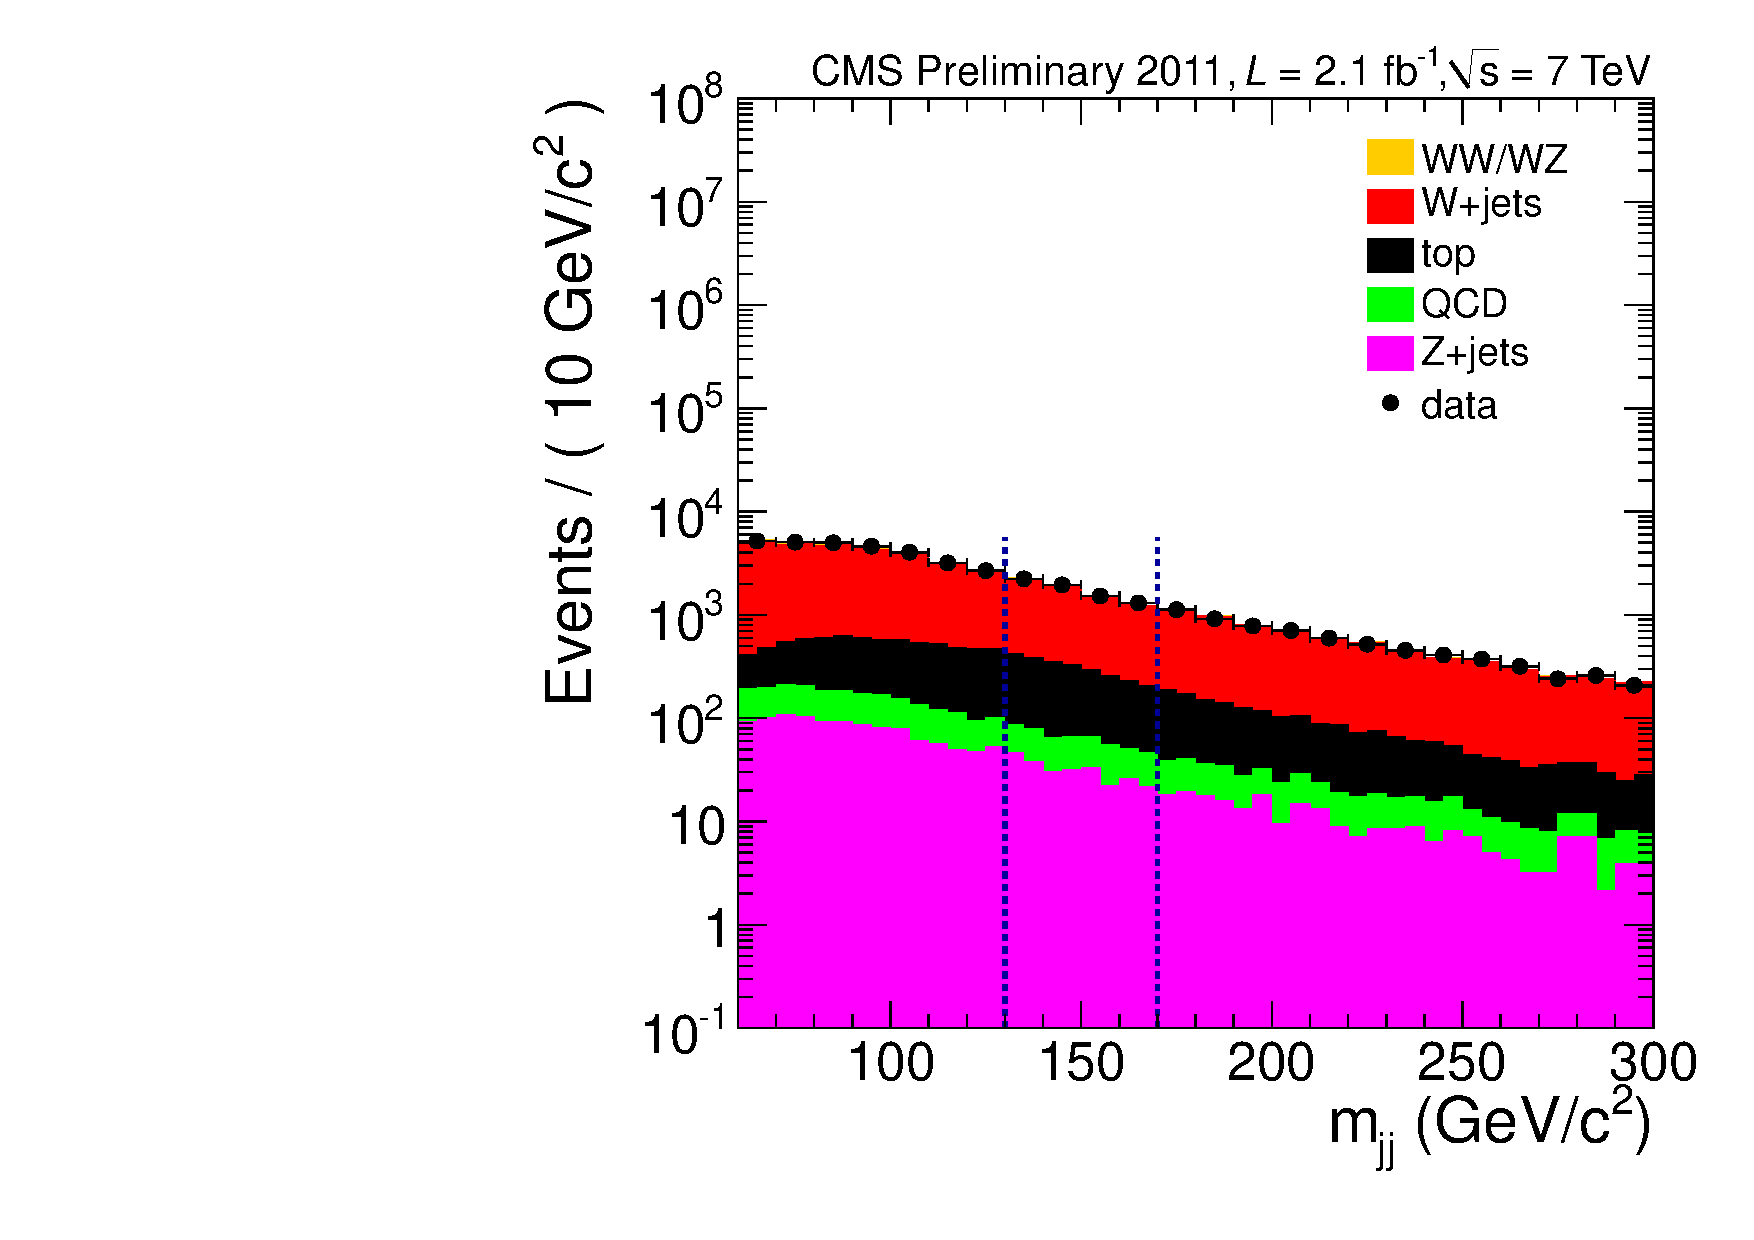
\includegraphics[width=0.49\textwidth]{figs/mjjfit_2jetsample/Wjj_Mjj_2jets_Stacked_log.pdf}
%    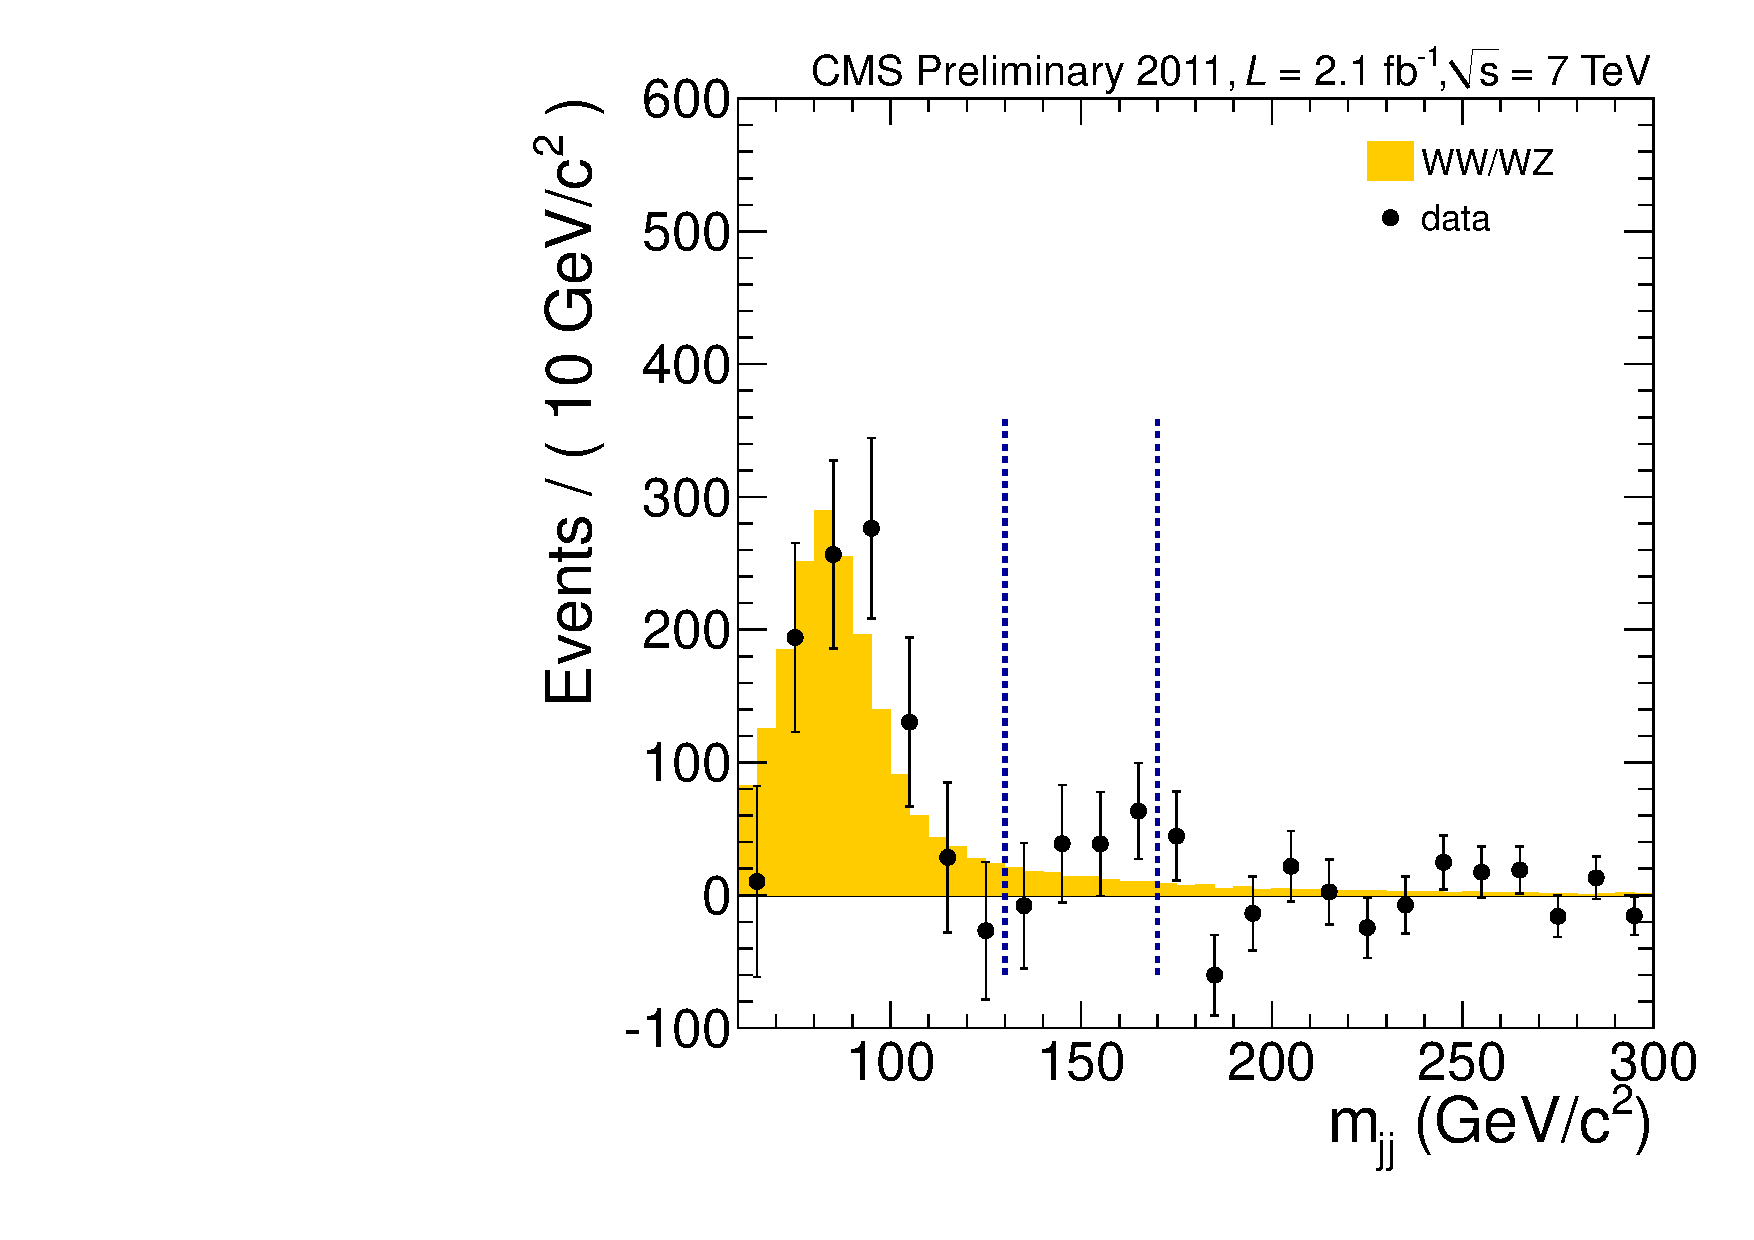
\includegraphics[width=0.49\textwidth]{figs/mjjfit_2jetsample/Wjj_Mjj_2jets_Subtracted.pdf}
%    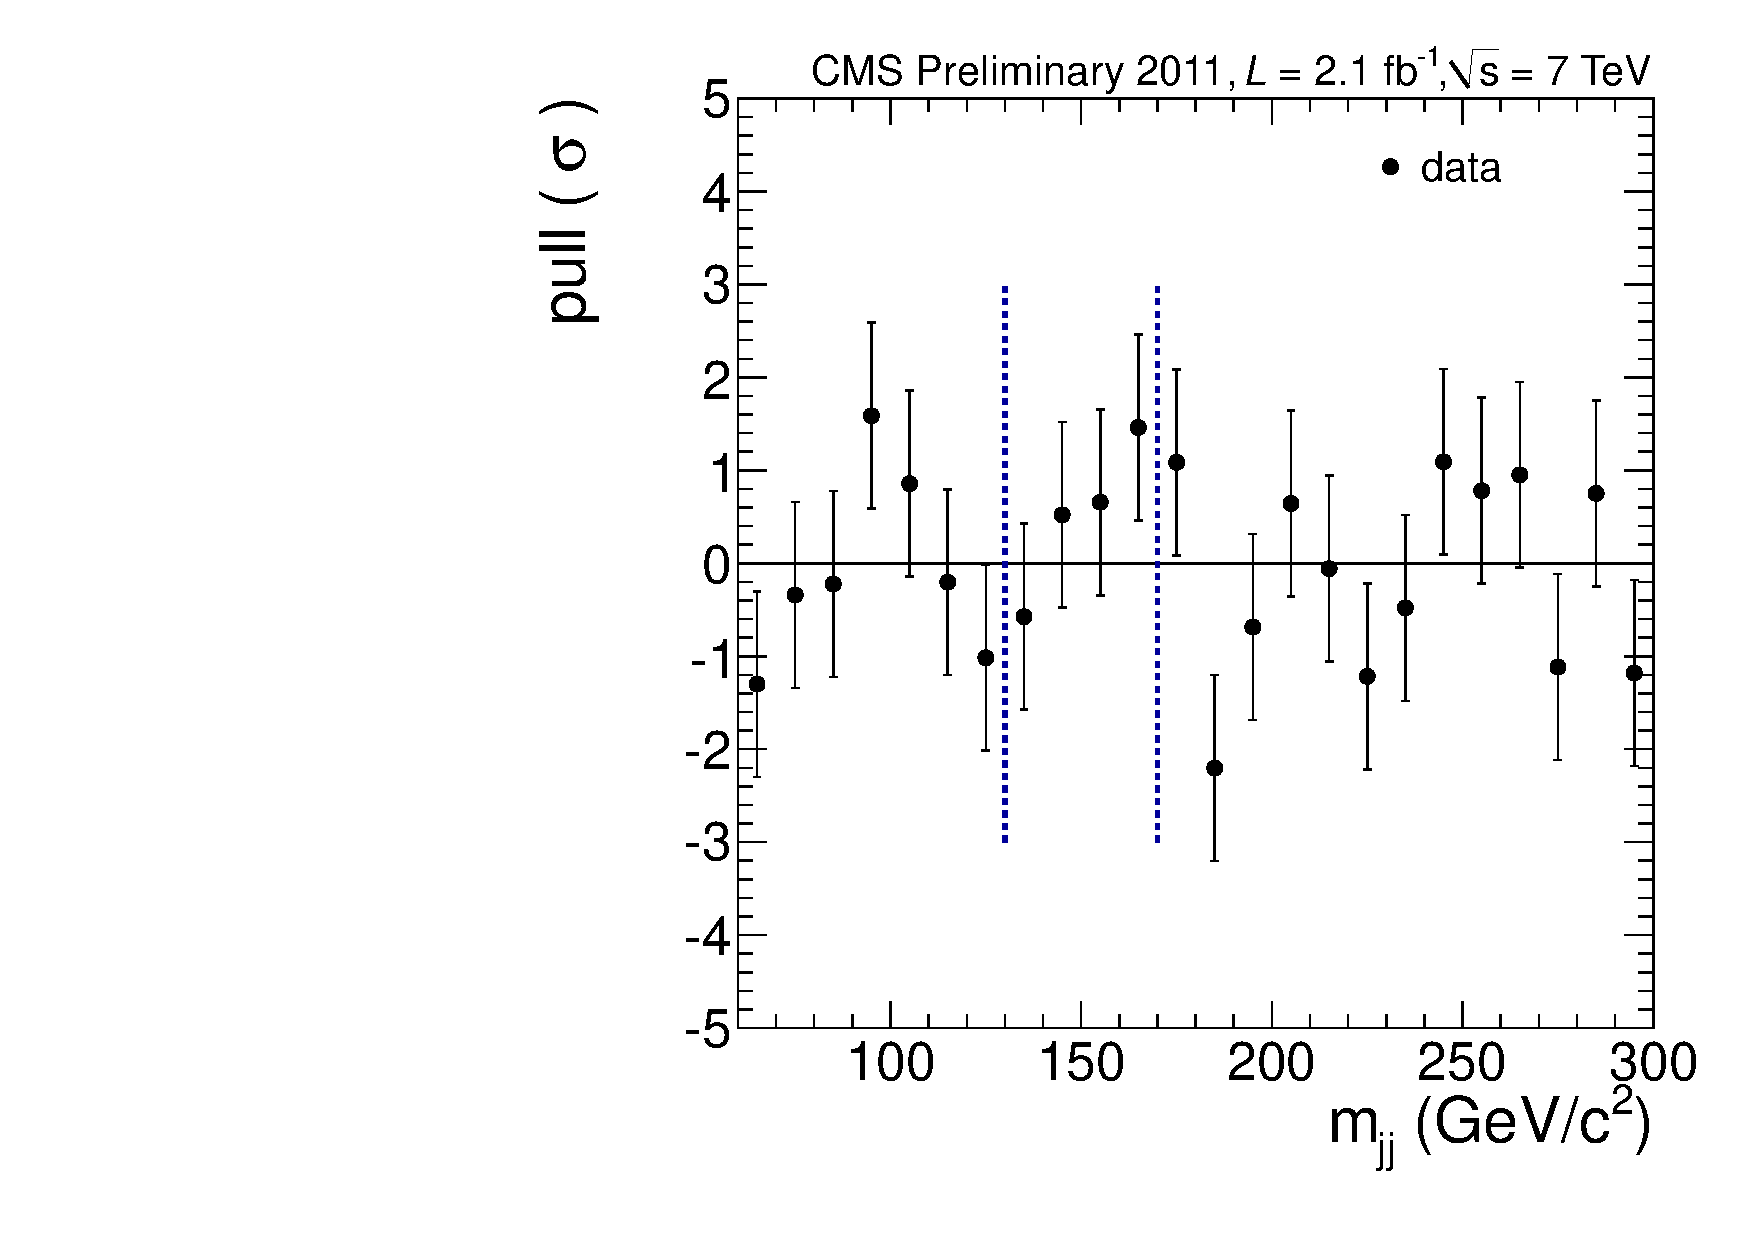
\includegraphics[width=0.49\textwidth]{figs/mjjfit_2jetsample/Wjj_Mjj_2jets_Pull.pdf}

%    \caption{Distribution of the dijet invariant mass for the 2-jet events in data and Monte Carlo: 
%      (upper left) All background components stacked together, 
%      (upper right) unstacked, (lower left) [Data minus all backgrounds except diboson],  
%      (lower right) normalized residual between data and MC. The vertical dotted lines
%      indicate the mass interval excluded from the fit.}
%    \label{fig:mjj_2jet}}
%\end{figure}
%%%%%%%%%%%%%%%%%%%%
%%%%%%%%%%%%%%%%%%%%
\begin{figure}[h!]
  {\centering
    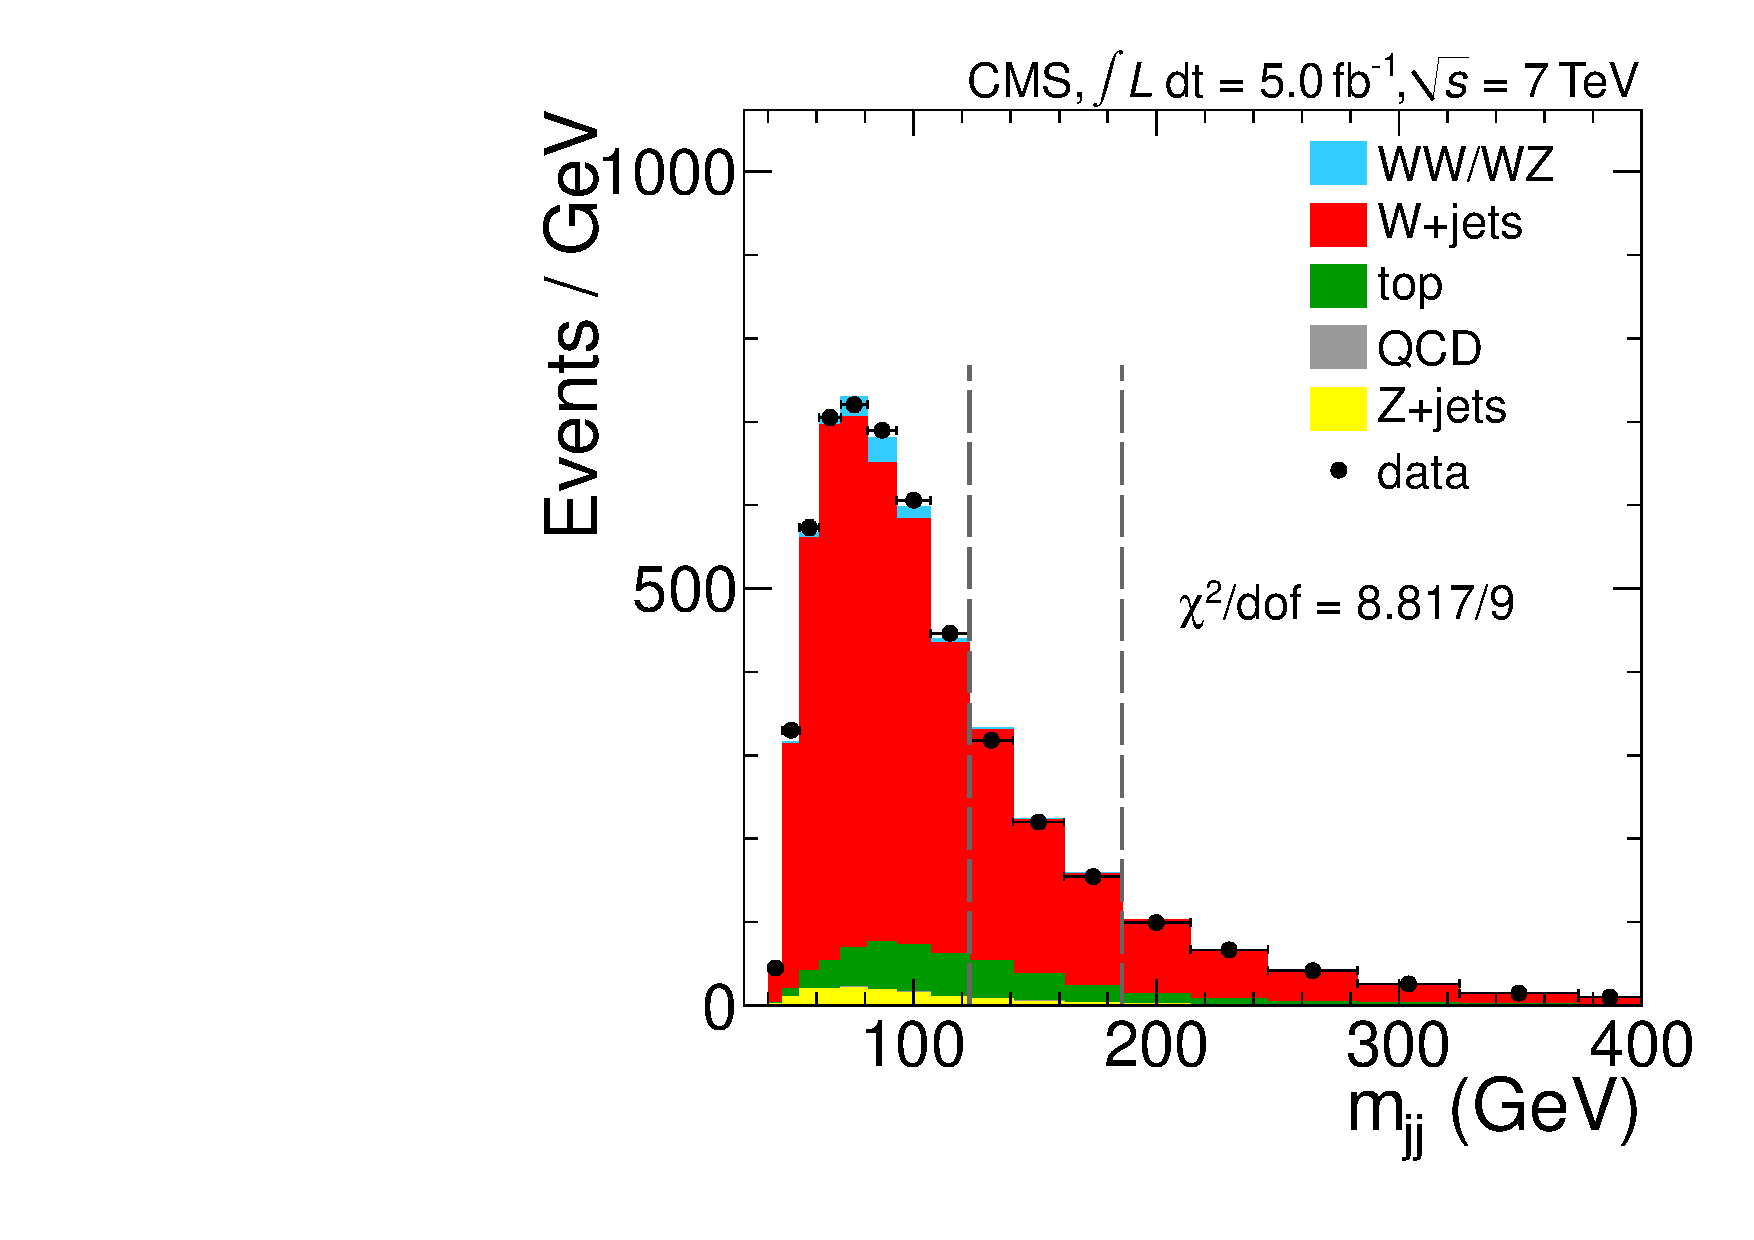
\includegraphics[width=0.49\textwidth]{figs/mjjfit_2jetsample/Wjj_Mjj_Muon_2jets_Stacked.pdf}
    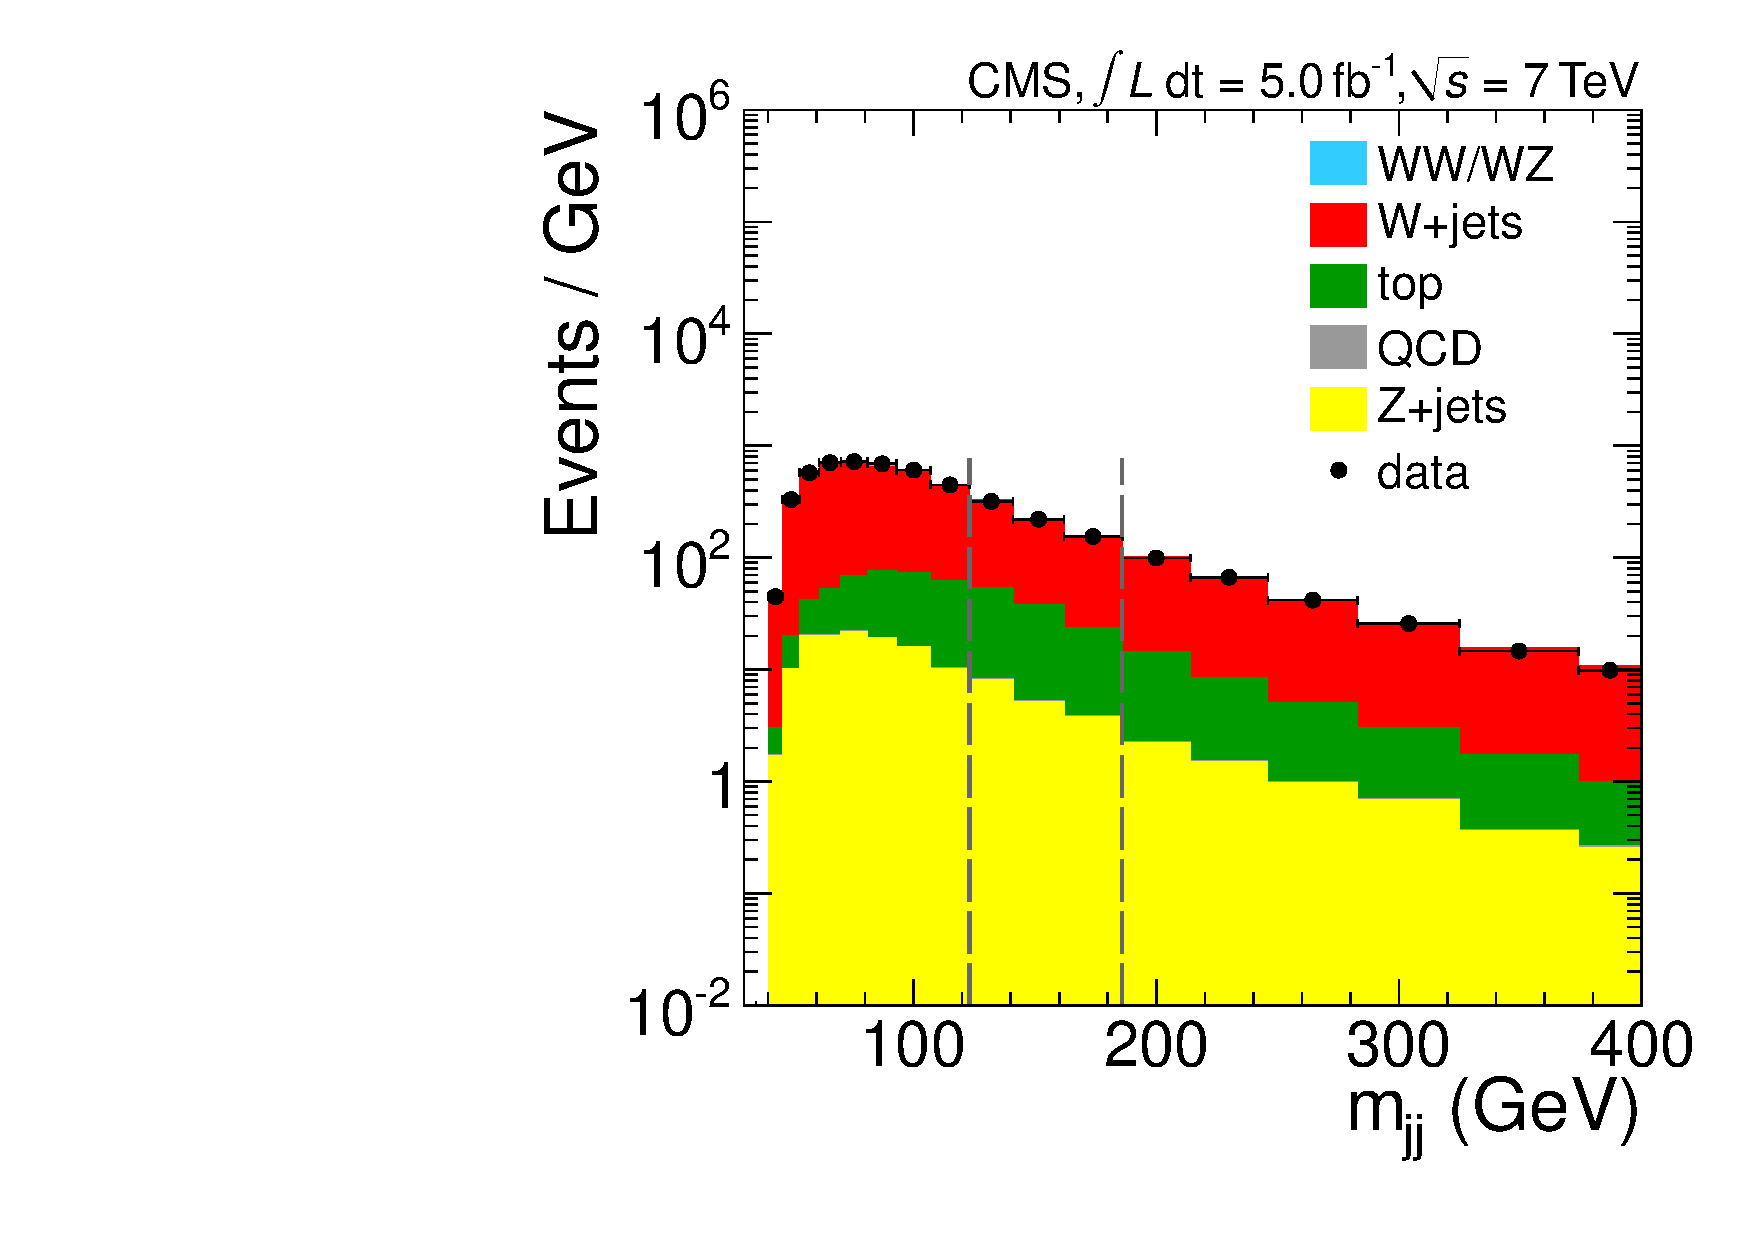
\includegraphics[width=0.49\textwidth]{figs/mjjfit_2jetsample/Wjj_Mjj_Muon_2jets_Stacked_log.pdf}
    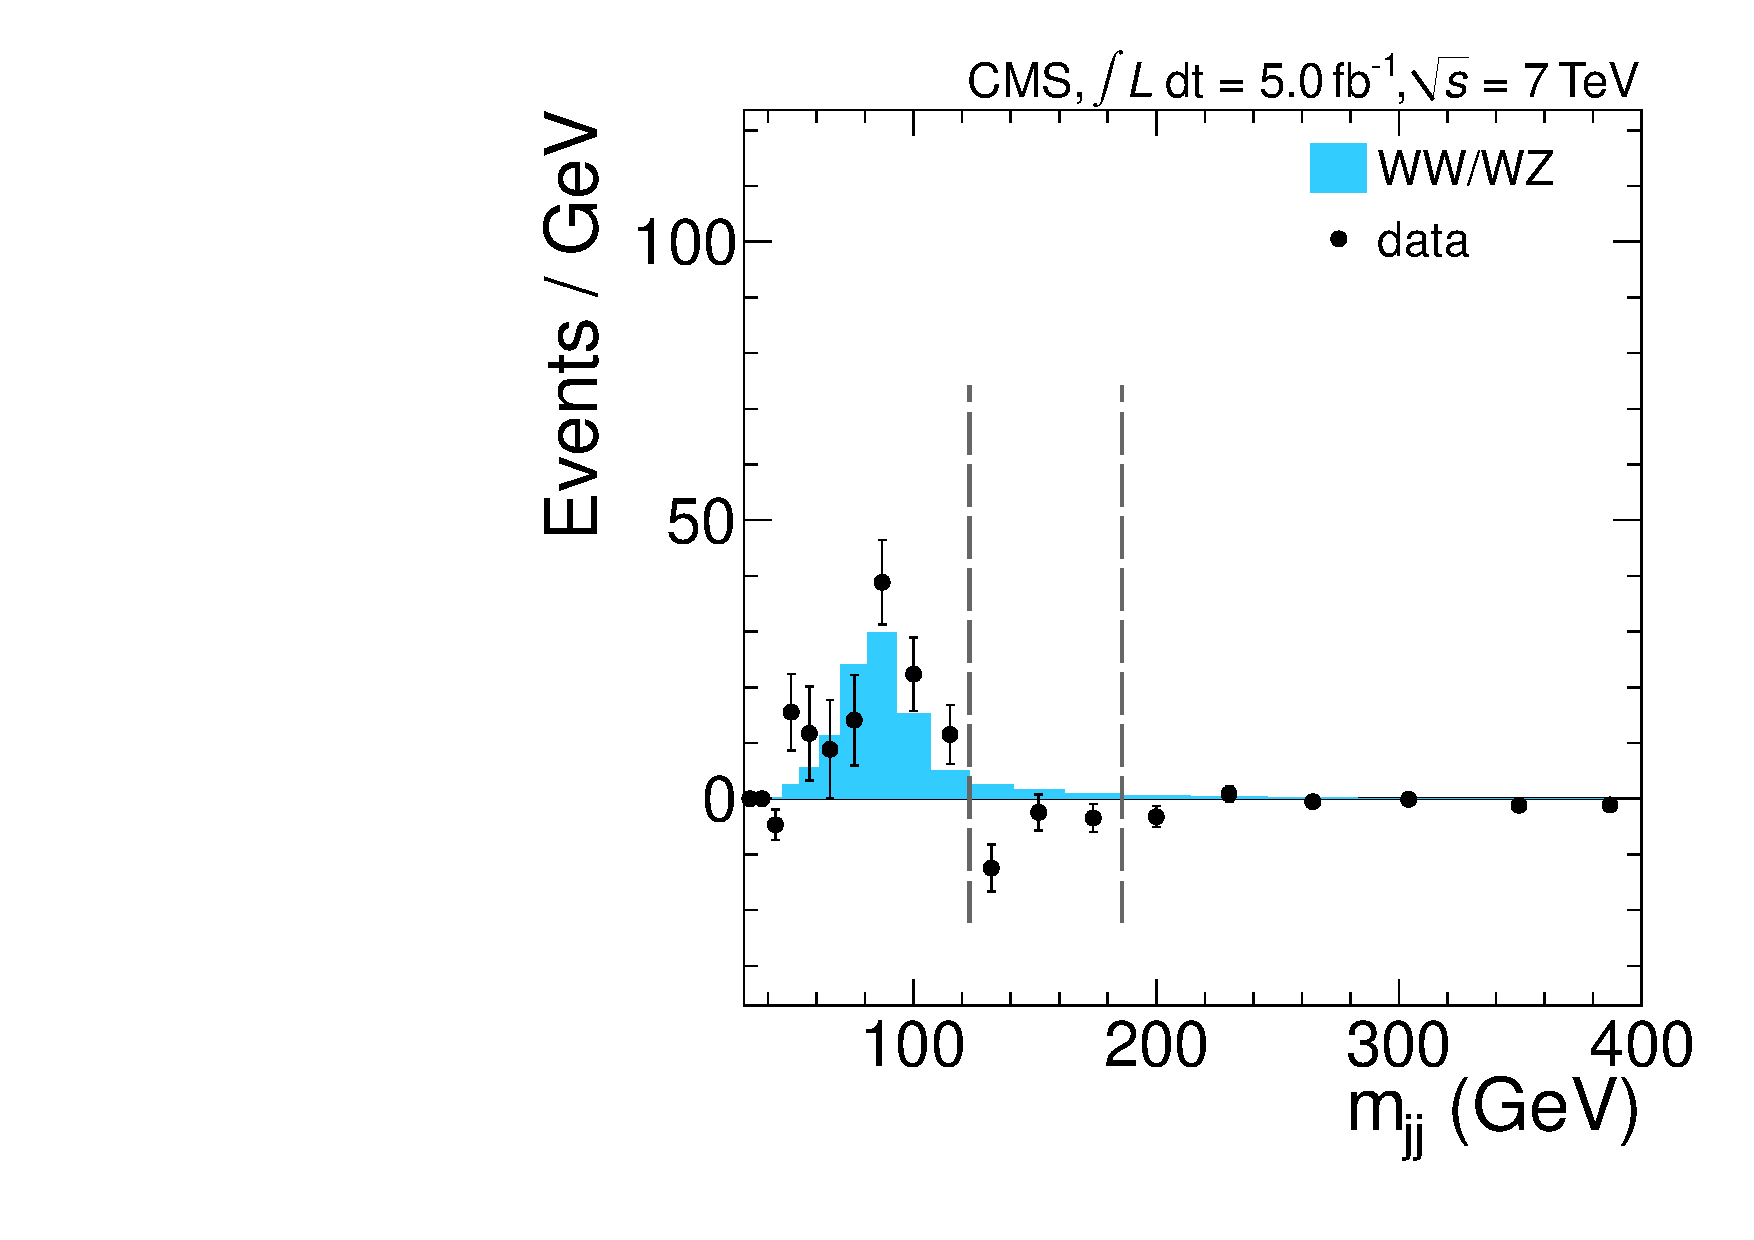
\includegraphics[width=0.49\textwidth]{figs/mjjfit_2jetsample/Wjj_Mjj_Muon_2jets_Subtracted.pdf}
    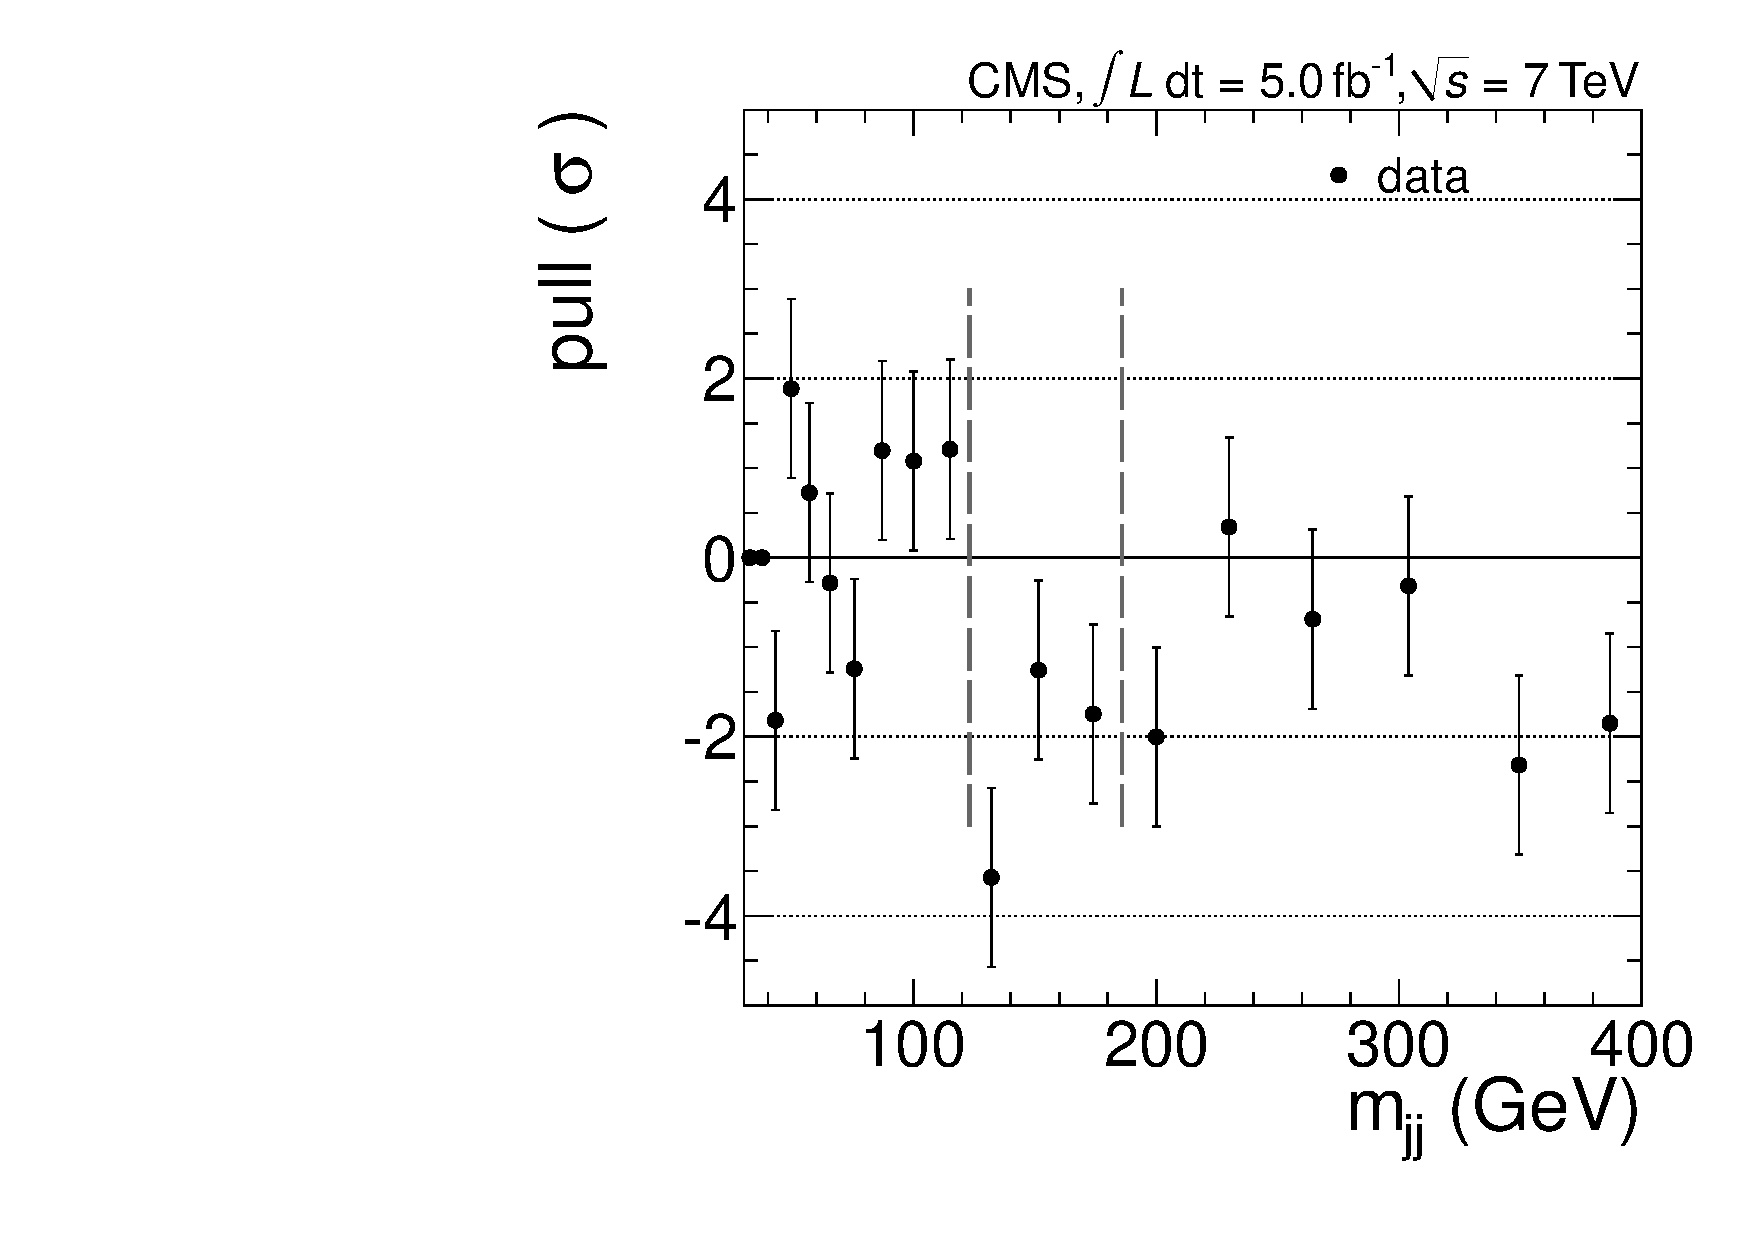
\includegraphics[width=0.49\textwidth]{figs/mjjfit_2jetsample/Wjj_Mjj_Muon_2jets_Pull.pdf}
    \caption{Distribution of the dijet invariant mass for the 2-jet events in muon data and Monte Carlo: 
      (upper left) All background components stacked together, 
      (upper right) unstacked, (lower left) [Data minus all backgrounds except diboson],  
      (lower right) normalized residual between data and MC. The vertical dotted lines
      indicate the mass interval excluded from the fit.}
    \label{fig:mjj_2jet_mu}}
\end{figure}
%%%%%%%%%%%%%%%%%%%%
%%%%%%%%%%%%%%%%%%%%
\begin{figure}[h!]
  {\centering
    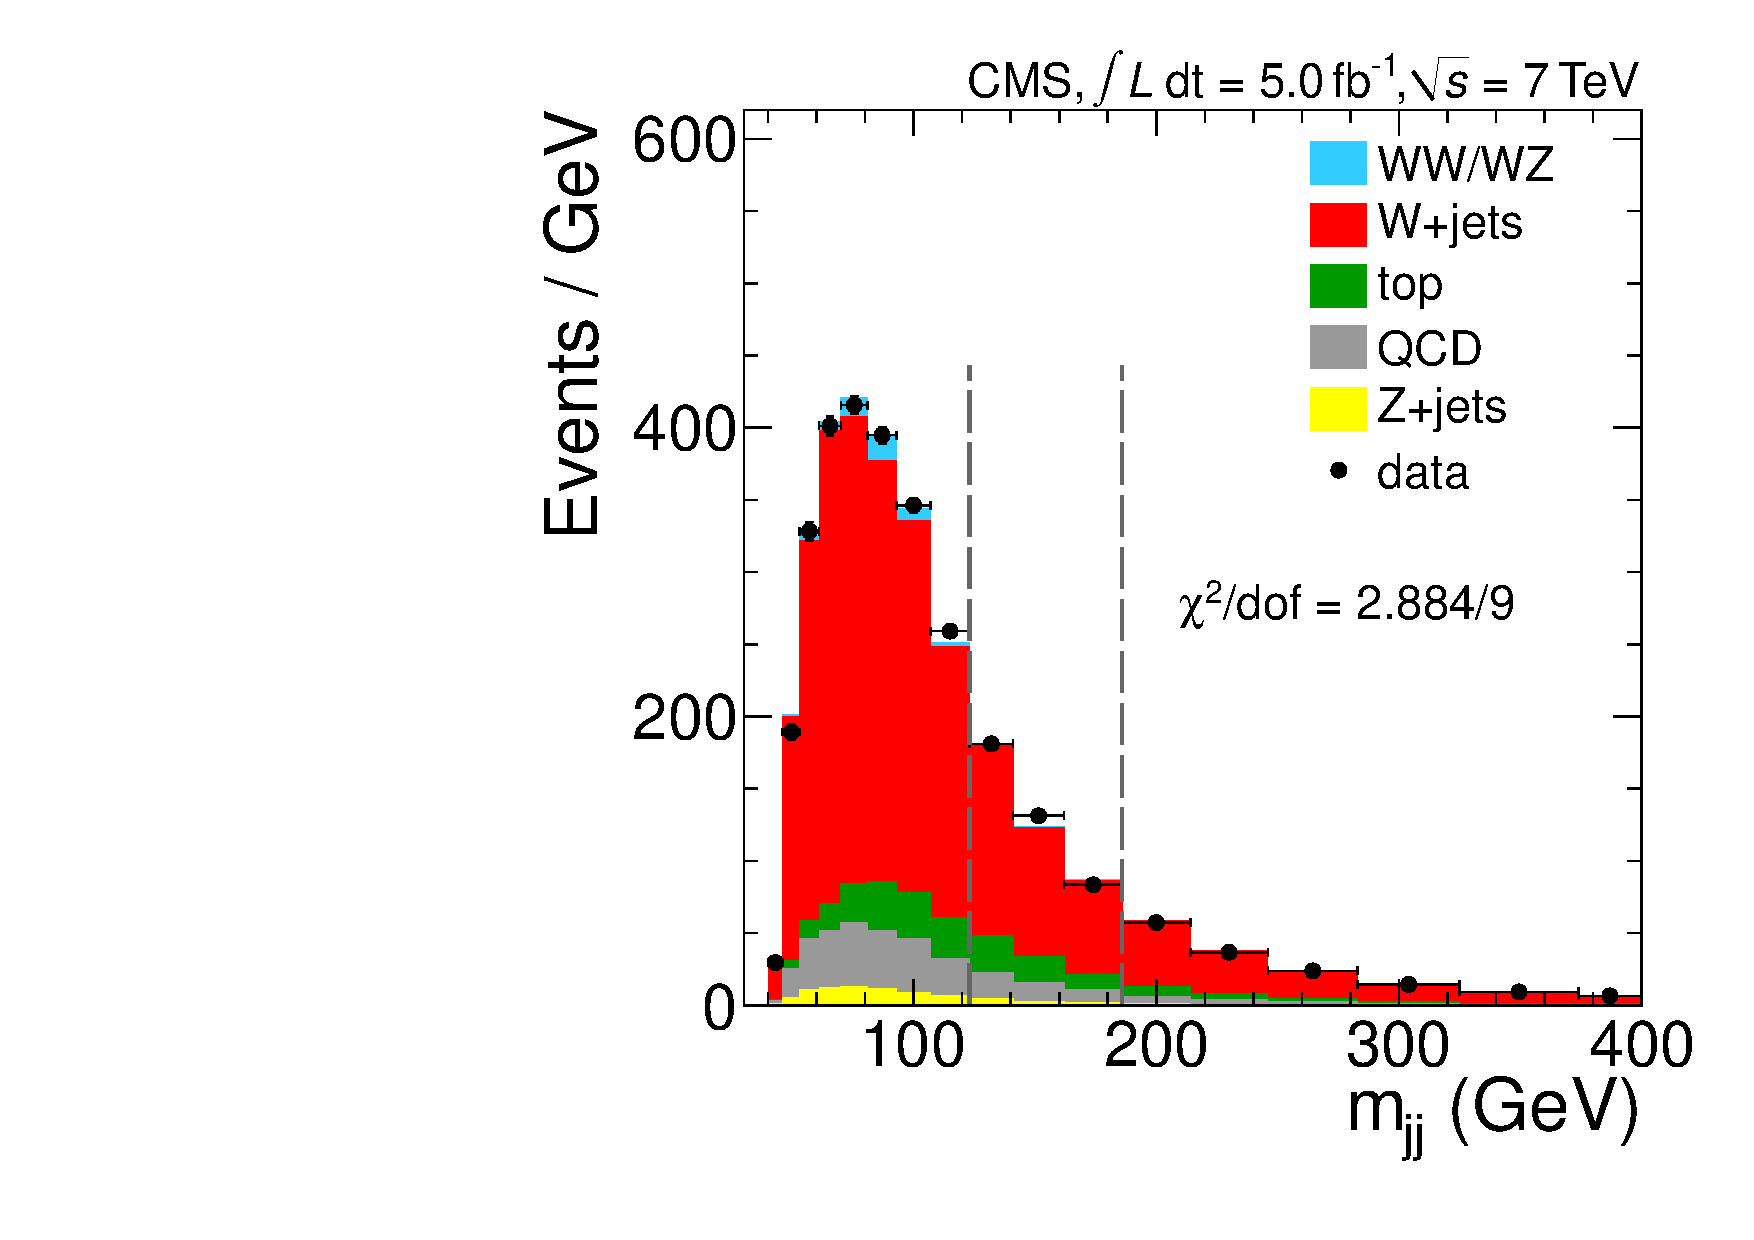
\includegraphics[width=0.49\textwidth]{figs/mjjfit_2jetsample/Wjj_Mjj_Electron_2jets_Stacked.pdf}
    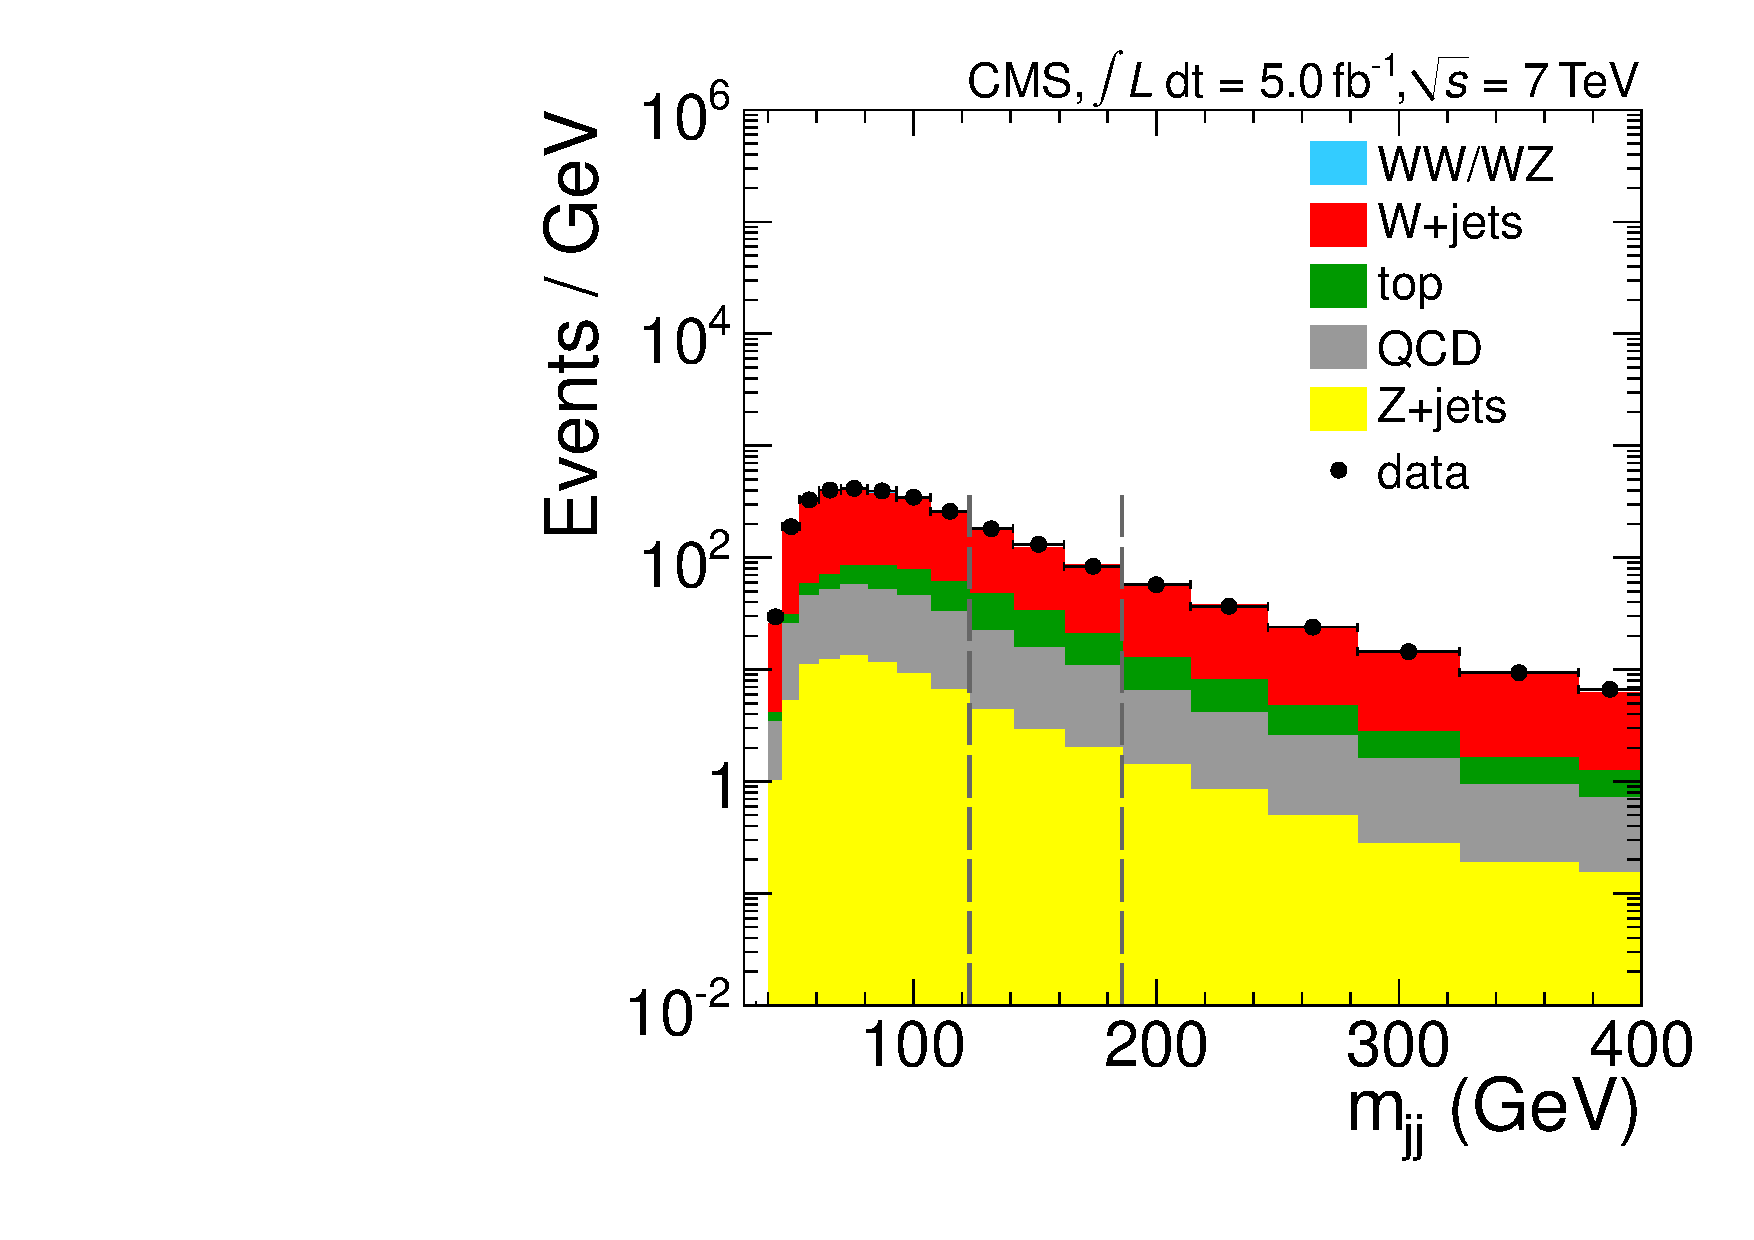
\includegraphics[width=0.49\textwidth]{figs/mjjfit_2jetsample/Wjj_Mjj_Electron_2jets_Stacked_log.pdf}
    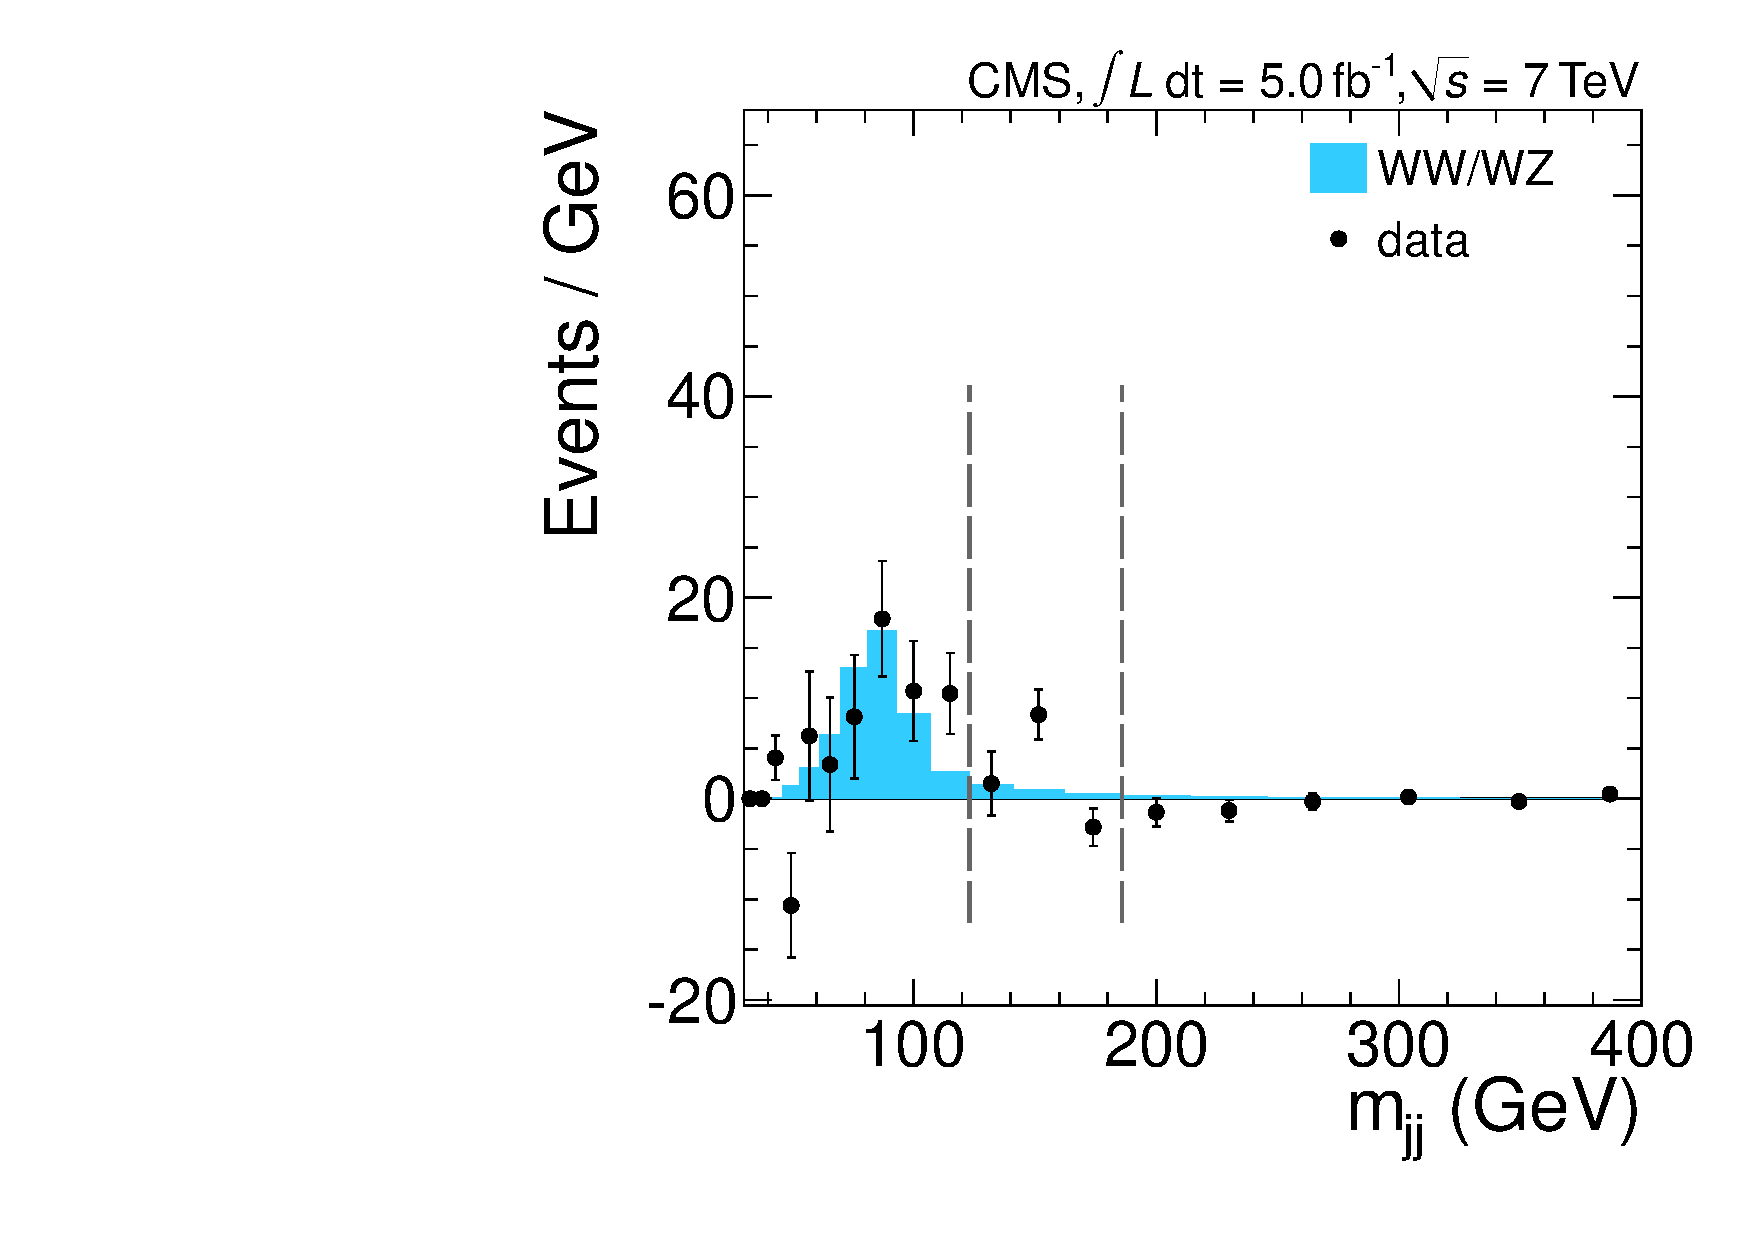
\includegraphics[width=0.49\textwidth]{figs/mjjfit_2jetsample/Wjj_Mjj_Electron_2jets_Subtracted.pdf}
    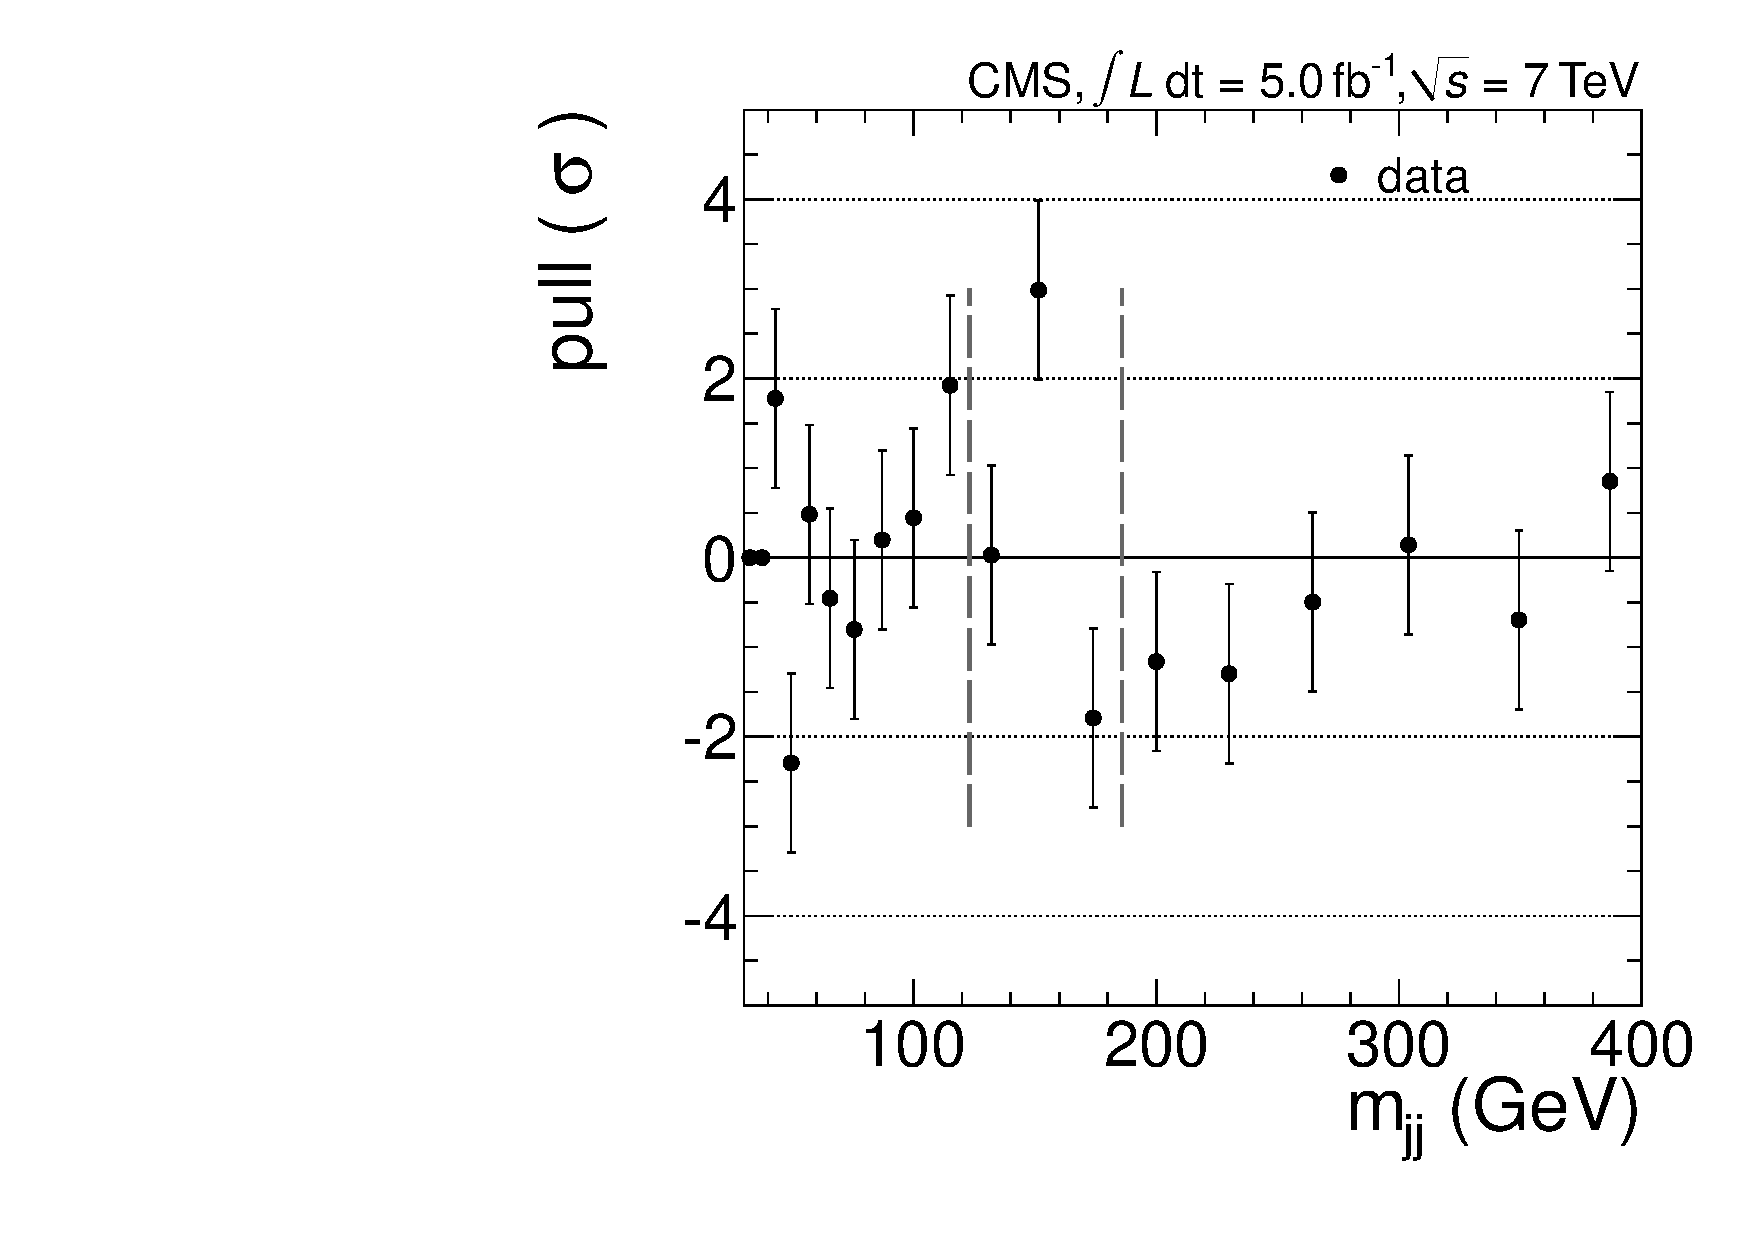
\includegraphics[width=0.49\textwidth]{figs/mjjfit_2jetsample/Wjj_Mjj_Electron_2jets_Pull.pdf}

    \caption{Distribution of the dijet invariant mass for the 2-jet events in electron data and Monte Carlo: 
      (upper left) All background components stacked together, 
      (upper right) unstacked, (lower left) [Data minus all backgrounds except diboson],  
      (lower right) normalized residual between data and MC. The vertical dotted lines
      indicate the mass interval excluded from the fit.}
    \label{fig:mjj_2jet_el}}
\end{figure}
%%%%%%%%%%%%%%%%%%%%
%%%%%%%%%%%%%%%%%%%%
\clearpage
%%%%%%%%%%%%%%%%%%%%%%%%%%%%%%%%%%%%%%%%%%%%%%%%%%%%%%%%%%%%
%%%%%%%%%%%%%%%%%%%%%%%%%%%%%%%%%%%%%%%%%%%%%%%%%%%%%%%%%%%%
\subsection{Fit results for the 3-jet sample}
\label{sec:mjj_3jetfit}
The results of the fit for the 3-jet sample are shown 
in Figs.~\ref{fig:mjj_3jet_mu} and~\ref{fig:mjj_3jet_el}. 
The peak from the Standard Model electroweak diboson 
WW/WZ production is significantly smaller than the one in 2-jet sample. 
The diboson and other yields are 
consistent with the Standard Model NLO predictions.
The fit results are tabulated below.
%%%%%%%%%%%%%%%%%%%%

Muons
{\footnotesize
\begin{verbatim}
 COVARIANCE MATRIX CALCULATED SUCCESSFULLY
 FCN=-55938.6 FROM HESSE     STATUS=OK             54 CALLS         282 TOTAL
                     EDM=0.00126466    STRATEGY= 1      ERROR MATRIX ACCURATE 
  EXT PARAMETER                                INTERNAL      INTERNAL  
  NO.   NAME      VALUE            ERROR       STEP SIZE       VALUE   
   1  fMU         -3.01854e-05   9.29560e-03   1.17892e-03  -3.01854e-05
   2  fSU          1.62702e-01   1.01444e-01   6.63014e-03   1.63428e-01
   3  nDiboson     3.32924e+02   3.25068e+01   5.20139e+00   3.32924e+02
   4  nSingleTop   1.00112e+03   4.97330e+01   7.84979e+00   1.00112e+03
   5  nTTbar       9.04906e+03   3.81876e+02   3.06769e+01   9.04906e+03
   6  nWjets       1.30694e+04   3.66179e+02   2.90971e+01   1.30694e+04
   7  nZjets       5.60638e+02   2.40755e+01   3.89477e+00   5.60638e+02
                               ERR DEF= 0.5
 EXTERNAL ERROR MATRIX.    NDIM=  25    NPAR=  7    ERR DEF=0.5
  8.641e-05  7.721e-07  4.426e-04  5.730e-04  2.532e-02 -3.033e-02  2.515e-05 
  7.721e-07  1.033e-02  1.444e-01  9.548e-02  2.925e-01  2.510e+00  1.042e-02 
  4.426e-04  1.444e-01  1.057e+03 -5.045e+00 -3.697e+01 -1.079e+03 -4.624e-01 
  5.730e-04  9.548e-02 -5.045e+00  2.473e+03 -9.285e+02 -1.508e+03 -6.620e-01 
  2.532e-02  2.925e-01 -3.697e+01 -9.285e+02  1.458e+05 -1.193e+05 -6.452e+01 
 -3.033e-02  2.510e+00 -1.079e+03 -1.508e+03 -1.193e+05  1.341e+05 -5.364e+02 
  2.515e-05  1.042e-02 -4.624e-01 -6.620e-01 -6.452e+01 -5.364e+02  5.796e+02 
 PARAMETER  CORRELATION COEFFICIENTS  
       NO.  GLOBAL      1      2      3      4      5      6      7
        1  0.00912   1.000  0.001  0.001  0.001  0.007 -0.009  0.000
        2  0.17050   0.001  1.000  0.044  0.019  0.008  0.067  0.004
        3  0.20022   0.001  0.044  1.000 -0.003 -0.003 -0.091 -0.001
        4  0.25668   0.001  0.019 -0.003  1.000 -0.049 -0.083 -0.001
        5  0.87038   0.007  0.008 -0.003 -0.049  1.000 -0.853 -0.007
        6  0.87341  -0.009  0.067 -0.091 -0.083 -0.853  1.000 -0.061
        7  0.13725   0.000  0.004 -0.001 -0.001 -0.007 -0.061  1.000

  RooFitResult: minimized FCN value: -55938.6, estimated distance to minimum: 0.00126466
                covariance matrix quality: Full, accurate covariance matrix

    Constant Parameter    Value     
  --------------------  ------------
                  nQCD    0.0000e+00

    Floating Parameter  InitialValue    FinalValue +/-  Error     GblCorr.
  --------------------  ------------  --------------------------  --------
                   fMU   -1.0000e-01   -3.0185e-05 +/-  9.30e-03  <none>
                   fSU    3.0000e-01    1.6270e-01 +/-  1.01e-01  <none>
              nDiboson    3.2000e+02    3.3292e+02 +/-  3.25e+01  <none>
            nSingleTop    8.5800e+02    1.0011e+03 +/-  4.97e+01  <none>
                nTTbar    6.5000e+03    9.0491e+03 +/-  3.82e+02  <none>
                nWjets    1.3000e+04    1.3069e+04 +/-  3.66e+02  <none>
                nZjets    4.0000e+02    5.6064e+02 +/-  2.41e+01  <none>

total yield: 24013 +/- 193
\end{verbatim}
}

Electrons
{\footnotesize
\begin{verbatim}
 COVARIANCE MATRIX CALCULATED SUCCESSFULLY
 FCN=-28298.2 FROM HESSE     STATUS=OK             61 CALLS         280 TOTAL
                     EDM=3.35978e-05    STRATEGY= 1      ERROR MATRIX ACCURATE 
  EXT PARAMETER                                INTERNAL      INTERNAL  
  NO.   NAME      VALUE            ERROR       STEP SIZE       VALUE   
   1  fMU          2.50071e-01   1.11216e-01   5.24358e-04   2.52753e-01
   2  fSU          2.95883e-02   6.37407e-02   1.46508e-03   2.95926e-02
   3  nDiboson     1.84223e+02   1.83482e+01   4.21697e-01   1.84223e+02
   4  nQCD         3.23934e+02   1.60155e+02   2.44661e+00   3.23934e+02
   5  nSingleTop   5.21195e+02   2.61655e+01   5.98480e-01   5.21195e+02
   6  nTTbar       4.26483e+03   2.52878e+02   3.18636e+00   4.26483e+03
   7  nWjets       8.39696e+03   2.92476e+02   3.15929e+00   8.39696e+03
   8  nZjets       3.63923e+02   1.56398e+01   3.60887e-01   3.63923e+02
                               ERR DEF= 0.5
 EXTERNAL ERROR MATRIX.    NDIM=  25    NPAR=  8    ERR DEF=0.5
  1.242e-02 -7.384e-04  5.725e-02  1.415e-01  1.895e-02 -4.548e+00  4.164e+00  7.189e-03 
 -7.384e-04  4.068e-03  1.132e-02 -6.575e-01  1.273e-02  1.082e+00 -9.971e-01 -3.284e-03 
  5.725e-02  1.132e-02  3.367e+02 -2.057e+01 -1.068e+00 -2.833e+01 -3.154e+02  2.715e-02 
  1.415e-01 -6.575e-01 -2.057e+01  2.565e+04 -2.744e+01 -1.417e+03 -2.357e+04 -1.613e+00 
  1.895e-02  1.273e-02 -1.068e+00 -2.744e+01  6.846e+02 -1.616e+02 -4.658e+02 -1.714e-02 
 -4.548e+00  1.082e+00 -2.833e+01 -1.417e+03 -1.616e+02  6.395e+04 -5.172e+04  9.915e-01 
  4.164e+00 -9.971e-01 -3.154e+02 -2.357e+04 -4.658e+02 -5.172e+04  8.554e+04 -2.473e+02 
  7.189e-03 -3.284e-03  2.715e-02 -1.613e+00 -1.714e-02  9.915e-01 -2.473e+02  2.446e+02 
 PARAMETER  CORRELATION COEFFICIENTS  
       NO.  GLOBAL      1      2      3      4      5      6      7      8
        1  0.19120   1.000 -0.104  0.028  0.008  0.006 -0.161  0.128  0.004
        2  0.15335  -0.104  1.000  0.010 -0.064  0.008  0.067 -0.053 -0.003
        3  0.14610   0.028  0.010  1.000 -0.007 -0.002 -0.006 -0.059  0.000
        4  0.75324   0.008 -0.064 -0.007  1.000 -0.007 -0.035 -0.503 -0.001
        5  0.17518   0.006  0.008 -0.002 -0.007  1.000 -0.024 -0.061 -0.000
        6  0.83993  -0.161  0.067 -0.006 -0.035 -0.024  1.000 -0.699  0.000
        7  0.88519   0.128 -0.053 -0.059 -0.503 -0.061 -0.699  1.000 -0.054
        8  0.11628   0.004 -0.003  0.000 -0.001 -0.000  0.000 -0.054  1.000

  RooFitResult: minimized FCN value: -28298.2, estimated distance to minimum: 3.35978e-05
                covariance matrix quality: Full, accurate covariance matrix

    Floating Parameter  InitialValue    FinalValue +/-  Error     GblCorr.
  --------------------  ------------  --------------------------  --------
                   fMU    1.0000e-01    2.5007e-01 +/-  1.11e-01  <none>
                   fSU    3.0000e-01    2.9588e-02 +/-  6.37e-02  <none>
              nDiboson    2.3000e+02    1.8422e+02 +/-  1.83e+01  <none>
                  nQCD    3.2500e+02    3.2393e+02 +/-  1.60e+02  <none>
            nSingleTop    5.8000e+02    5.2120e+02 +/-  2.62e+01  <none>
                nTTbar    4.4000e+03    4.2648e+03 +/-  2.53e+02  <none>
                nWjets    9.5000e+03    8.3970e+03 +/-  2.92e+02  <none>
                nZjets    3.9000e+02    3.6392e+02 +/-  1.56e+01  <none>

total yield: 14055 +/- 143
\end{verbatim}
}

%%%%%%%%%%%%%%%%%%%%
%%%%%%%%%%%%%%%%%%%%
\begin{figure}[h!]
  {\centering
    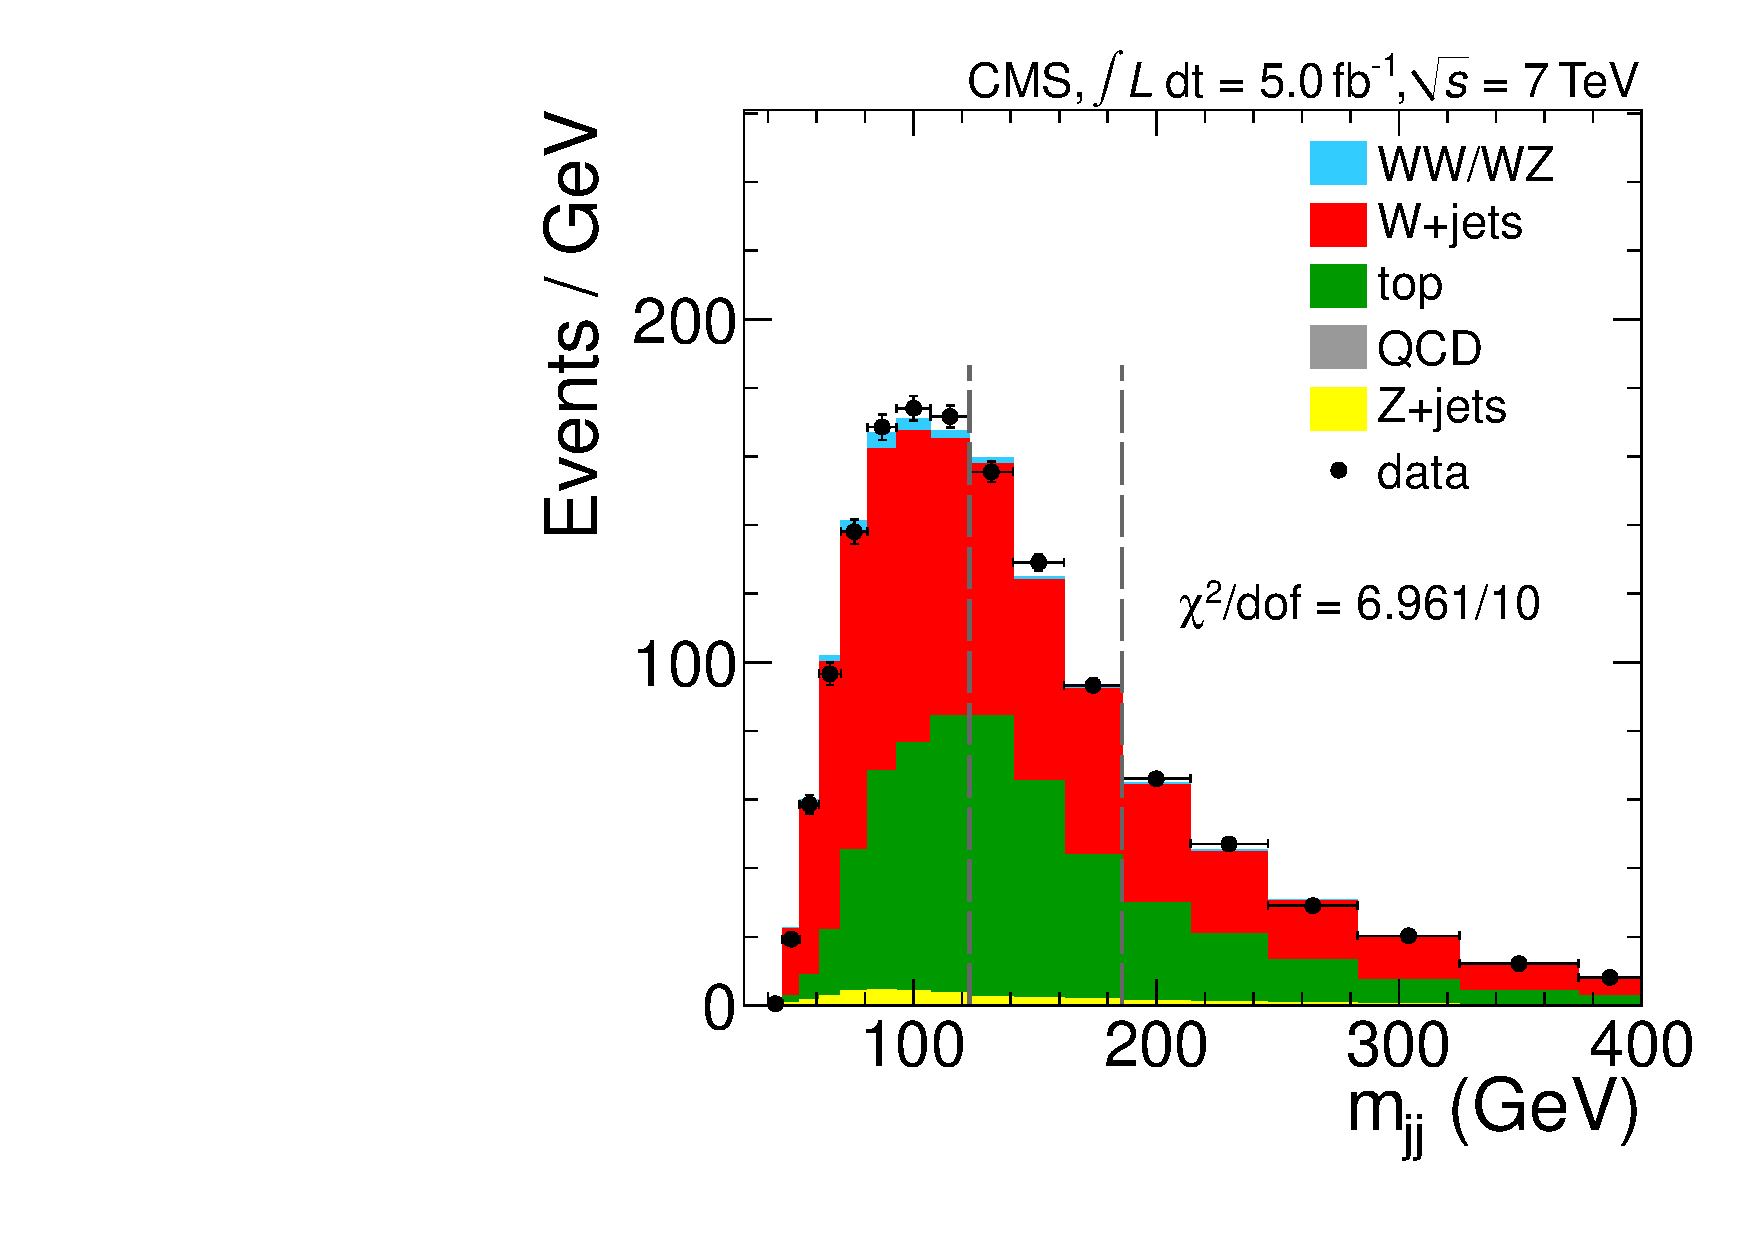
\includegraphics[width=0.49\textwidth]{figs/mjjfit_3jetsample/Wjj_Mjj_Muon_3jets_Stacked.pdf}
    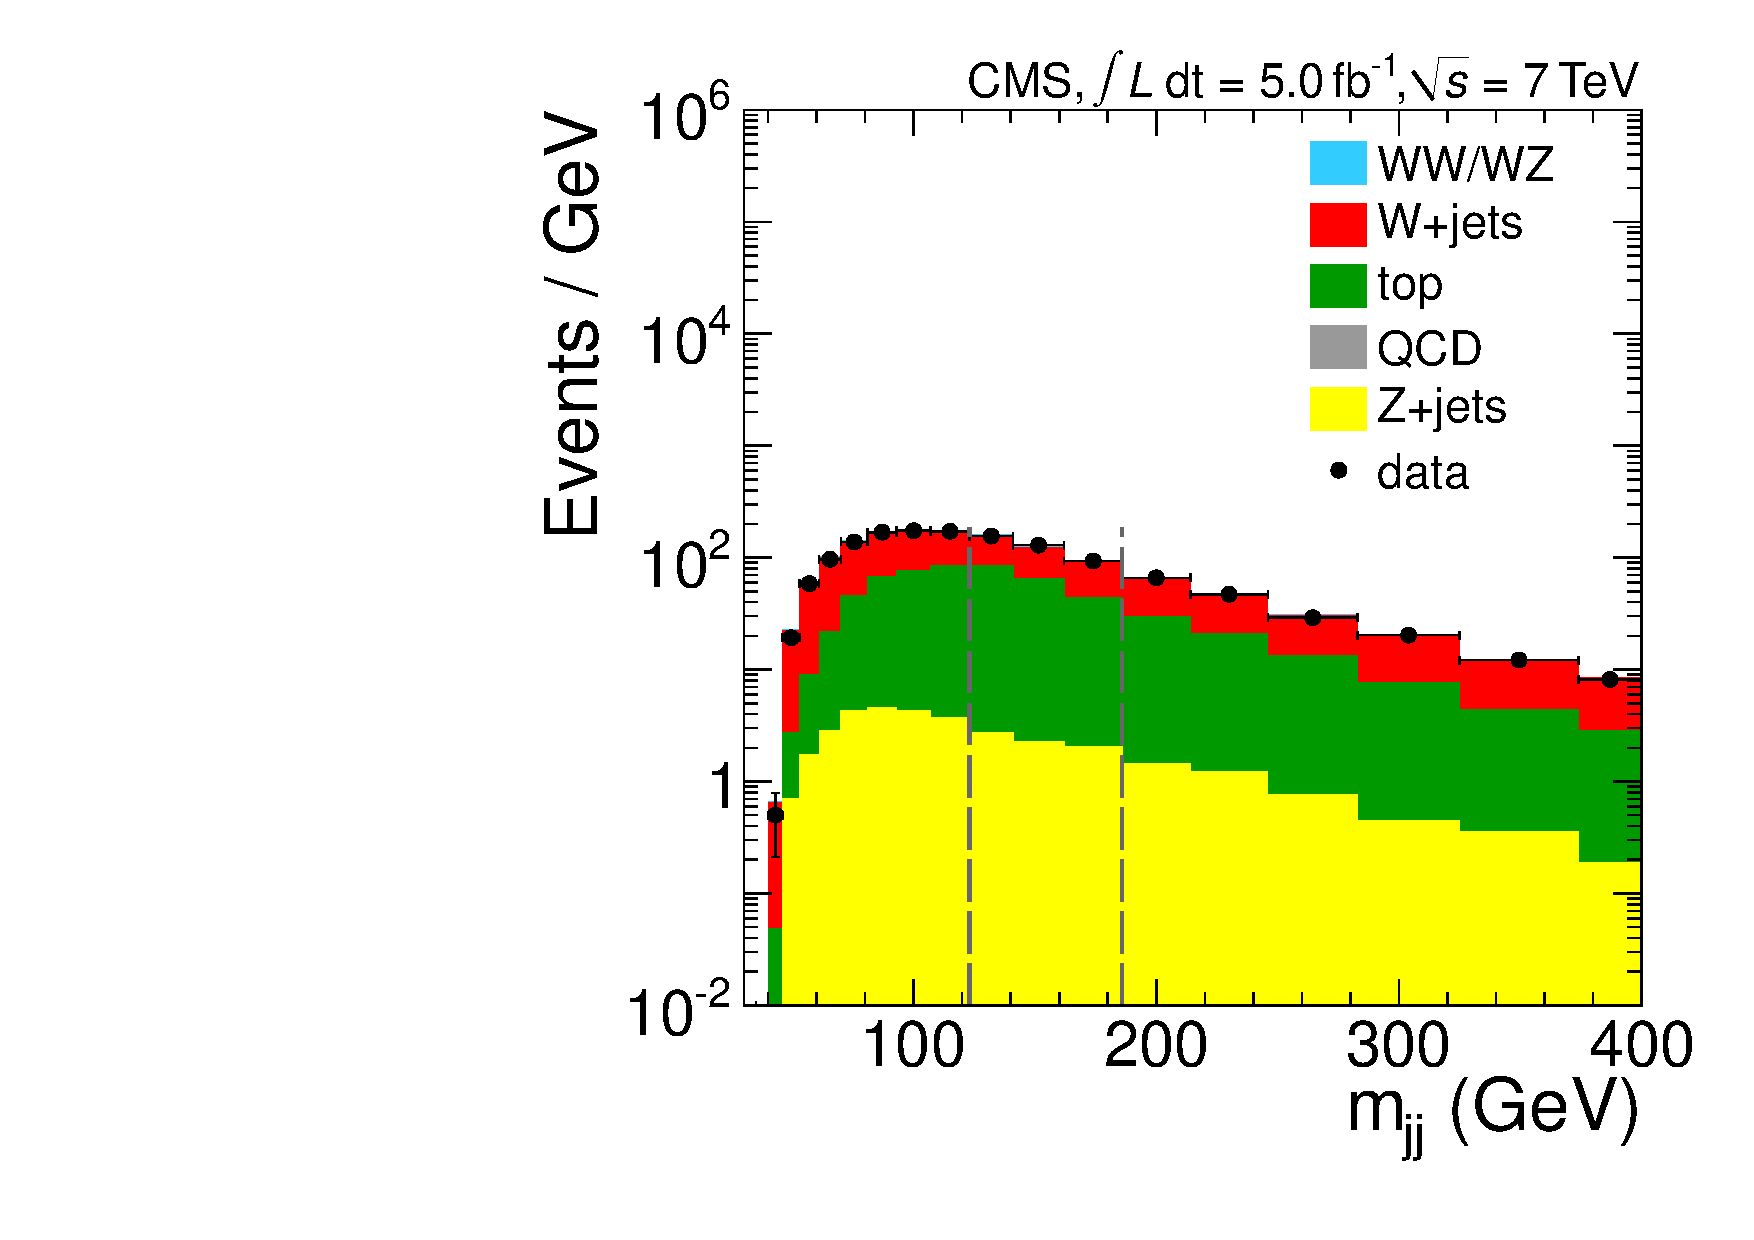
\includegraphics[width=0.49\textwidth]{figs/mjjfit_3jetsample/Wjj_Mjj_Muon_3jets_Stacked_log.pdf}
    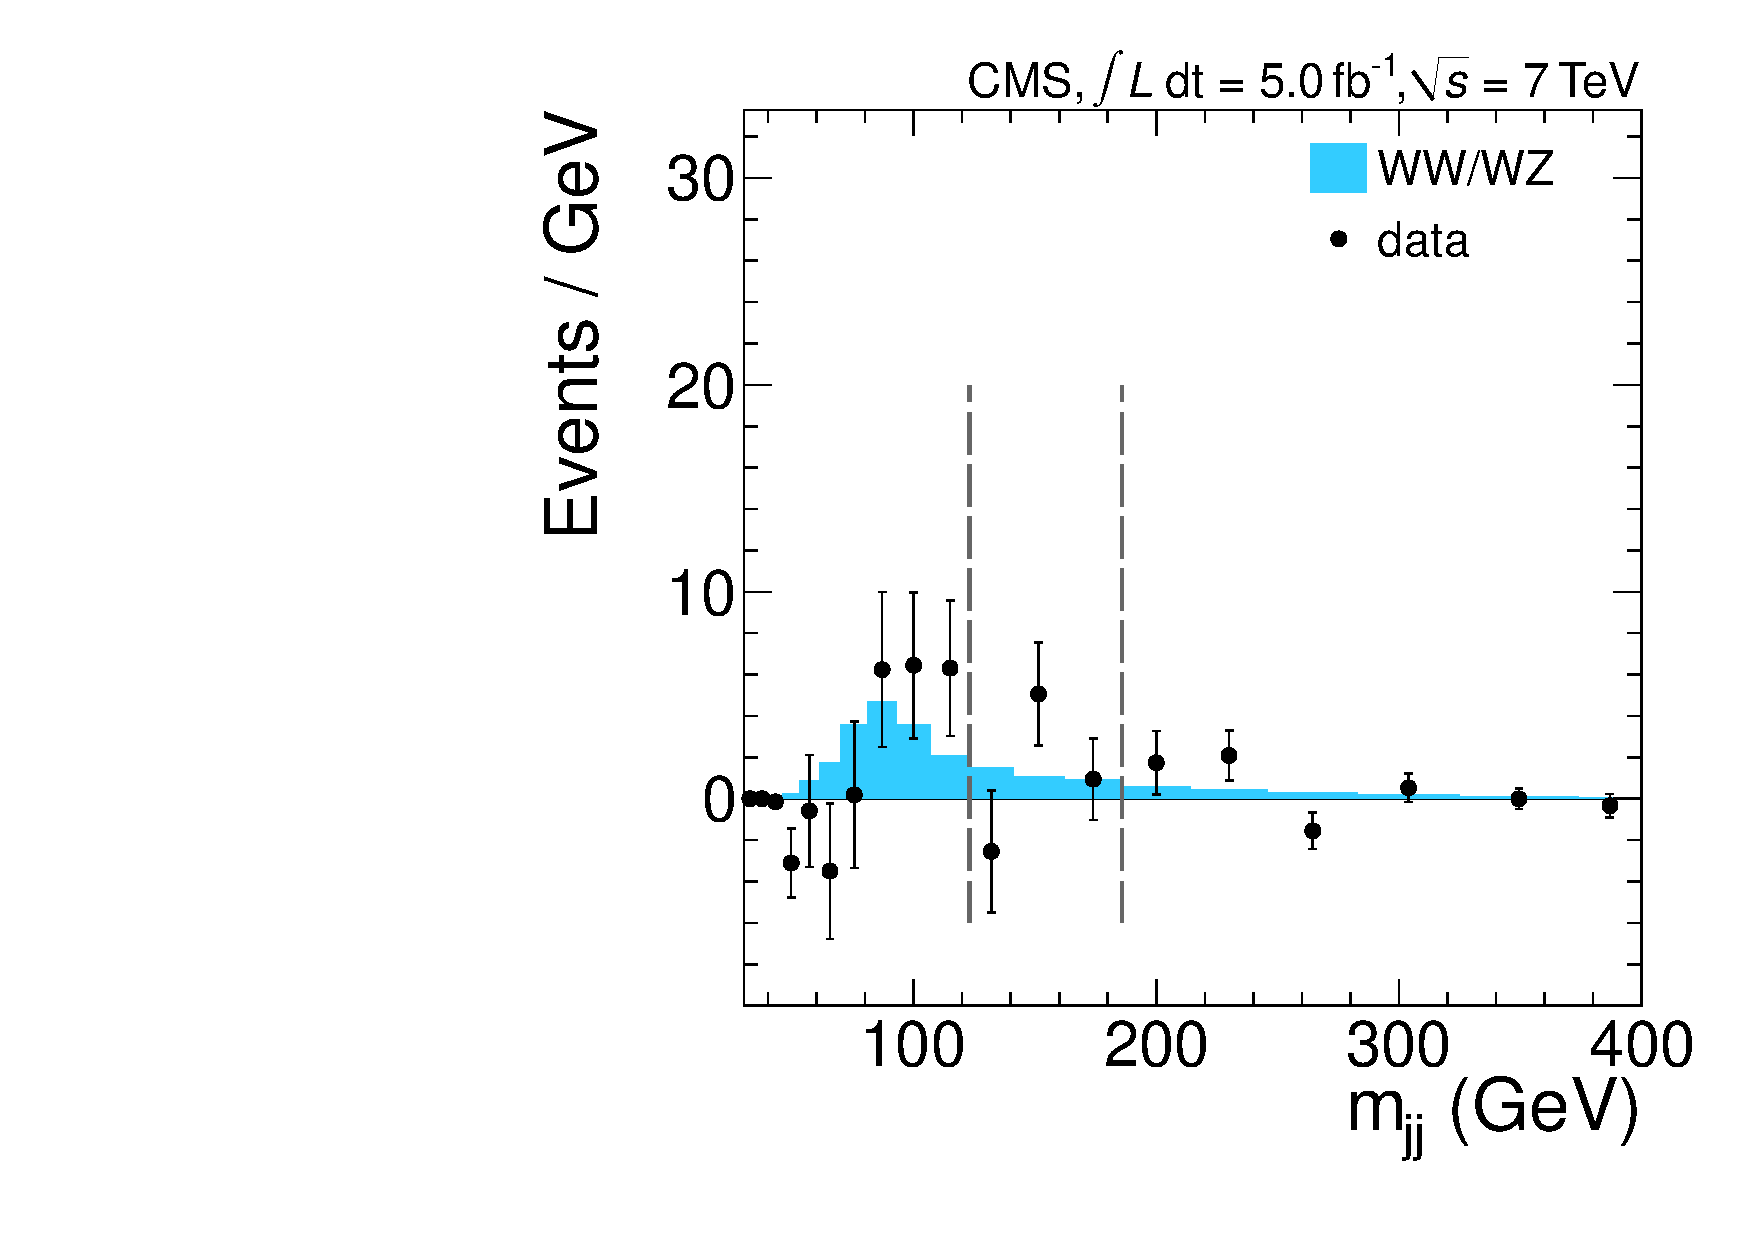
\includegraphics[width=0.49\textwidth]{figs/mjjfit_3jetsample/Wjj_Mjj_Muon_3jets_Subtracted.pdf}
    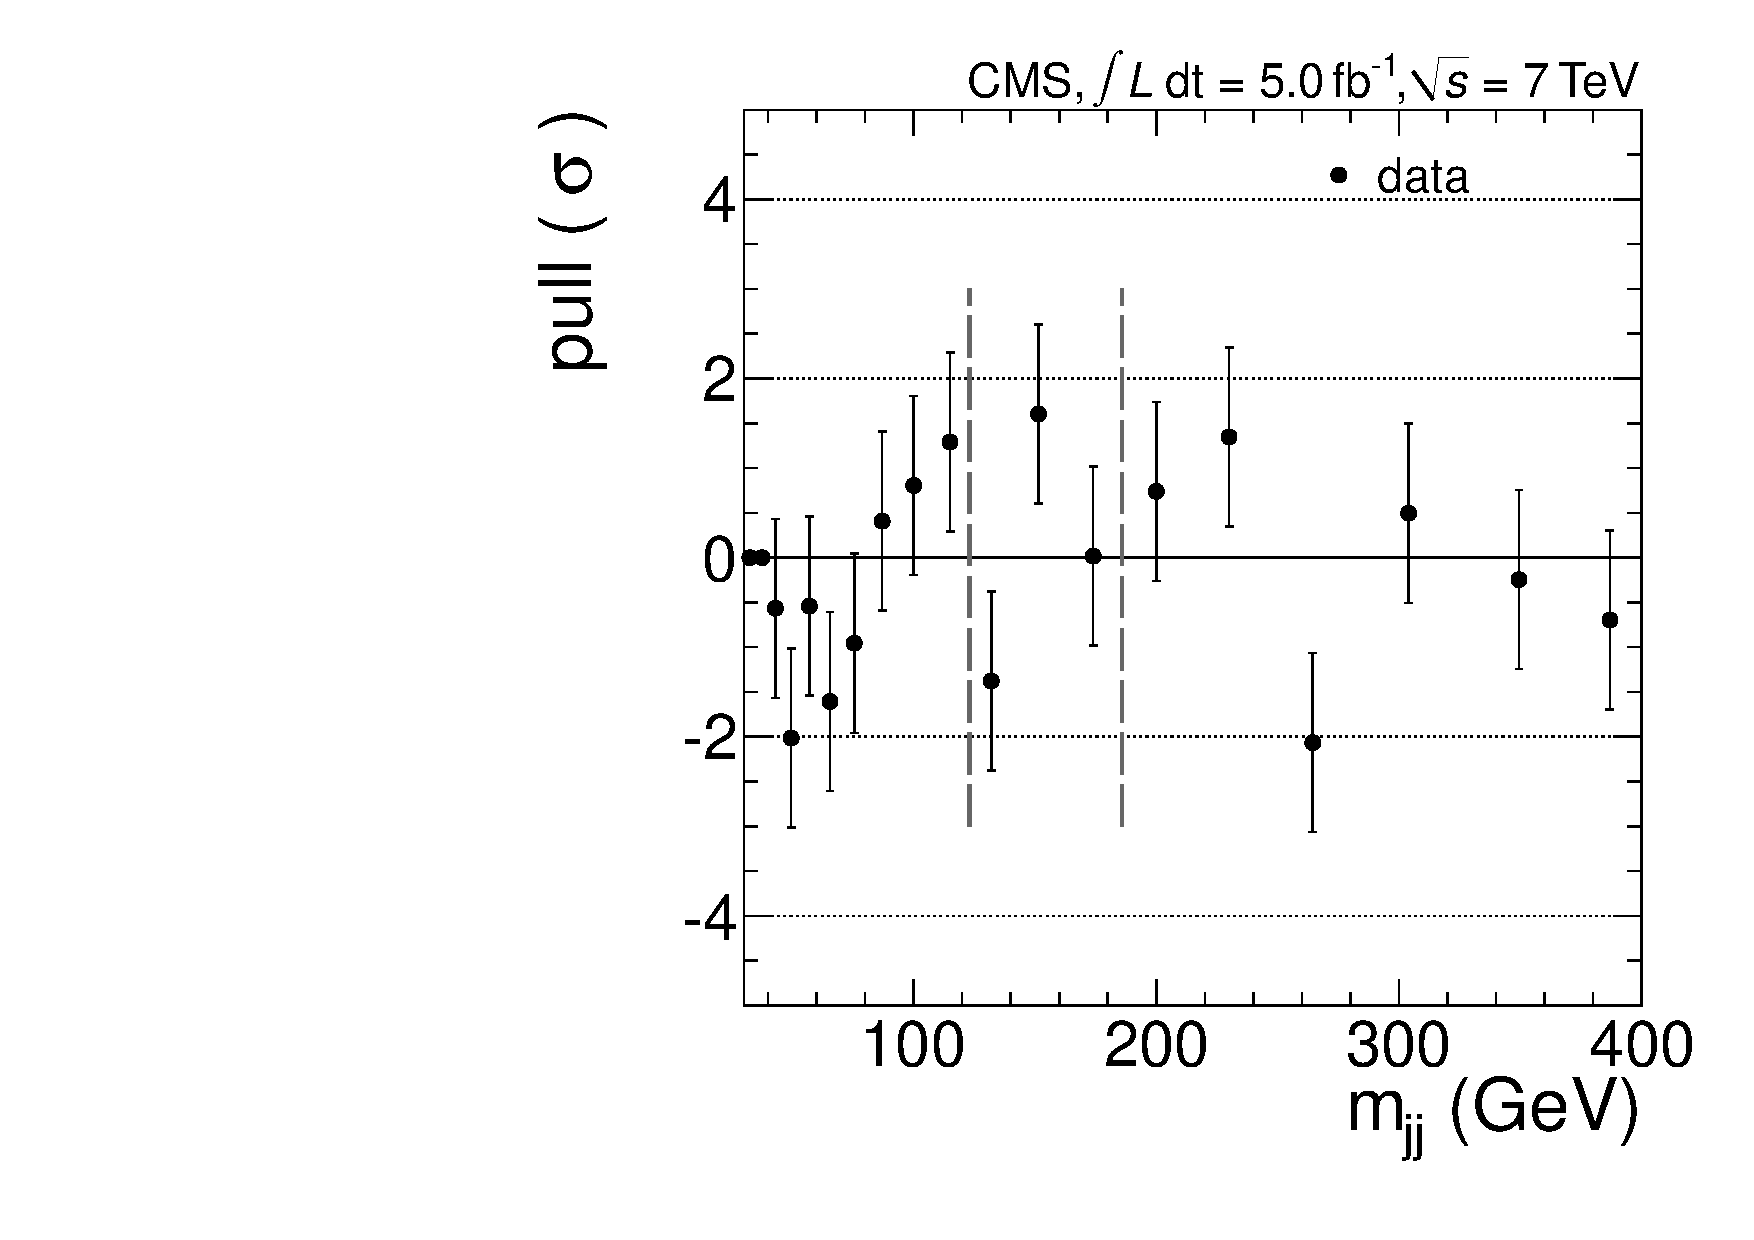
\includegraphics[width=0.49\textwidth]{figs/mjjfit_3jetsample/Wjj_Mjj_Muon_3jets_Pull.pdf}
    \caption{Distribution of the dijet invariant mass for the 3-jet events in muon data and Monte Carlo: 
      (upper left) All background components stacked together, 
      (upper right) unstacked, (lower left) [Data minus all backgrounds except diboson],  
      (lower right) normalized residual between data and MC. The vertical dotted lines
      indicate the mass interval excluded from the fit.}
    \label{fig:mjj_3jet_mu}}
\end{figure}
%%%%%%%%%%%%%%%%%%%%
%%%%%%%%%%%%%%%%%%%%
\begin{figure}[h!]
  {\centering

    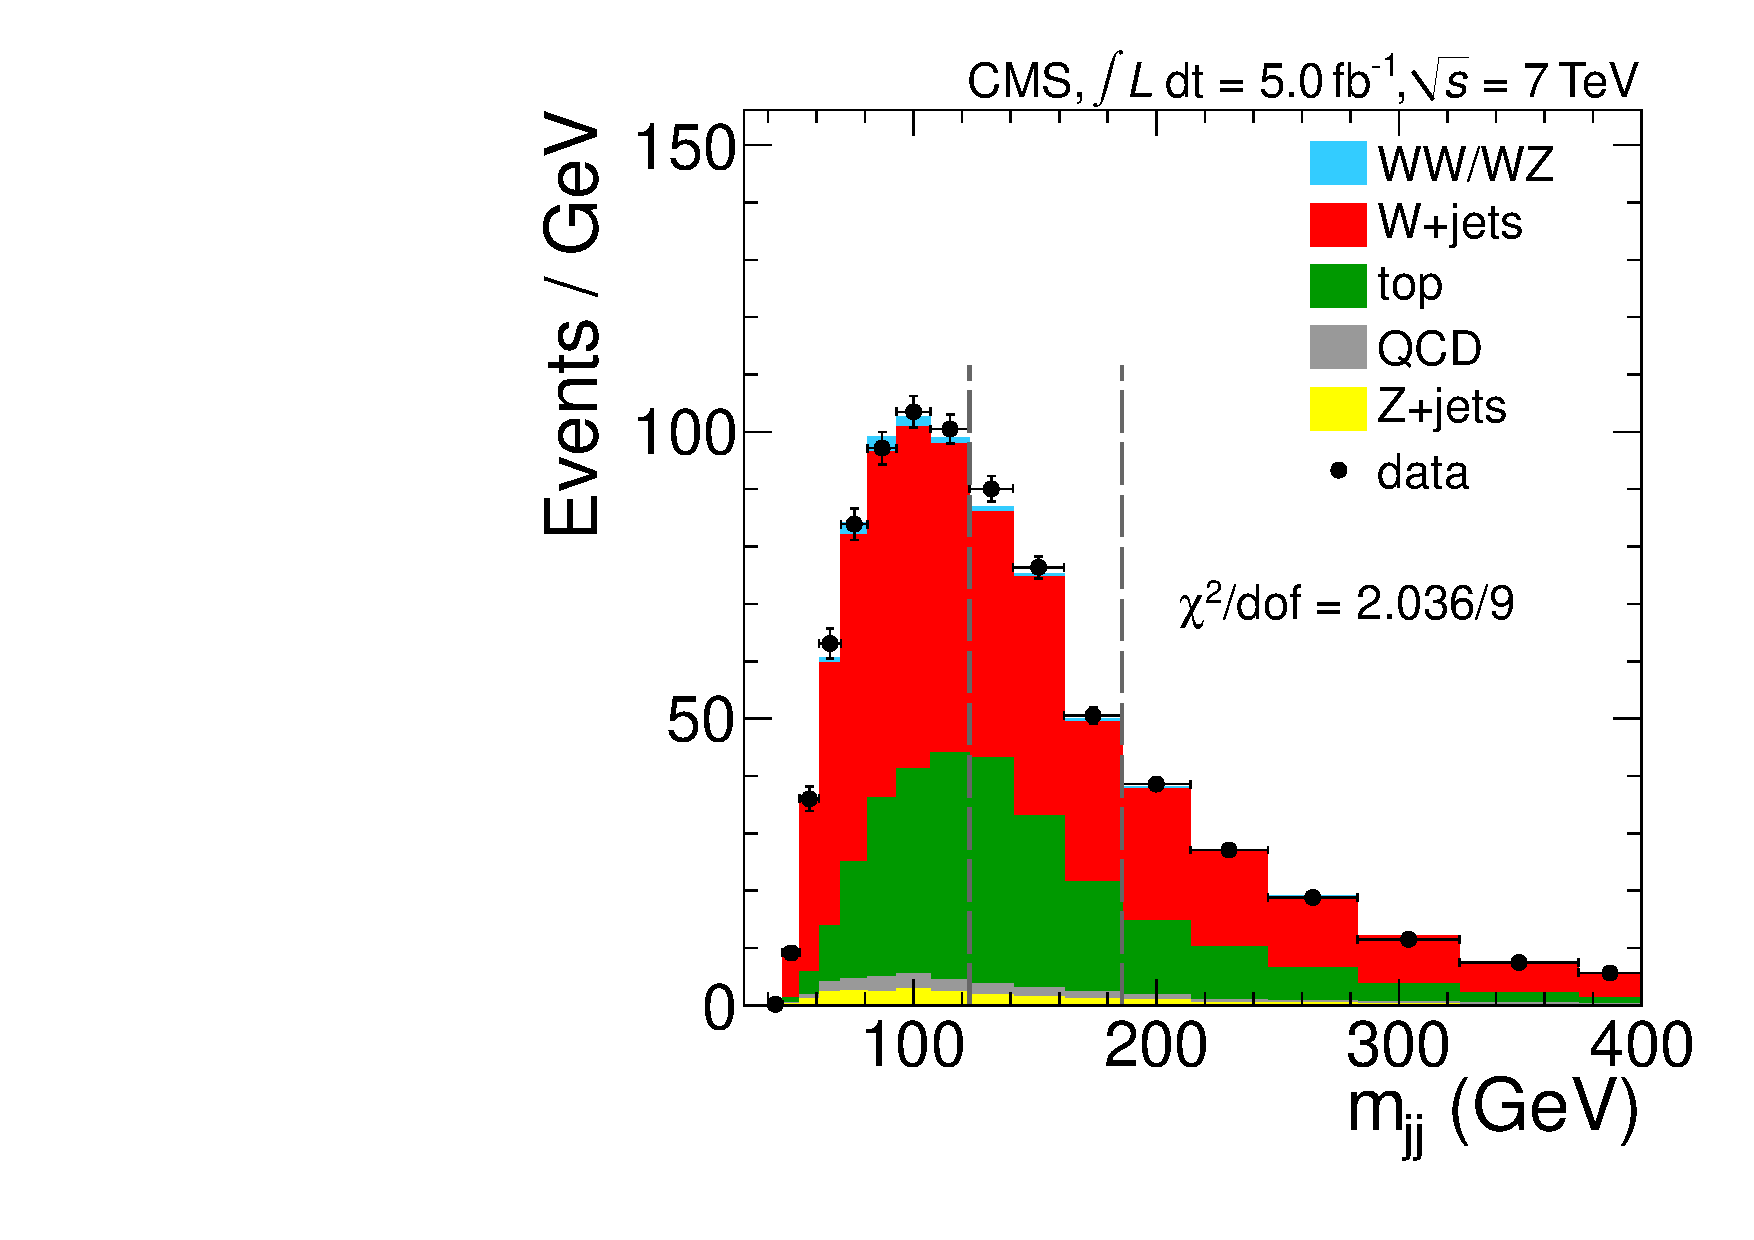
\includegraphics[width=0.49\textwidth]{figs/mjjfit_3jetsample/Wjj_Mjj_Electron_3jets_Stacked.pdf}
    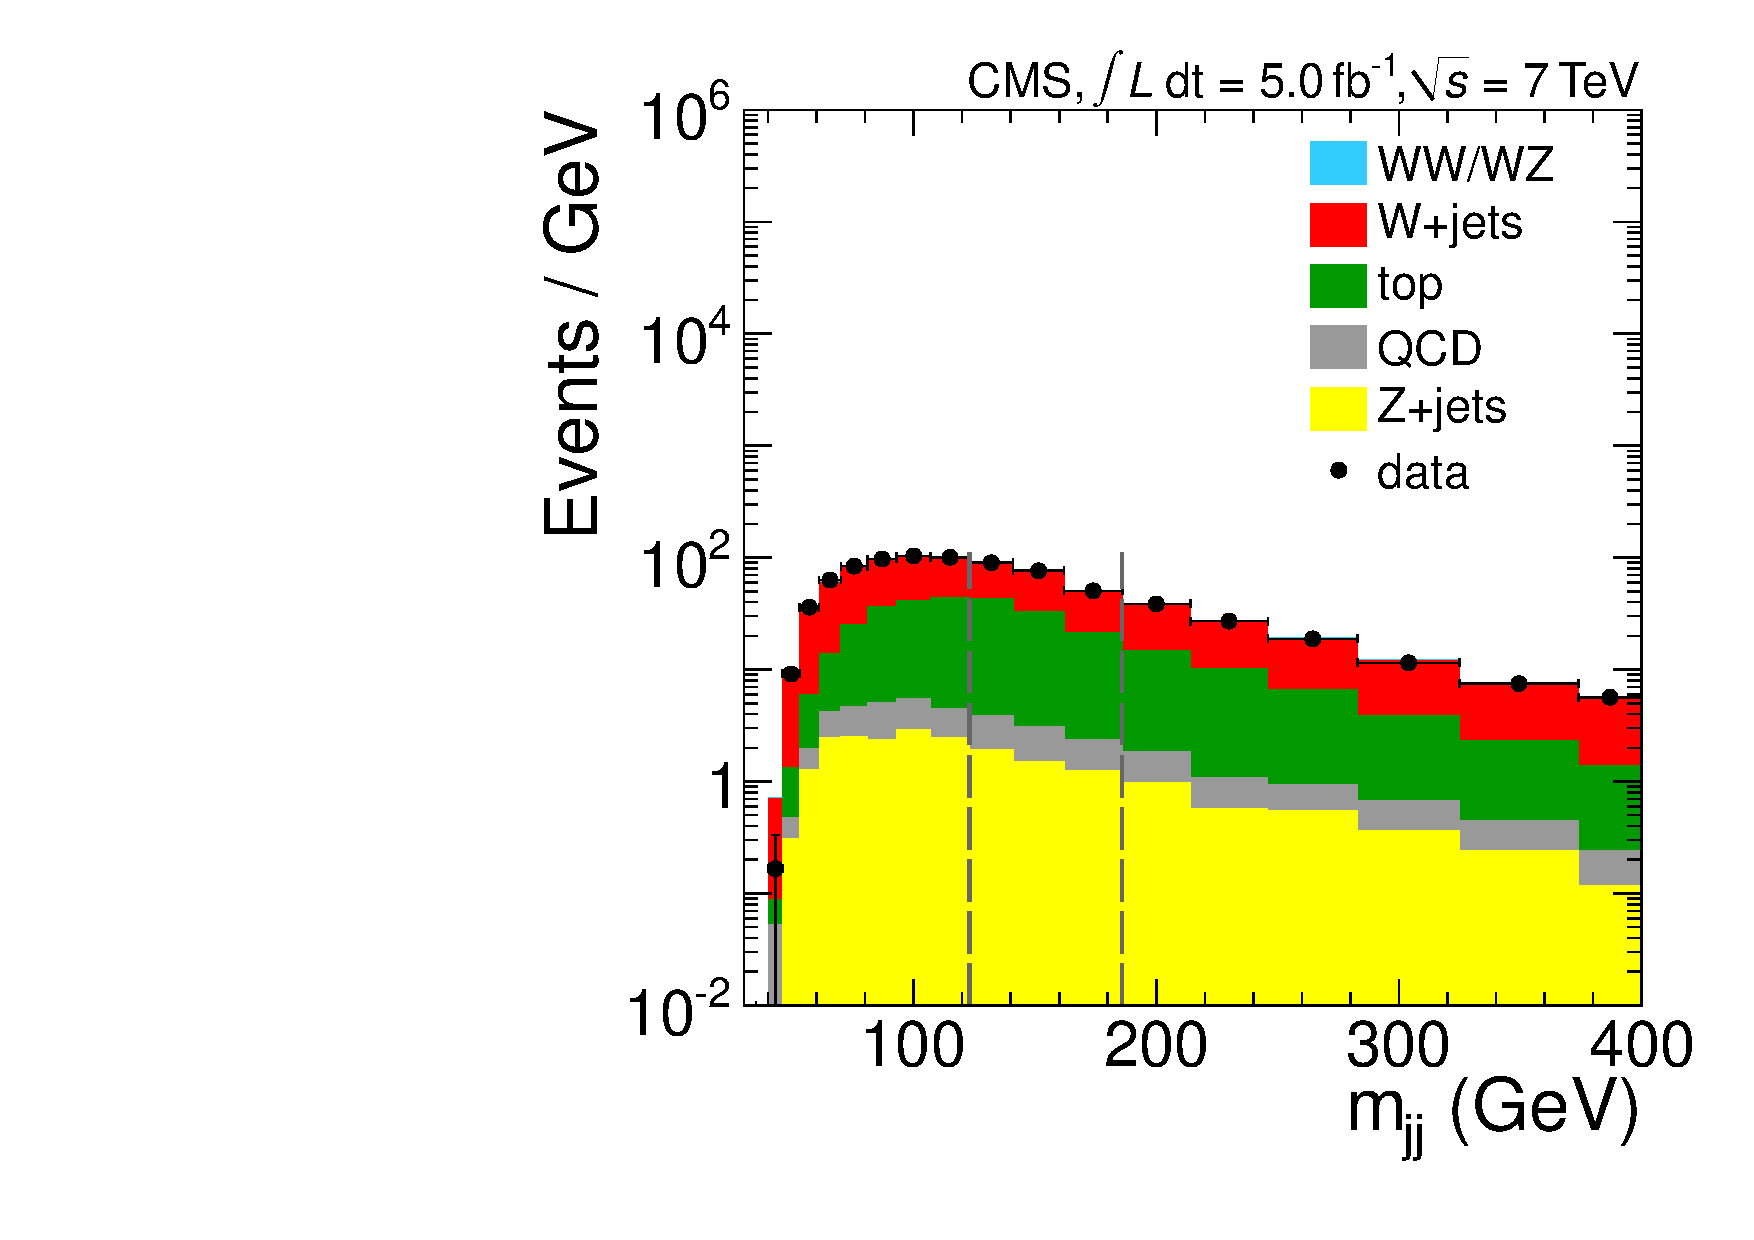
\includegraphics[width=0.49\textwidth]{figs/mjjfit_3jetsample/Wjj_Mjj_Electron_3jets_Stacked_log.pdf}
    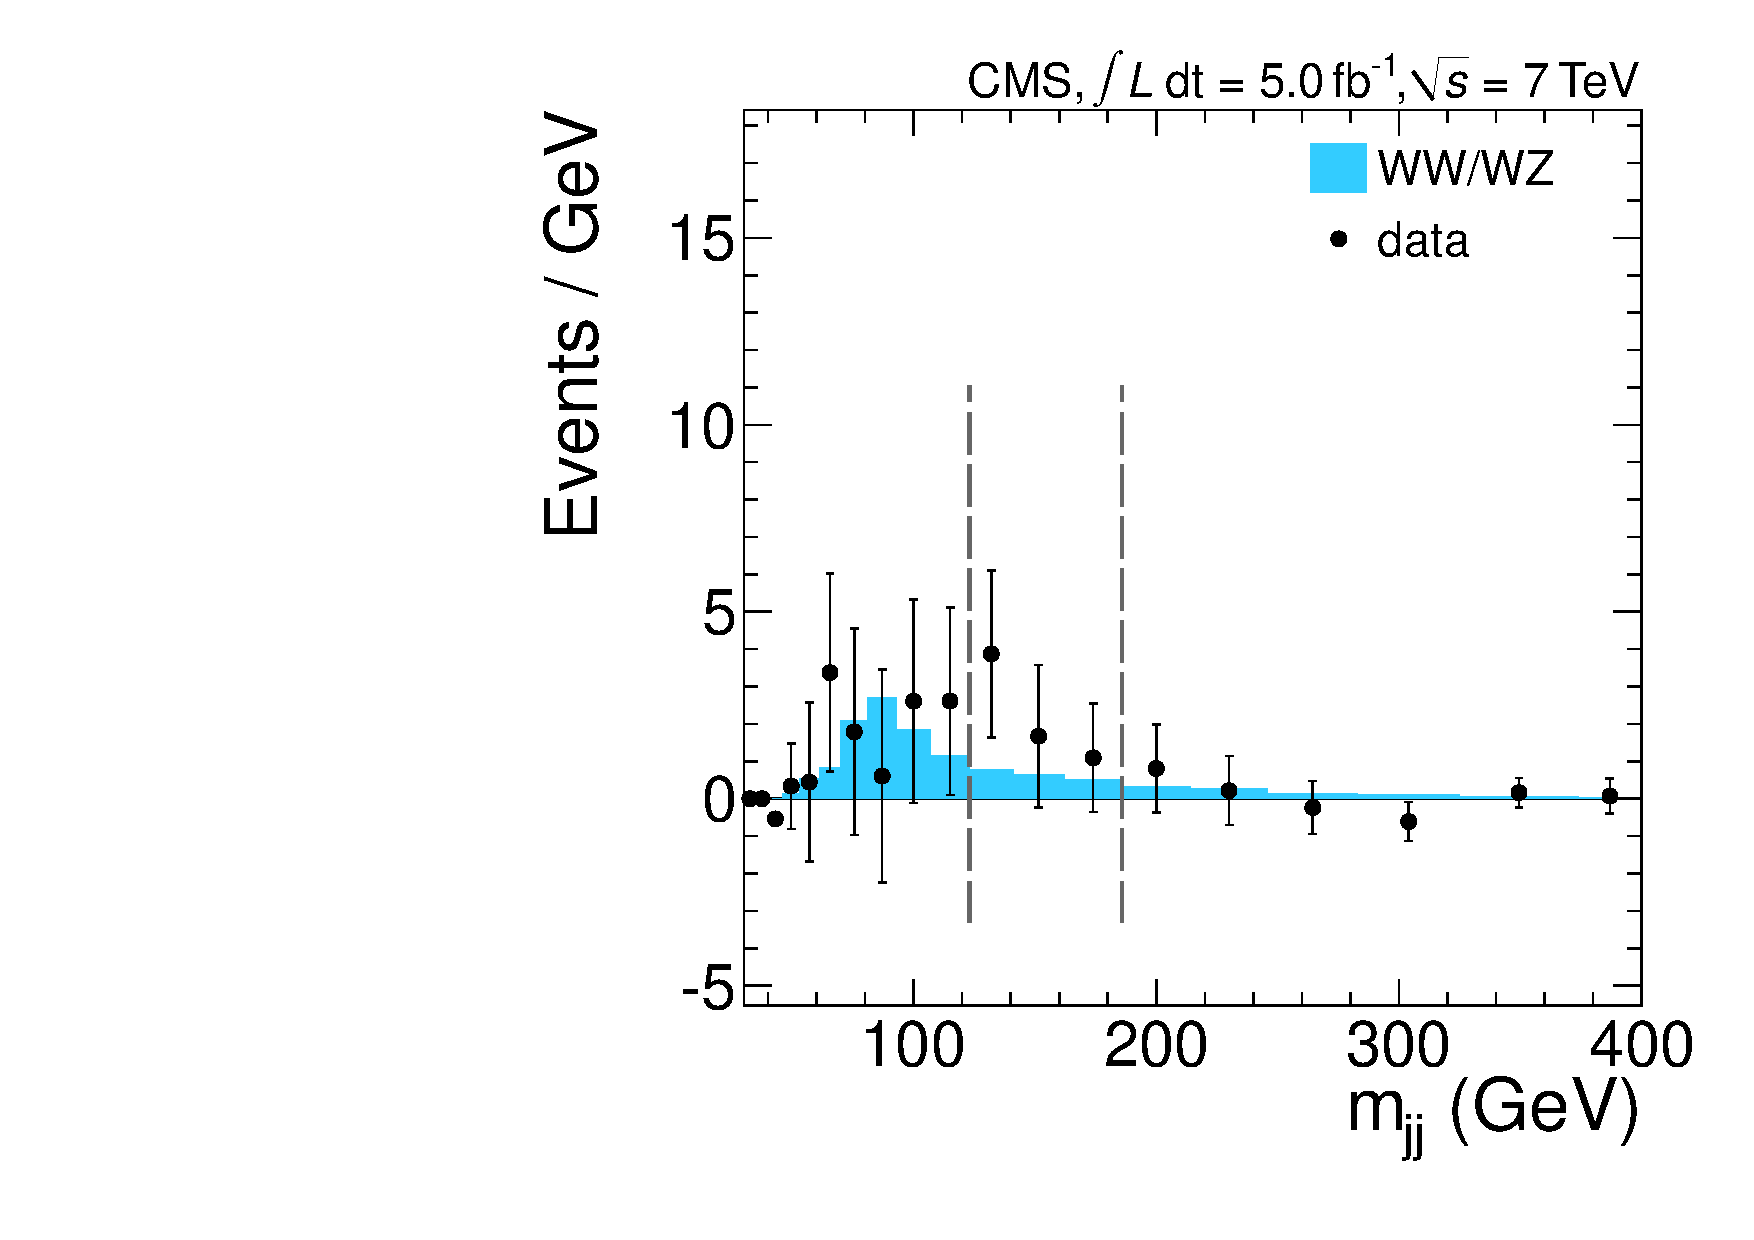
\includegraphics[width=0.49\textwidth]{figs/mjjfit_3jetsample/Wjj_Mjj_Electron_3jets_Subtracted.pdf}
    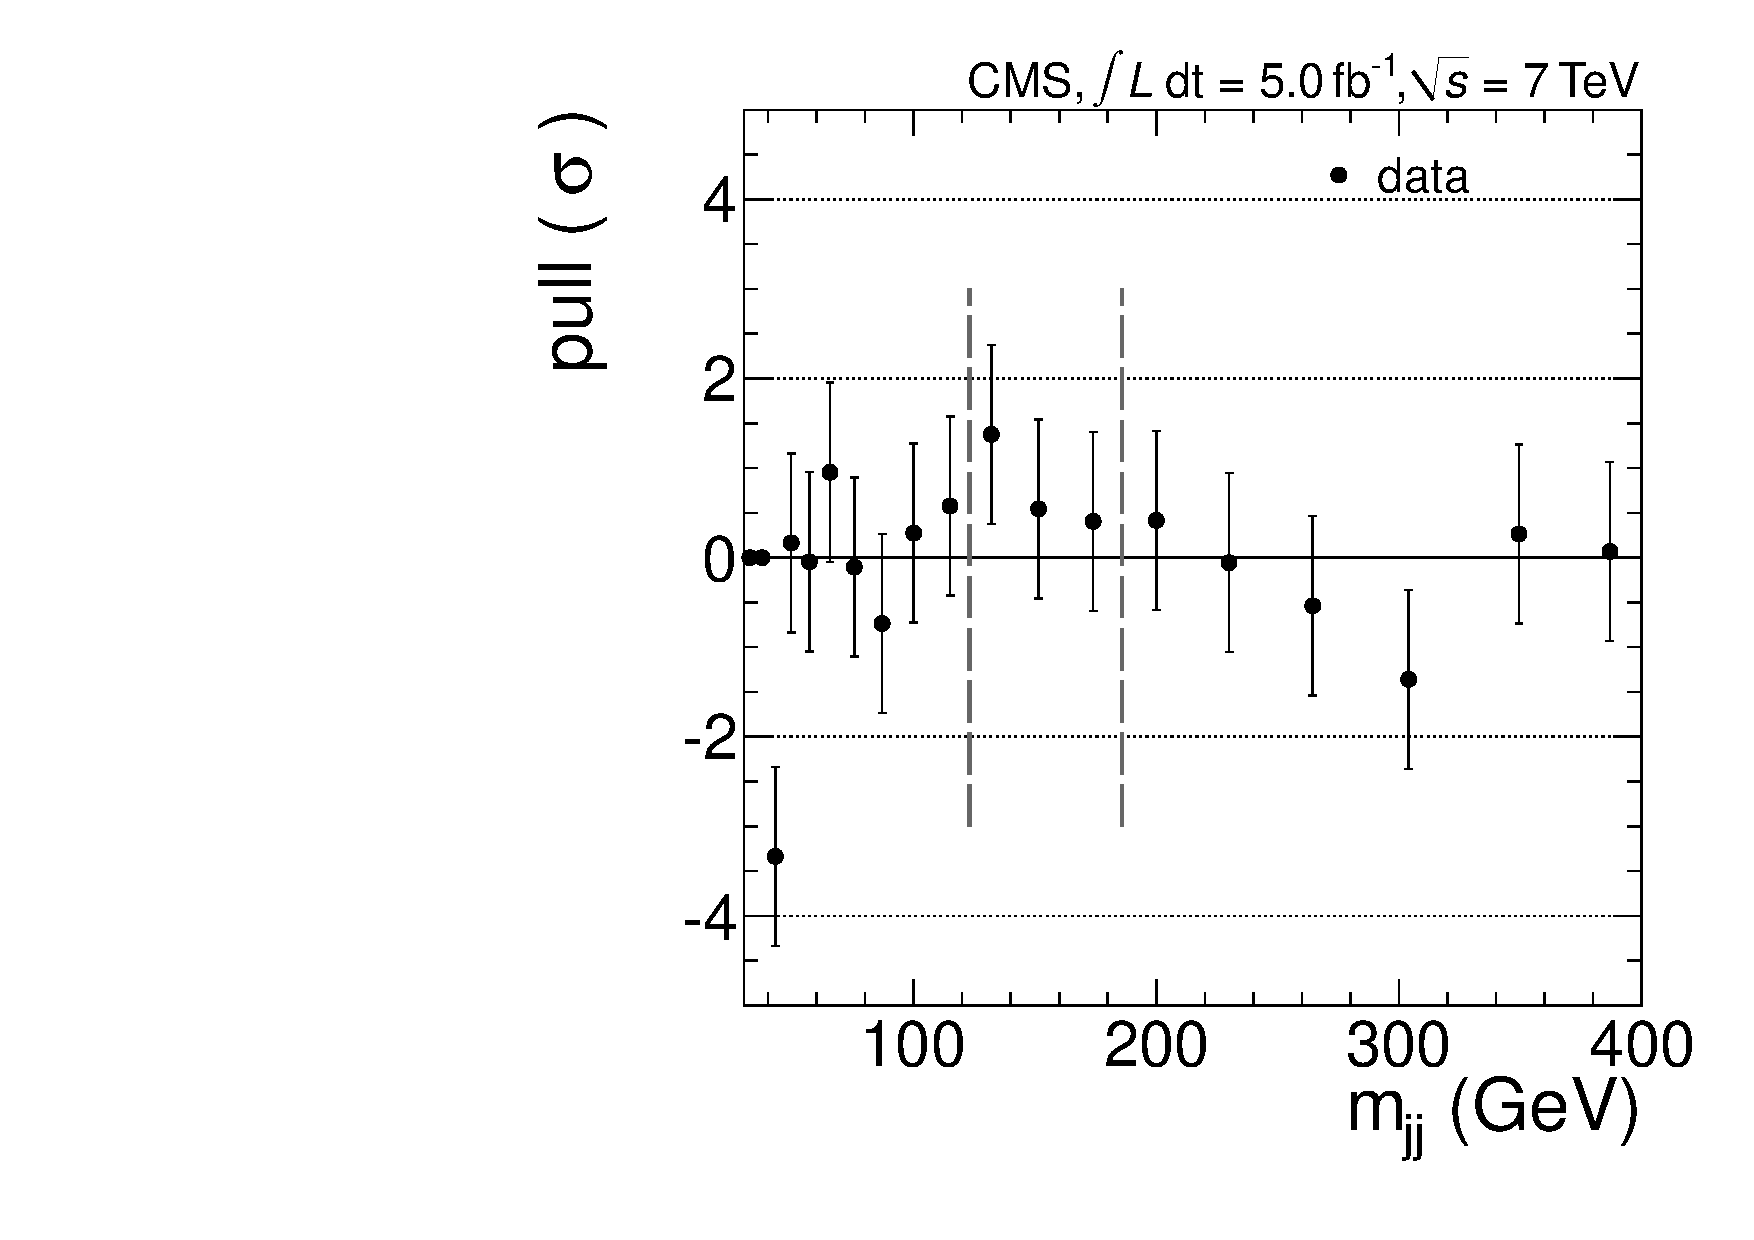
\includegraphics[width=0.49\textwidth]{figs/mjjfit_3jetsample/Wjj_Mjj_Electron_3jets_Pull.pdf}
    \caption{Distribution of the dijet invariant mass for the 3-jet events in electron data and Monte Carlo: 
      (upper left) All background components stacked together, 
      (upper right) unstacked, (lower left) [Data minus all backgrounds except diboson],  
      (lower right) normalized residual between data and MC. The vertical dotted lines
      indicate the mass interval excluded from the fit.}
    \label{fig:mjj_3jet_el}}
\end{figure}
%%%%%%%%%%%%%%%%%%%%
%%%%%%%%%%%%%%%%%%%%
%\begin{figure}[h!t]
%  {\centering
%    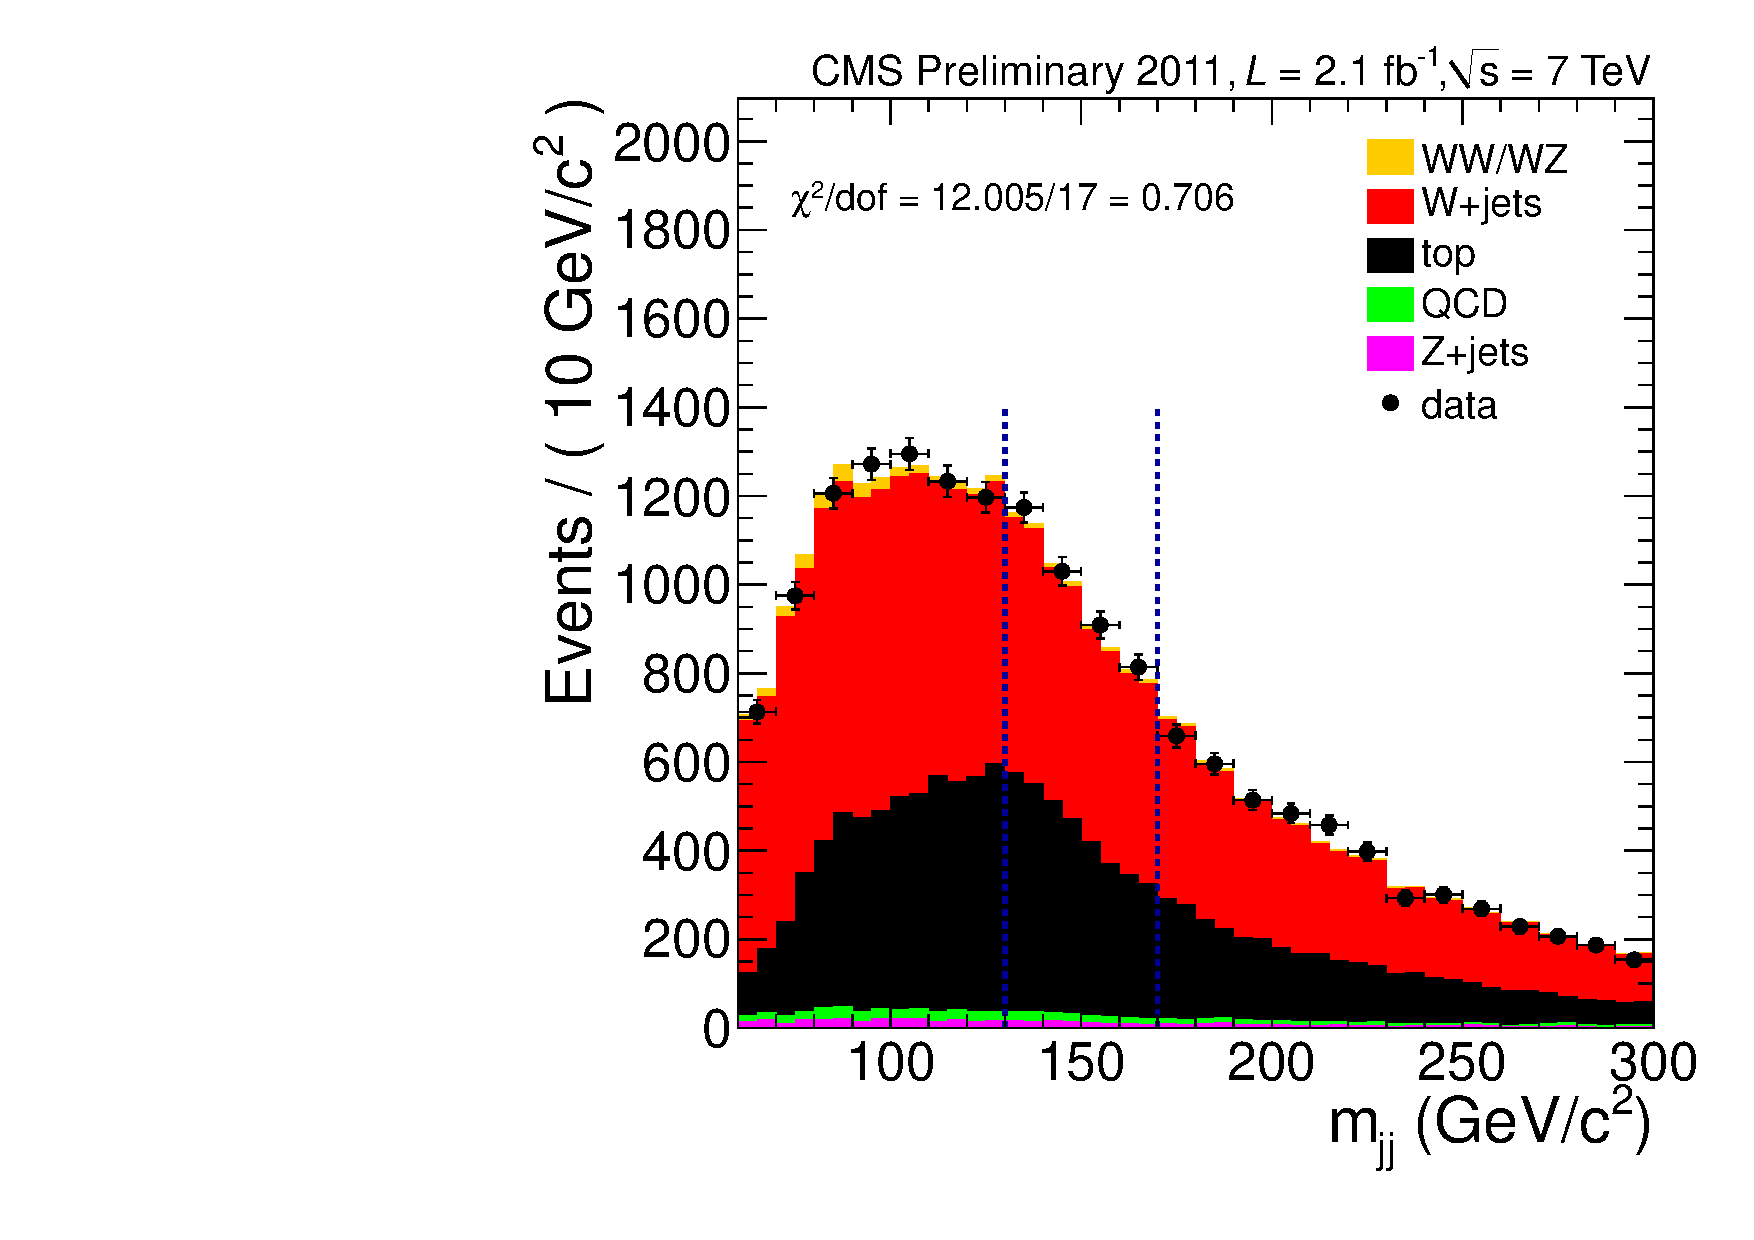
\includegraphics[width=0.49\textwidth]{figs/mjjfit_3jetsample/Wjj_Mjj_3jets_Stacked.pdf}
%    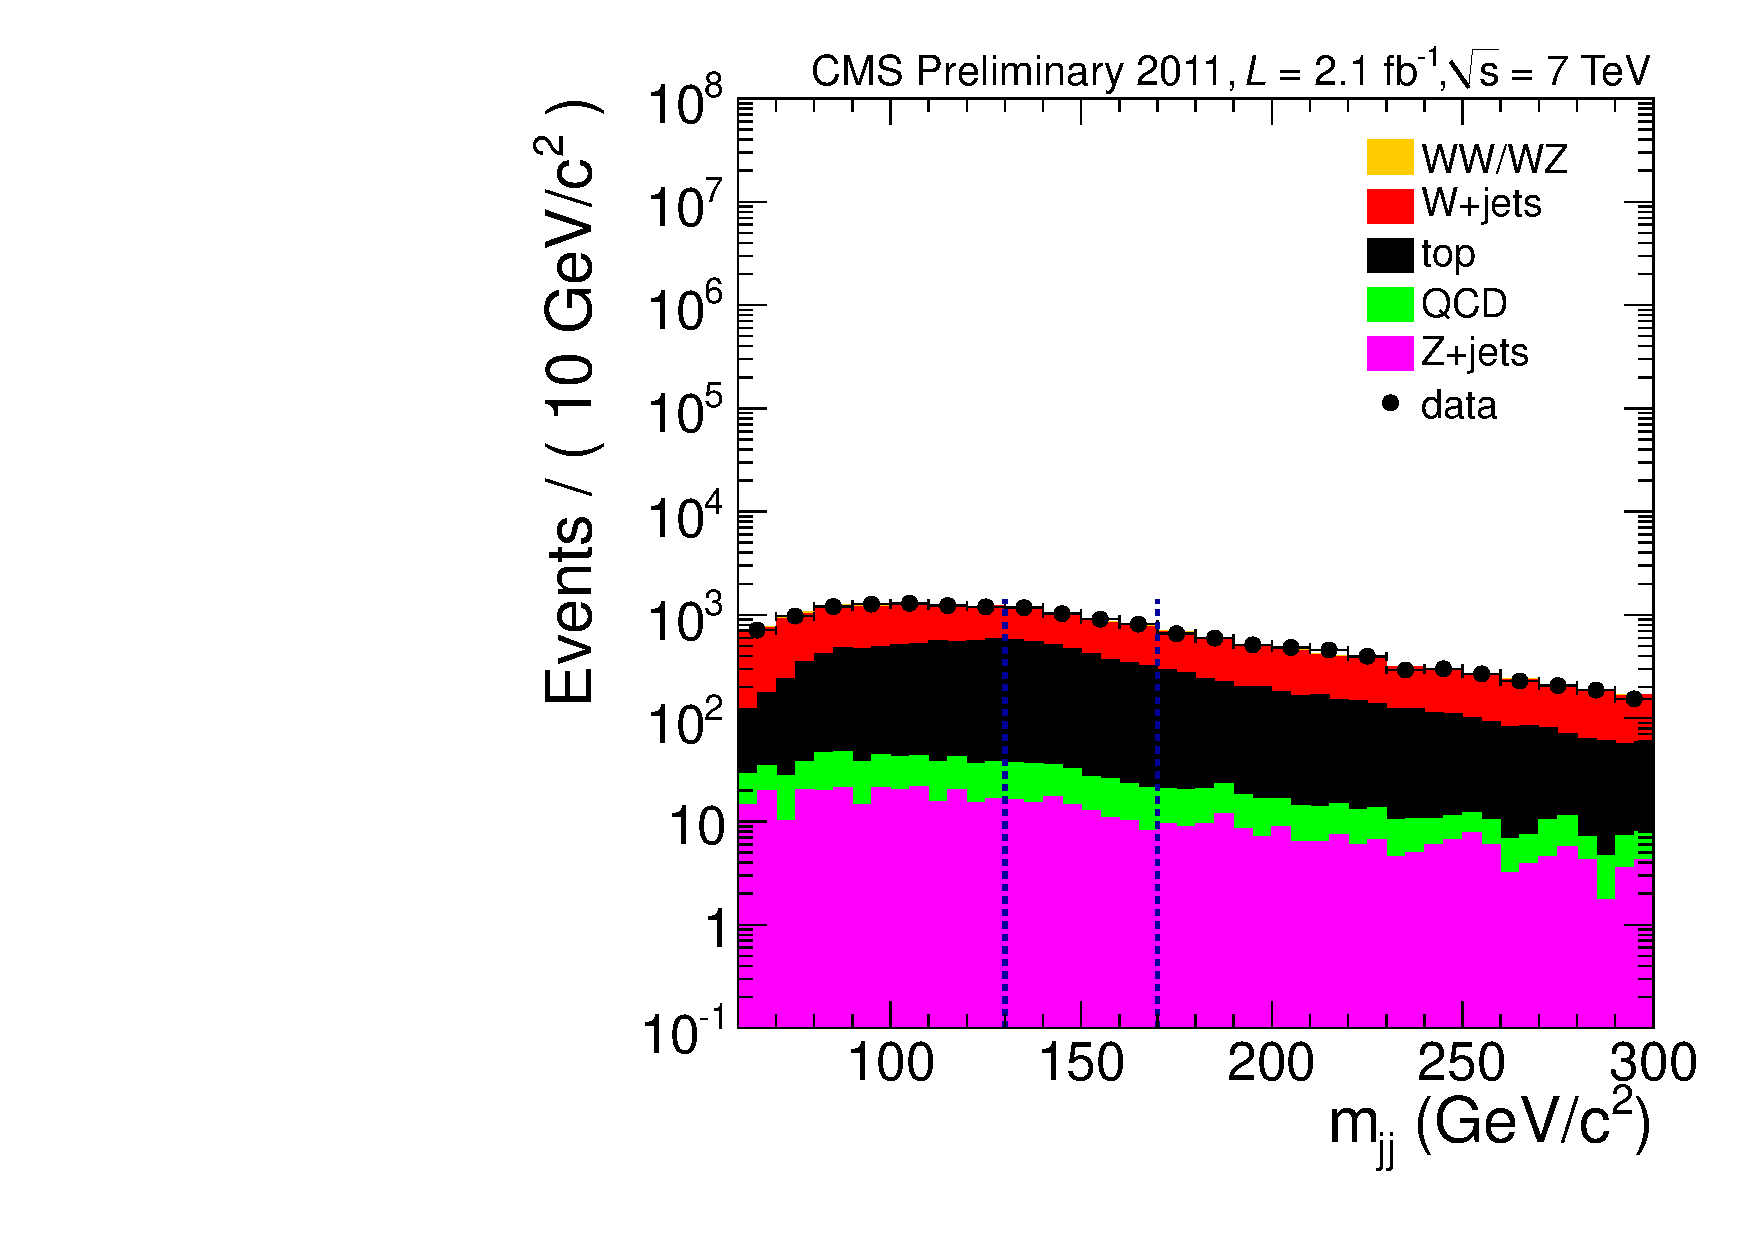
\includegraphics[width=0.49\textwidth]{figs/mjjfit_3jetsample/Wjj_Mjj_3jets_Stacked_log.pdf}
%    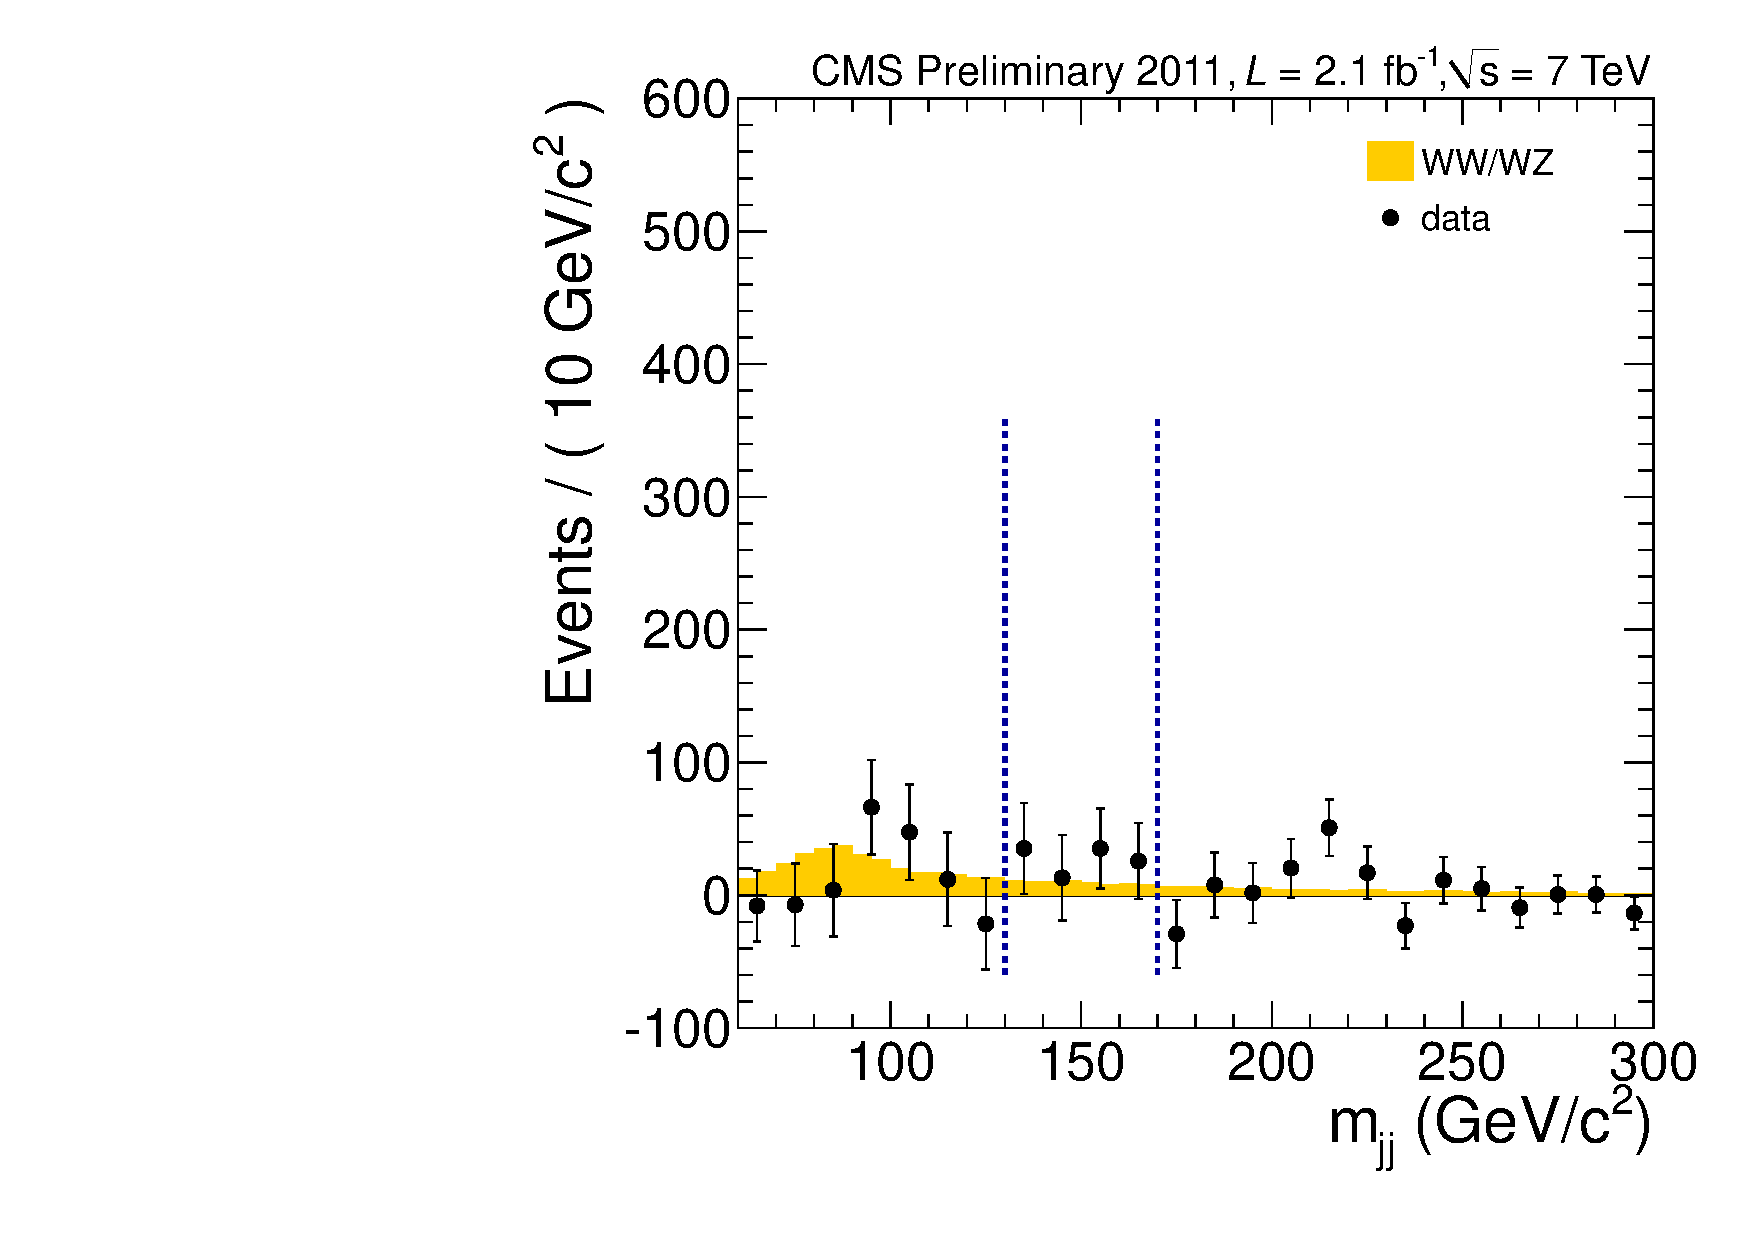
\includegraphics[width=0.49\textwidth]{figs/mjjfit_3jetsample/Wjj_Mjj_3jets_Subtracted.pdf}
%    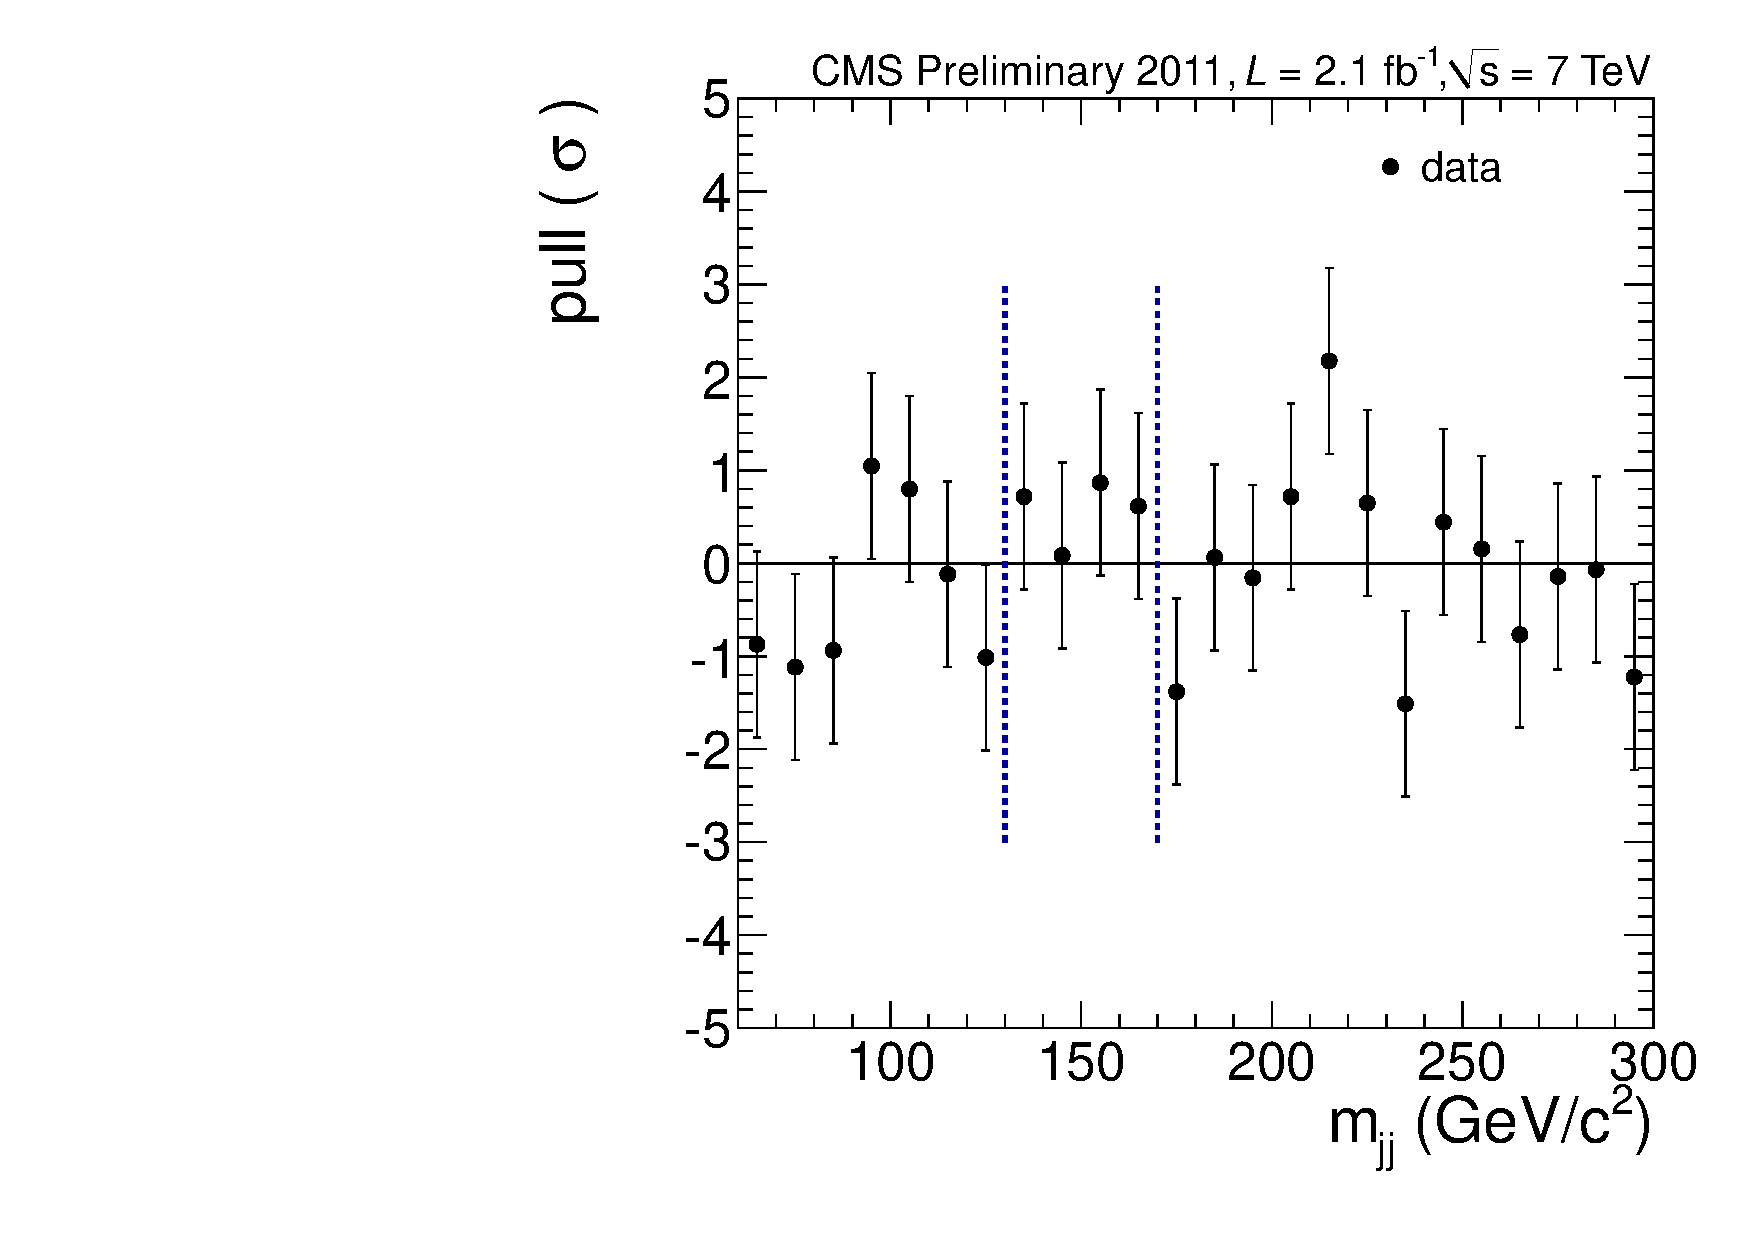
\includegraphics[width=0.49\textwidth]{figs/mjjfit_3jetsample/Wjj_Mjj_3jets_Pull.pdf}
%    \caption{Distribution of the dijet invariant mass for the 3-jet events in data and Monte Carlo: 
%      (upper left) All background components stacked together, 
%      (upper right) unstacked, (lower left) [Data minus all backgrounds except diboson],  
%      (lower right) normalized residual between data and MC. The vertical dotted lines
%      indicate the mass interval excluded from the fit.}
%    \label{fig:mjj_3jet}}
%\end{figure}
%%%%%%%%%%%%%%%%%%%%
\clearpage
%%%%%%%%%%%%%%%%%%%%%%%%%%%%%%%%%%%%%%%%%%%%%%%%%%%%%%%%%%%%
%%%%%%%%%%%%%%%%%%%%%%%%%%%%%%%%%%%%%%%%%%%%%%%%%%%%%%%%%%%%
%\subsection{Fit results for the muon channel only}
%\label{sec:mjj_fit_mu}
%\clearpage
%%%%%%%%%%%%%%%%%%%%%%%%%%%%%%%%%%%%%%%%%%%%%%%%%%%%%%%%%%%%
%%%%%%%%%%%%%%%%%%%%%%%%%%%%%%%%%%%%%%%%%%%%%%%%%%%%%%%%%%%%
%\subsection{Fit results for the electron channel only}
%\label{sec:mjj_fit_ele}
%\clearpage
%%%%%%%%%%%%%%%%%%%%%%%%%%%%%%%%%%%%%%%%%%%%%%%%%%%%%%%%%%%%
%%%%%%%%%%%%%%%%%%%%%%%%%%%%%%%%%%%%%%%%%%%%%%%%%%%%%%%%%%%%
%--------------------------------------------------
\subsection{Fit Validation}

We verify that the signal extraction procedure is unbiased and that 
statistical uncertainties reported have good coverage by constructing
and fitting toy datasets. Since our fit procedure is the same in both
electron and muon channels, we validate it for muons, where the trigger
efficiency corrections as well as the kinematic turn-on curve are
better understood. The specific steps are:
\begin{enumerate}
\item Perform the default fit and obtain the expected yields 
(Table~\ref{table:FitValidation_input}).
\item Generate toy Monte Carlo for each process from the corresponding MC distributions.
\item Construct 1000 sample datasets. Take correlations (between expected yields) into 
account and implement smearing by Fit and Poisson errors.
\item Perform the fit for each sample dataset.
\item Examine the resultant Yields and Pulls.
\end{enumerate}


\subsubsection{Expected Event Generation}
Due to the constraints imposed by the data the fitted event yields are strongly correlated
(Secs.~\ref{sec:mjj_2jetfit},~\ref{sec:mjj_3jetfit}). This fact must be taken into account 
when smearing the expected values by the fit errors. Thus we perform a transformation to 
the coordinate system where the yields are uncorrelated, smear and transform back. Namely,
for each toy dataset we:
\begin{enumerate}
\item Diagonalize the Covariance Matrix ($\Sigma$). I.e. find $M$ such that $M\Sigma M^{-1}$ is 
diagonal (Rows of $M$ are in fact the eigenvectors of $\Sigma$).
\item Generate the errors $z_i$: throw the random events with $\sigma_i^2=(M\Sigma M^{-1})_{ii}$ 
and mean=$0$.
\item Transform back: $x_i=\mu_i+(M^{-1}Z)_i$ ($\mu$ is the expected value from the default fit).
\item Poisson-smear $x_i$ and generate the dataset.
\item Perform the fit.
\end{enumerate}
Also note that the error on the sum of the yields is given by the sum of all of the elements
in the covariance matrix.


\subsubsection{Results}
Similarly to the default fit, we perform the validation for the 2- and
3-jet bins independently. The fitted parameter values are shown in
Figs~\ref{fig:Validation_Yields_2j},~\ref{fig:Validation_Yields_3j},
and gaussian fits to the distributions are summarized in
Table~\ref{table:FitValidation_Yields_results}. Note that there is
substantial variation in the gaussian widths due to differing
constraints imposed when fitting
(Table~\ref{tab:mjj_shapes_and_normalization}).  Overall, there is a
$-650$ event bias for $t\bar{t}$ and a $+690$ event bias for W+jets in
the 3-jet bin, due to a strong correlation between the two. The rest
of the yields returned by the fitter are consistent with the
expectation within a few percent ( or $<30$ events).

Likewise, pull distributions are shown in
Figs~\ref{fig:Validation_Pulls_2j},~\ref{fig:Validation_Pulls_3j}, and
gaussian fits to them are summarized in
Table~\ref{table:FitValidation_Pulls_results}. The initial gaussian
constraint dominates the errors after the fit is performed (often
times almost entirely). Plus, limited sensitivity to individual yields
leads to a relatively small spread and narrow ($\sigma<1$) Pull
Distributions. The effect propagates to the W+jets, where
$\sigma_{Pull-2J}=0.838\pm 0.019$.

The expected values and pulls for the fraction of Matrix Element -
Parton Shower Matching MC ($fMU$) and fraction of Factorization Scale
MC ($fSU$) in the W+jets sample are displayed in
Figs~\ref{fig:Validation_fMUfSU_2j}, ~\ref{fig:Validation_fMUfSU_3j}.
As usual, $fMU<0$ ($fSU<0$) denotes the fact that we're using a
Matching Down (Scale Down) sample instead; which can lead to different
(pull and yield) distributions when these fractions are $>0$ vs
$<0$. Furthermore, insufficient discriminating ability between Up and
Down templates (shown in
Fig~\ref{fig:Validation_fMUfSU_ShapeComparisonUpVsDown}) has
previously led to bifurcated ({\it i.e.} clustered around two
different points) values for the fractions. %({\it e.g.}
%Fig~\ref{fig:WjetsTemplateQ2MatchingScan}). 
The impact is seen in the pull as well as (to a lesser extend) the
expected value distributions, and can explain the tail in the W+jets
Pull (Fig.~\ref{fig:Validation_Pulls_3j}e) ).

The Total Yields and Pulls are shown in
Fig.~\ref{fig:Validation_Total_YieldsAndPulls}.  The distributions are
Gaussian and centered near $0$. Pull $\sigma$ is somewhat
overestimated due to lack of sensitivity in the fitter ({\it e.g.}
difficulties fitting for $fMU$, $fSU$), while the Yield bias is less
than $0.15\%$. %In the end, our results are consistent with the
%expectations and observations from other studies.


%%%%%%%%%%%%%%%%%%%%%%%%%%%%
%%%%%%%
\begin{table}[tb]
\caption{Parameter Values used as inputs to generate pseudo experiments for the muon fit validation studies.}
\begin{center}
\begin{tabular}{|c|c|c|}
\hline
   Process           & 2-Jet bin & 3-Jet bin \cr \hline
\vspace{-0.5cm} & & \cr
N{Diboson}            &      1213   &  302  \cr \hline
N{W+jets}             &       46283 & 11263 \cr \hline
N{QCD}                &         79  &   23  \cr \hline
N{$t\bar{t}$}         &      3700   & 7275  \cr \hline
N{SingleTop}          &       144   &  829  \cr \hline
N{Z+jets}             &       1225  &  385  \cr \hline
$fMU$                 &       0.25  & 0.18  \cr \hline
$fSU$                 &       0.36  & 0.08  \cr \hline
\end{tabular}
\end{center}
\label{table:FitValidation_input}
\end{table}
%%%%%%%
%%%%%%%
\begin{table}[tb]
\caption{Parameter Fit Summary}
\begin{center}
\begin{tabular}{|c|c|c|c|c|}
\hline
   Parameter (Fitted-Expected)
 & 2-Jet Mean
 & 2-Jet $\sigma$
 & 3-Jet Mean
 & 3-Jet $\sigma$ \cr
\hline
\vspace{-0.5cm} & & \cr
{Diboson} & $-25.9\pm 2.4$ & $71.8\pm 1.7$ & $-1.4\pm 0.2$ & $5.7\pm 0.1$ \cr
\hline
{W+jets} & $85.2\pm 12.9$ & $378.4\pm 10.2$ & $686.6\pm 13.3$ & $359.1\pm 10.3$ \cr 
\hline
{Z+jets} & $0.05\pm 0.03$ & $0.81\pm 0.02$ & $-0.37\pm 0.01$ & $0.31\pm 0.01$ \cr 
\hline
{QCD} & $9.9\pm 0.8$ & $24.3\pm 0.6$ & $-13.7\pm 0.3$ & $8.2\pm 0.2$ \cr 
\hline
{$t\bar{t}$} & $-26.4\pm 1.3$ & $38.4\pm 0.9$ & $-654.5\pm 7.0$ & $218.9\pm 5.2$ \cr 
\hline
{SingleTop} & $-1.6\pm 0.1$ & $2.7\pm 0.1$ & $-6.1\pm 0.1$ & $2.3\pm 0.1$ \cr 
\hline
{$fMU$} & $-0.01\pm 0.00$ & $0.13\pm 0.00$ & $0.01\pm 0.00$ & $0.12\pm 0.00$ \cr
\hline
{$fSU$} & $-0.12\pm 0.00$ & $0.12\pm 0.00$ & $0.12\pm 0.00$ & $0.11\pm 0.00$ \cr
\hline
\end{tabular}
\end{center}
\label{table:FitValidation_Yields_results}
\end{table}
%%%%%%%
%%%%%%%
\begin{table}[tb]
\caption{Fit Pull Summary}
\begin{center}
\begin{tabular}{|c|c|c|c|c|}
\hline
   Parameter
 & 2-Jet Pull
 & 2-Jet $\sigma_{Pull}$
 & 3-Jet Pull
 & 3-Jet $\sigma_{Pull}$ \cr
\hline
\vspace{-0.5cm} & & \cr
{Diboson} & $-0.17\pm 0.01$ & $0.46\pm 0.01$ & $-0.03\pm 0.00$ & $0.12\pm 0.00$ \cr
\hline
{W+jets} & $0.23\pm 0.03$ & $0.084\pm 0.02$ & $2.01\pm 0.04$ & $1.06\pm 0.03$ \cr 
\hline
{Z+jets} & $-0.001\pm 0.001$ & $0.015\pm 0.000$ & $-0.019\pm 0.001$ & $0.018\pm 0.000$ \cr 
\hline
{QCD} & $0.04\pm 0.00$ & $0.11\pm 0.00$ & $-0.17\pm 0.00$ & $0.10\pm 0.00$ \cr 
\hline
{$t\bar{t}$} & $-0.12\pm 0.00$ & $0.17\pm 0.00$ & $-2.06\pm 0.02$ & $0.69\pm 0.02$ \cr 
\hline
{SingleTop} & $-0.02\pm 0.00$ & $0.03\pm 0.00$ & $-0.15\pm 0.00$ & $0.06\pm 0.00$ \cr 
\hline
{$fMU$} & $0.13\pm 0.04$ & $1.18\pm 0.03$ & $0.32\pm 0.04$ & $1.19\pm 0.04$ \cr
\hline
{$fSU$} & $-1.0\pm 0.04$ & $1.15\pm 0.03$ & $1.63\pm 0.04$ & $1.19\pm 0.04$ \cr
\hline
\end{tabular}
\end{center}
\label{table:FitValidation_Pulls_results}
\end{table}
%%%%%%%
%%%%%%%
\begin{figure}[h!] {\centering
\unitlength=0.33\linewidth
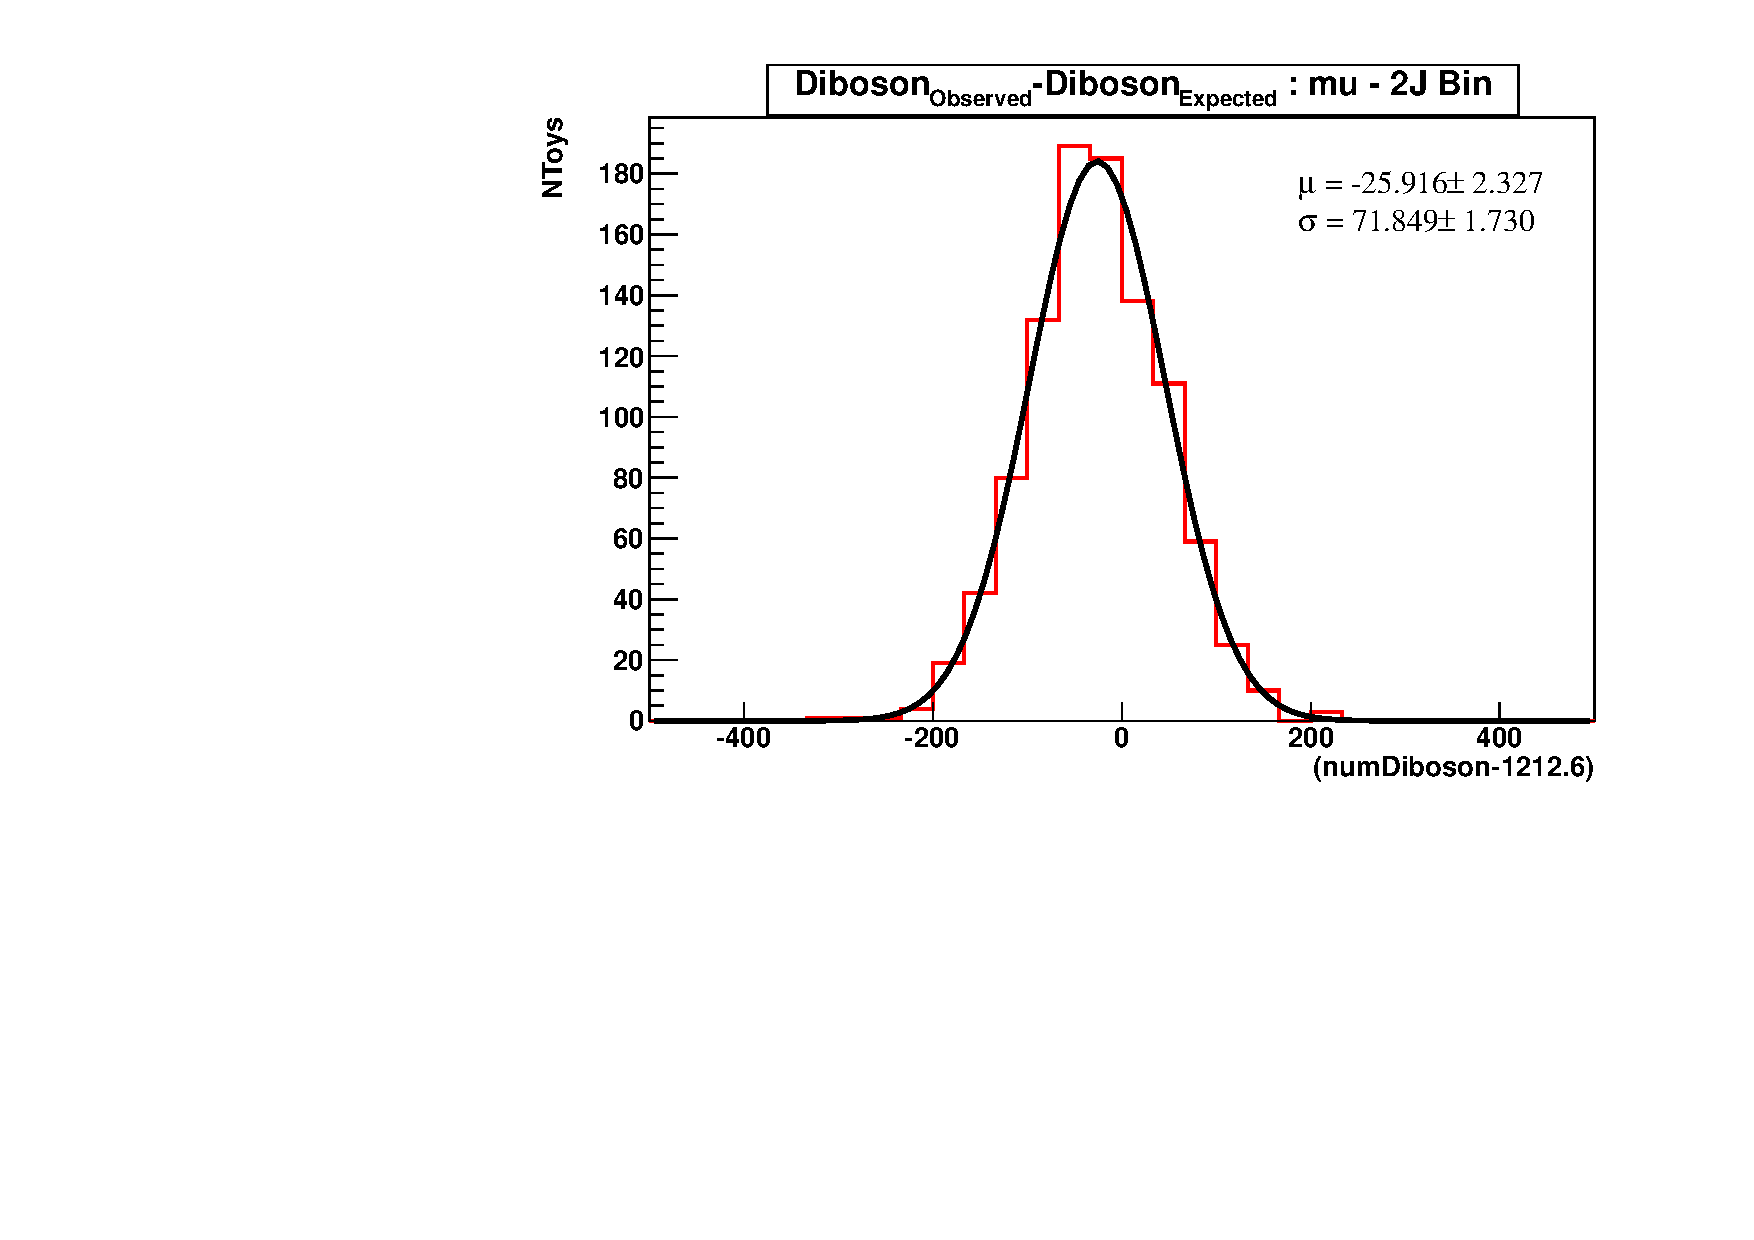
\includegraphics[width=0.48\textwidth]{figs/validation/DibosonYield_Validation_mu_2j.pdf}
\put(-0.80,0.0){(a)} 
\unitlength=0.33\linewidth
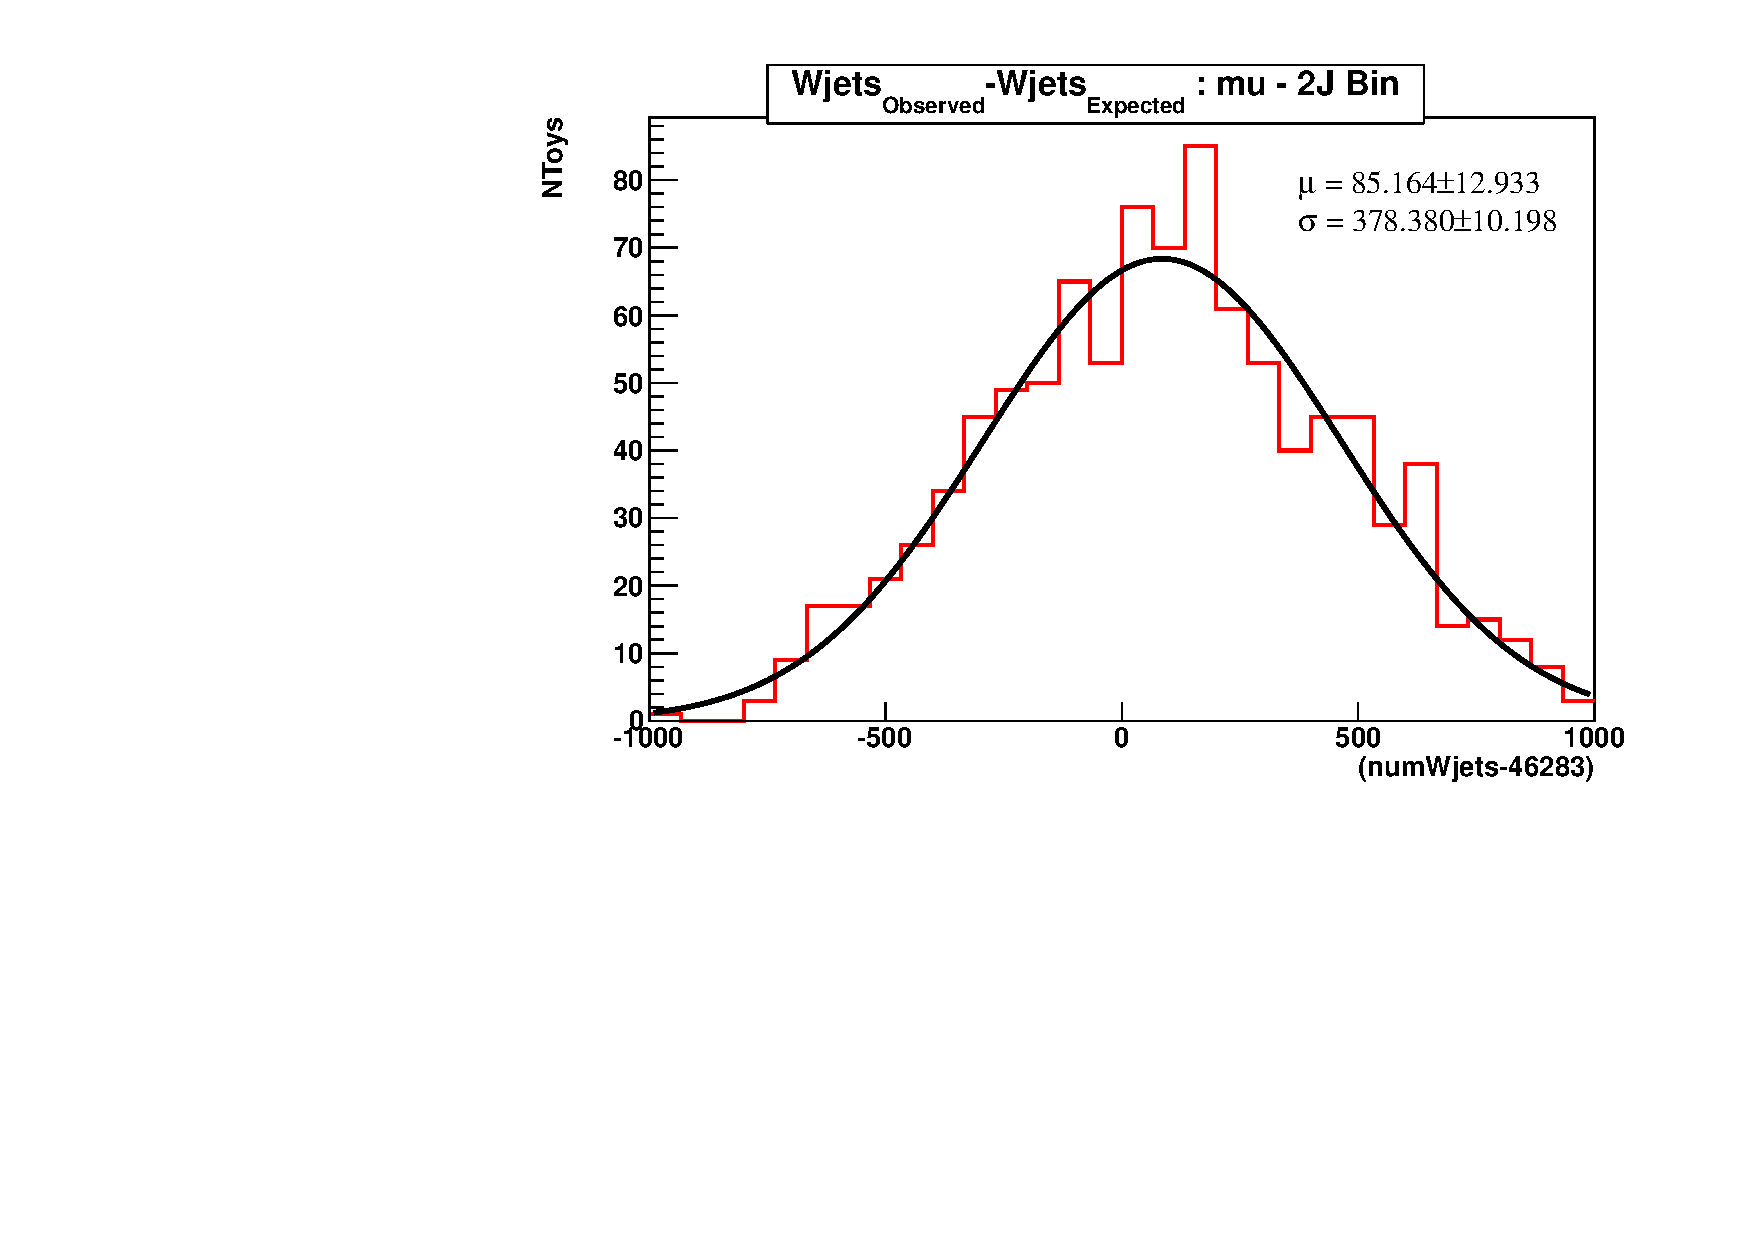
\includegraphics[width=0.48\textwidth]{figs/validation/WjetsYield_Validation_mu_2j.pdf}
\put(-0.80,0.0){(b)} \\
\unitlength=0.33\linewidth
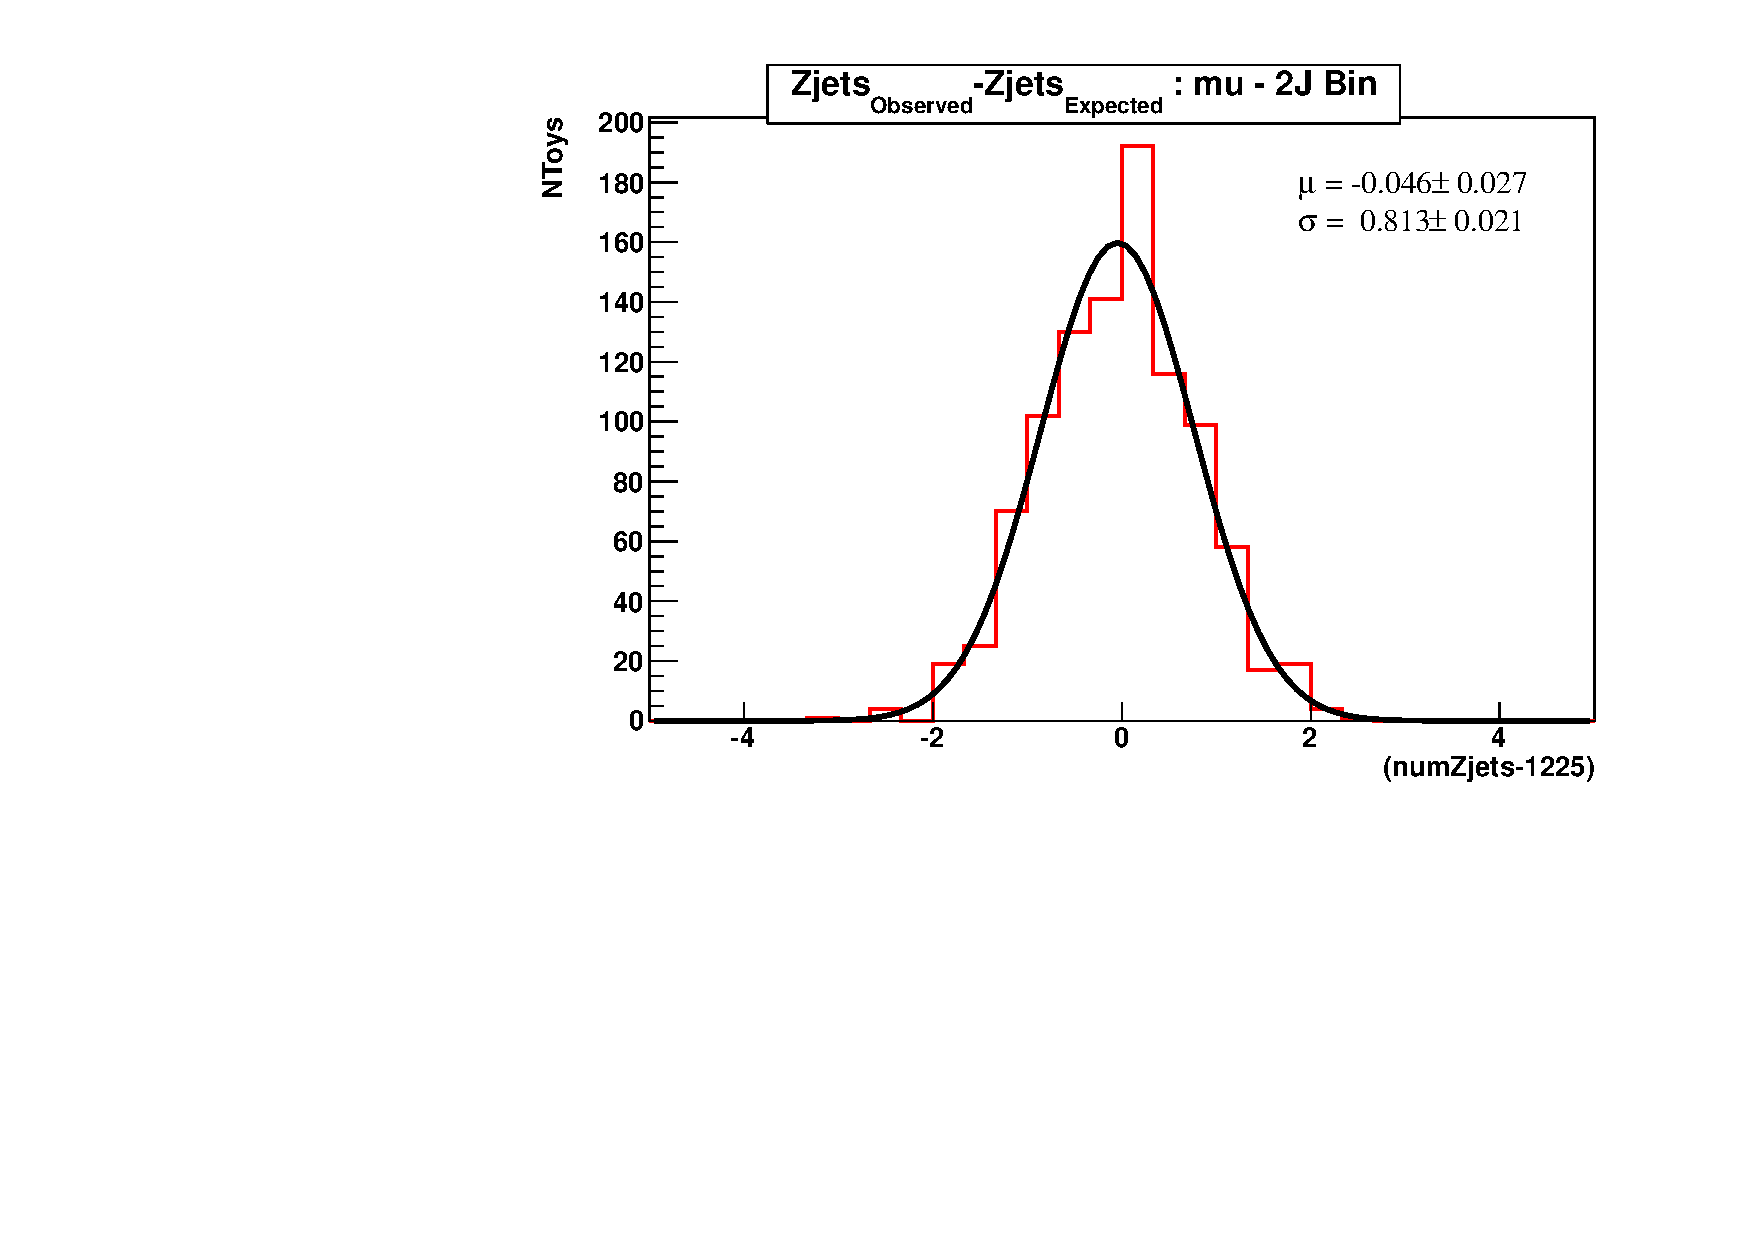
\includegraphics[width=0.48\textwidth]{figs/validation/ZjetsYield_Validation_mu_2j.pdf}
\put(-0.80,0.0){(c)} 
\unitlength=0.33\linewidth
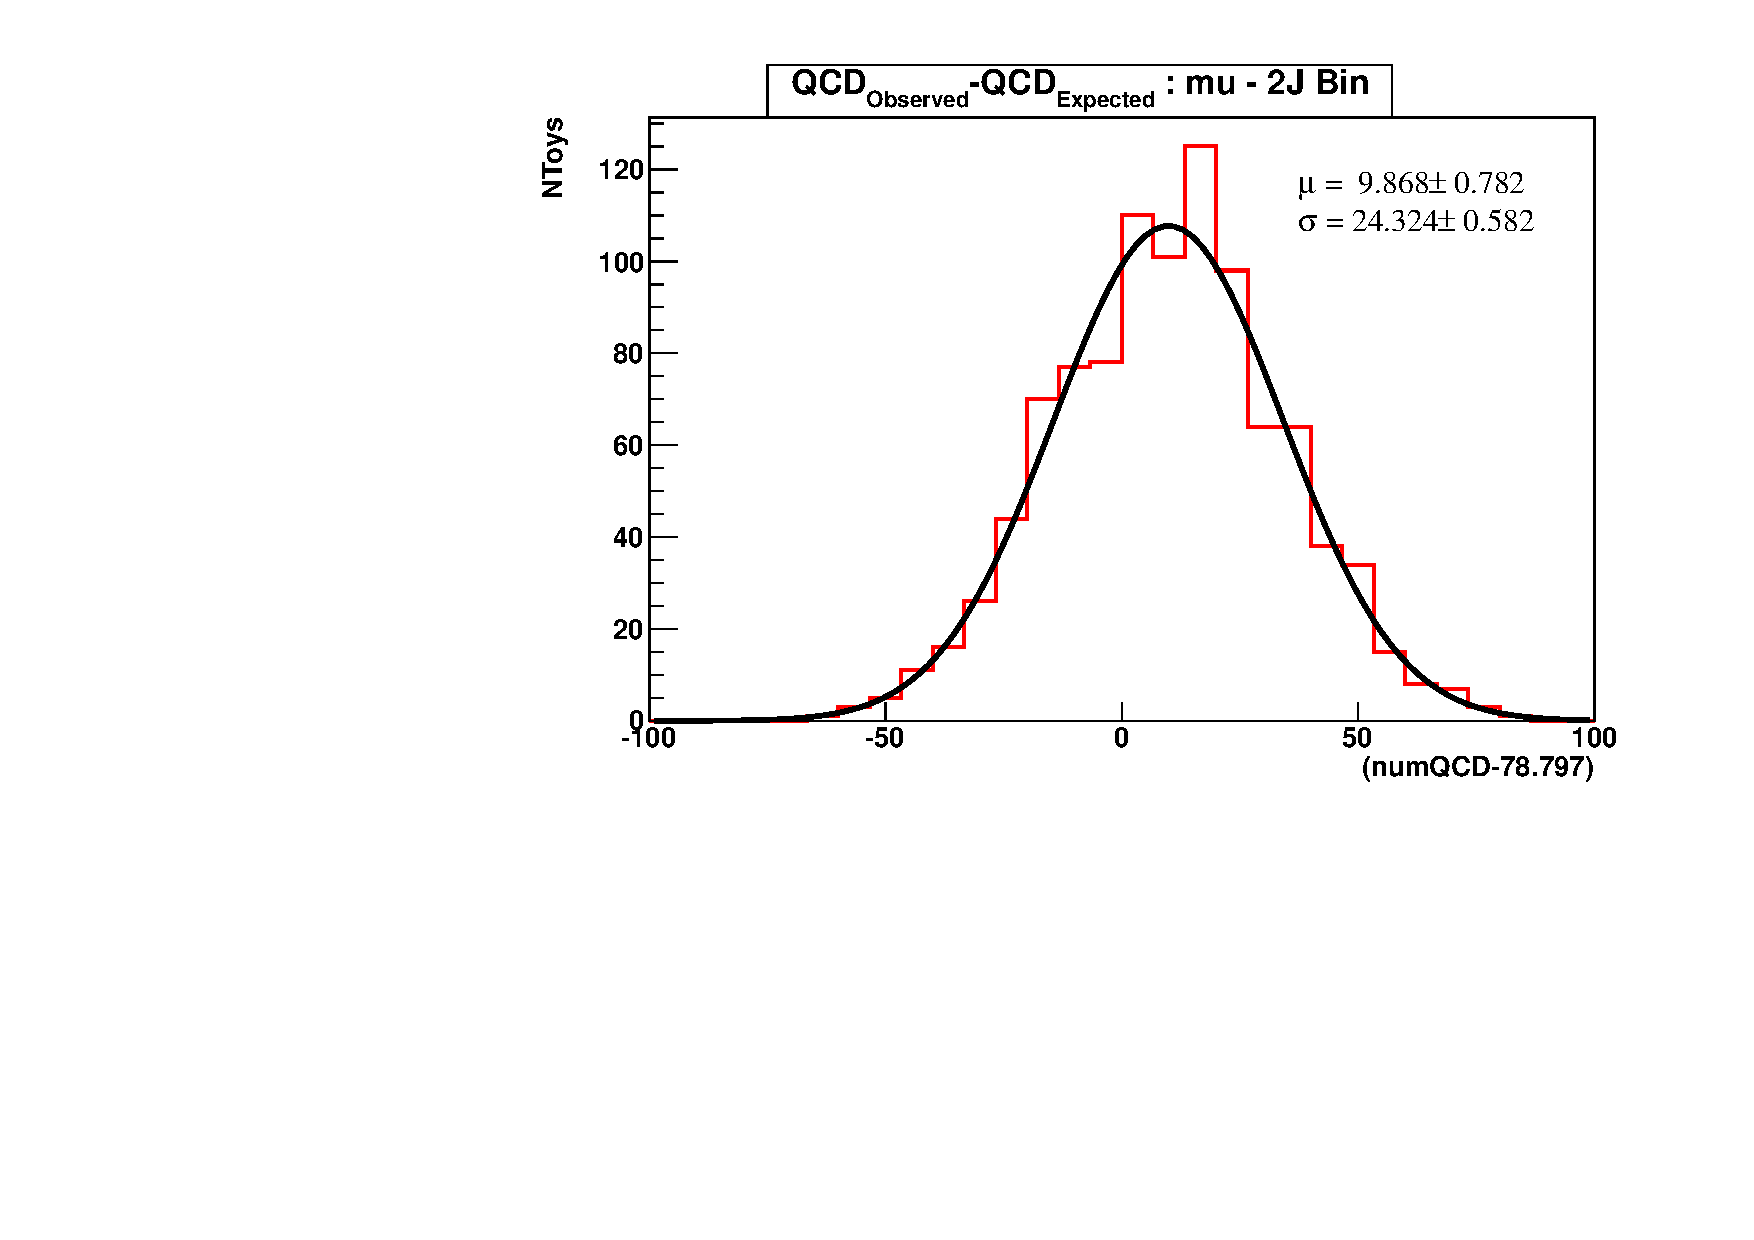
\includegraphics[width=0.48\textwidth]{figs/validation/QCDYield_Validation_mu_2j.pdf}
\put(-0.80,0.0){(d)} \\
\unitlength=0.33\linewidth
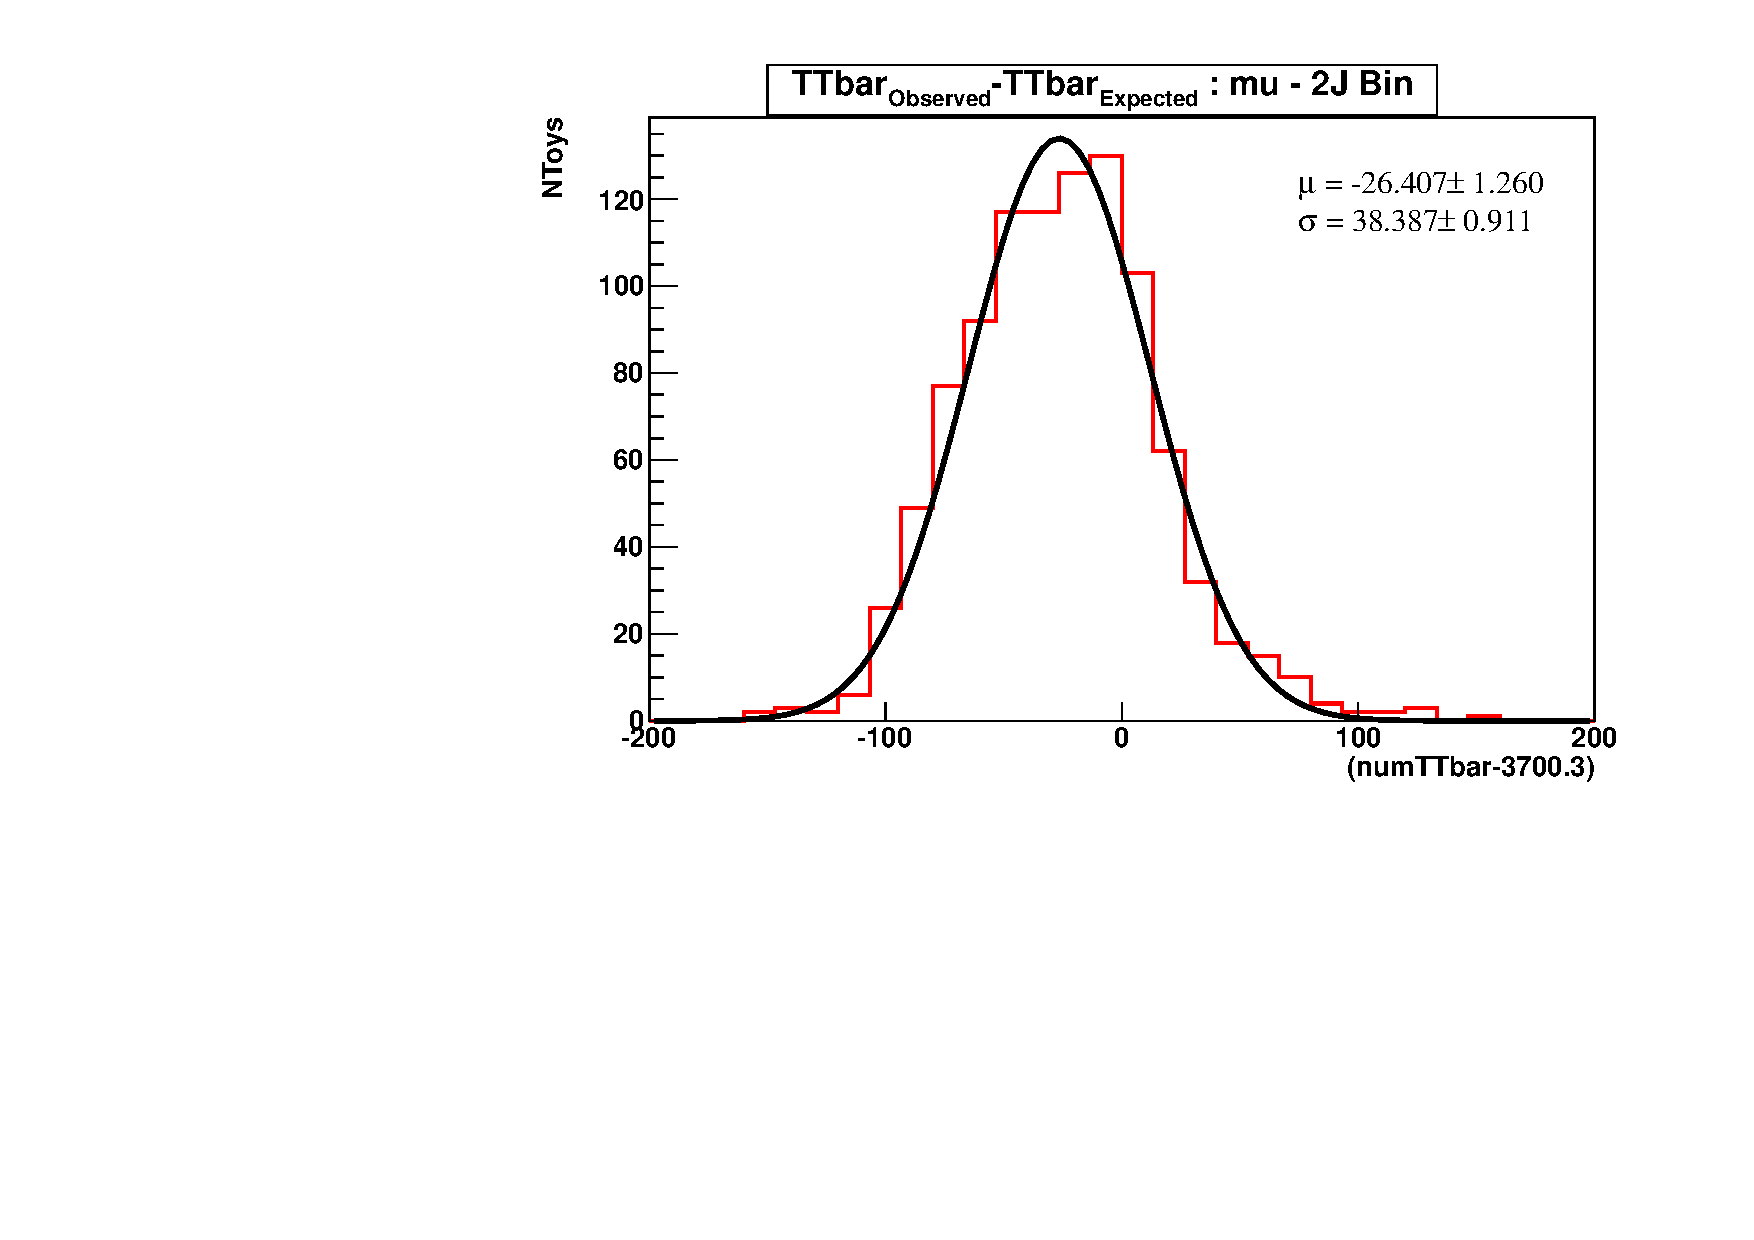
\includegraphics[width=0.48\textwidth]{figs/validation/TTbarYield_Validation_mu_2j.pdf}
\put(-0.80,0.0){(e)} 
\unitlength=0.33\linewidth
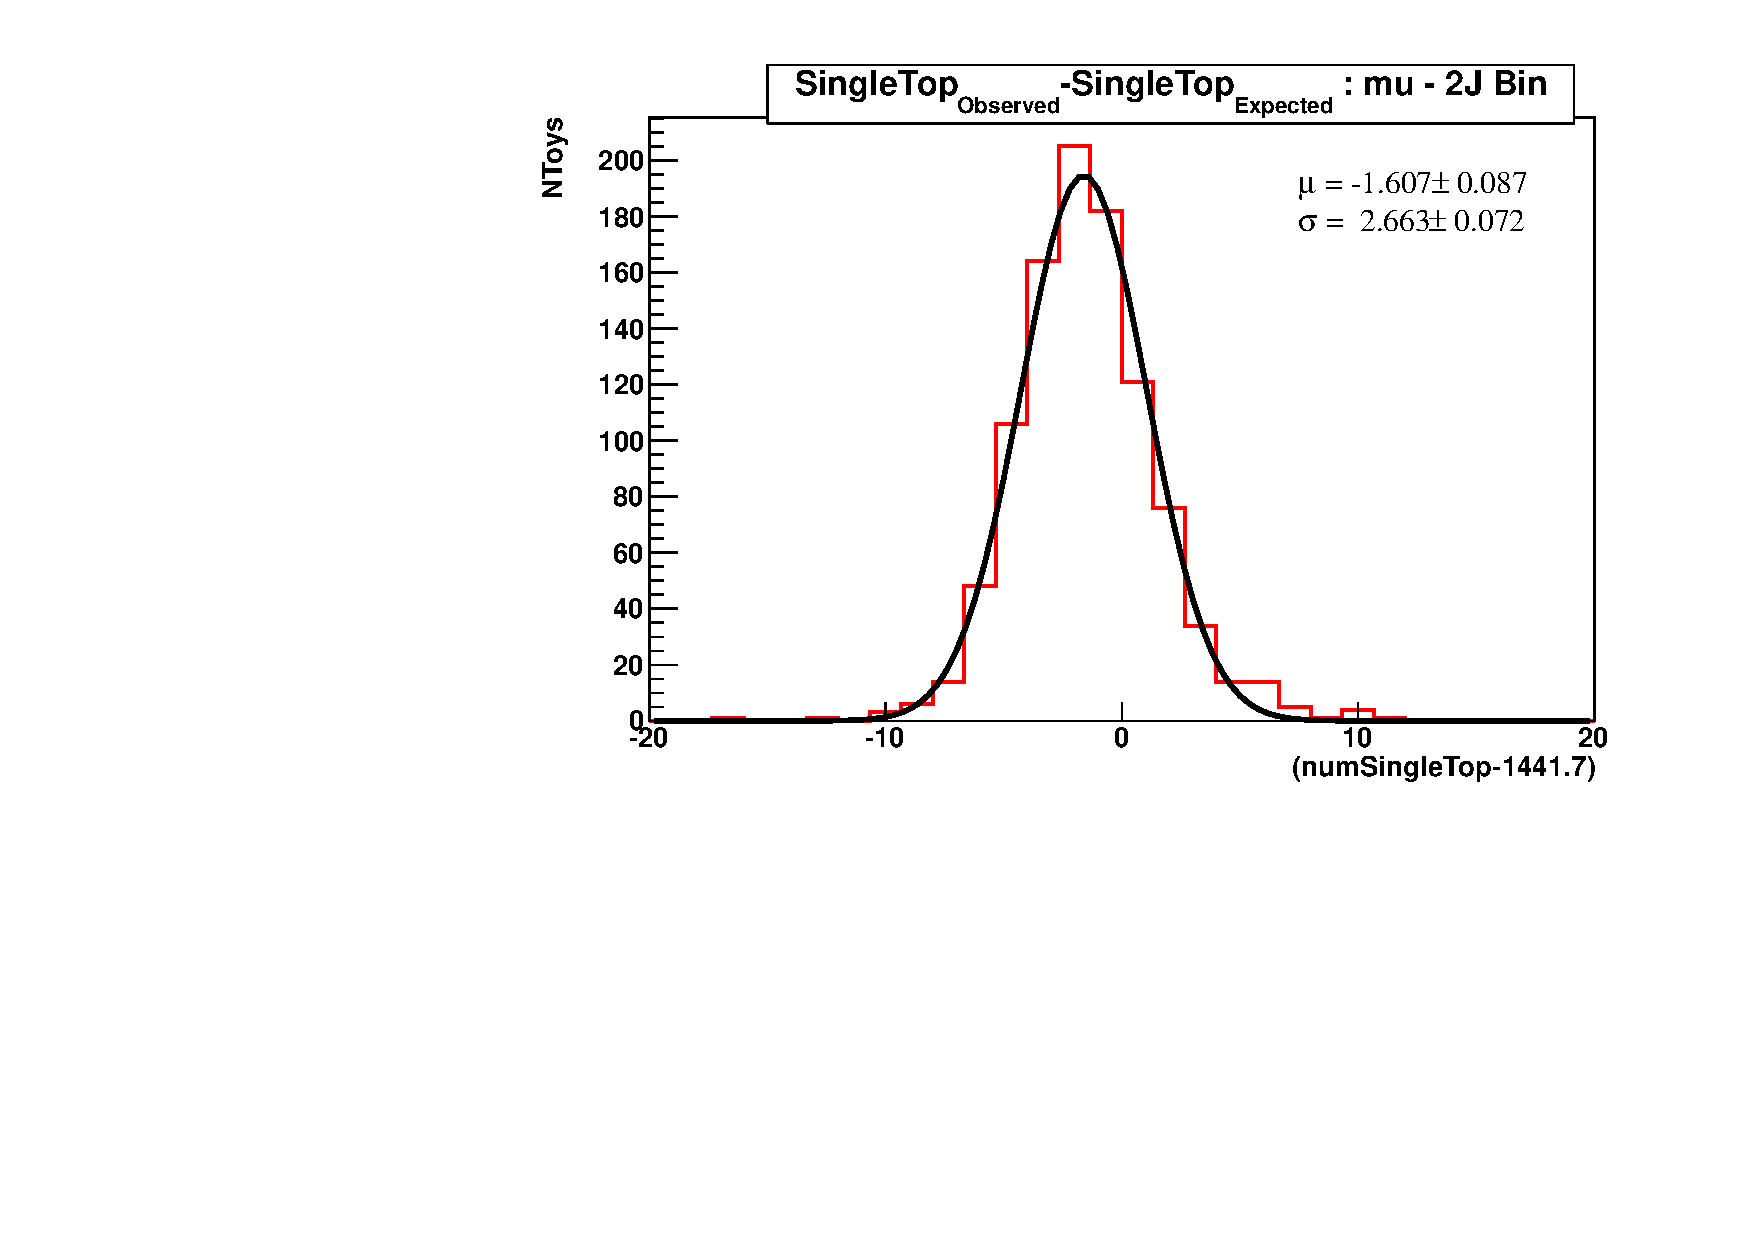
\includegraphics[width=0.48\textwidth]{figs/validation/SingleTopYield_Validation_mu_2j.pdf}
\put(-0.80,0.0){(f)} 
\caption{Fit validation in the 2-jet bin of the muon channel, using 1000 Toy MC datasets. Fitted-Expected yields for: (a) Diboson, (b) W+jets, (c) Z+jets, (d) QCD, (e) $t\bar{t}$, (f) SingleTop.} 
\label{fig:Validation_Yields_2j}}
\end{figure}
%%%%%%%
%%%%%%%
\begin{figure}[h!] {\centering
\unitlength=0.33\linewidth
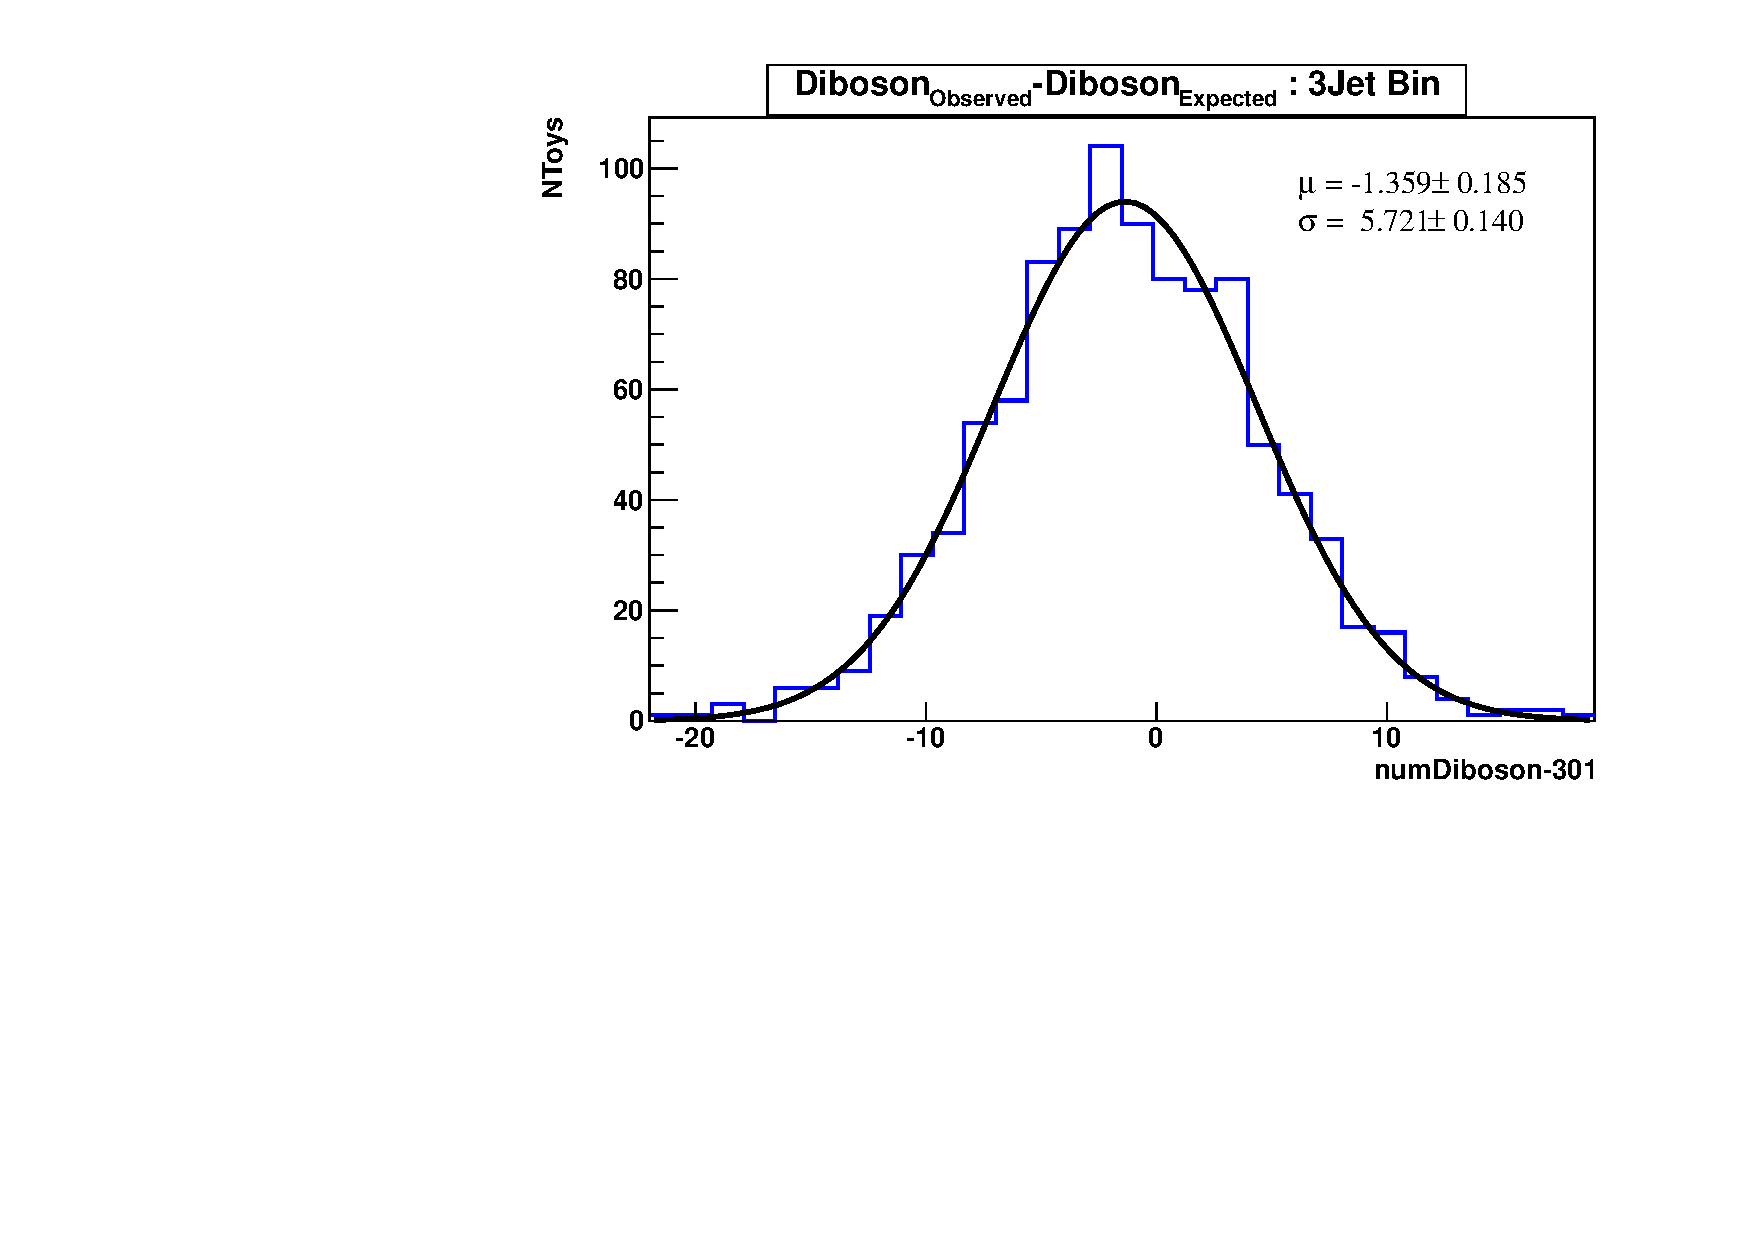
\includegraphics[width=0.48\textwidth]{figs/validation/DibosonYield_Validation_mu_3j.pdf}
\put(-0.80,0.0){(a)} 
\unitlength=0.33\linewidth
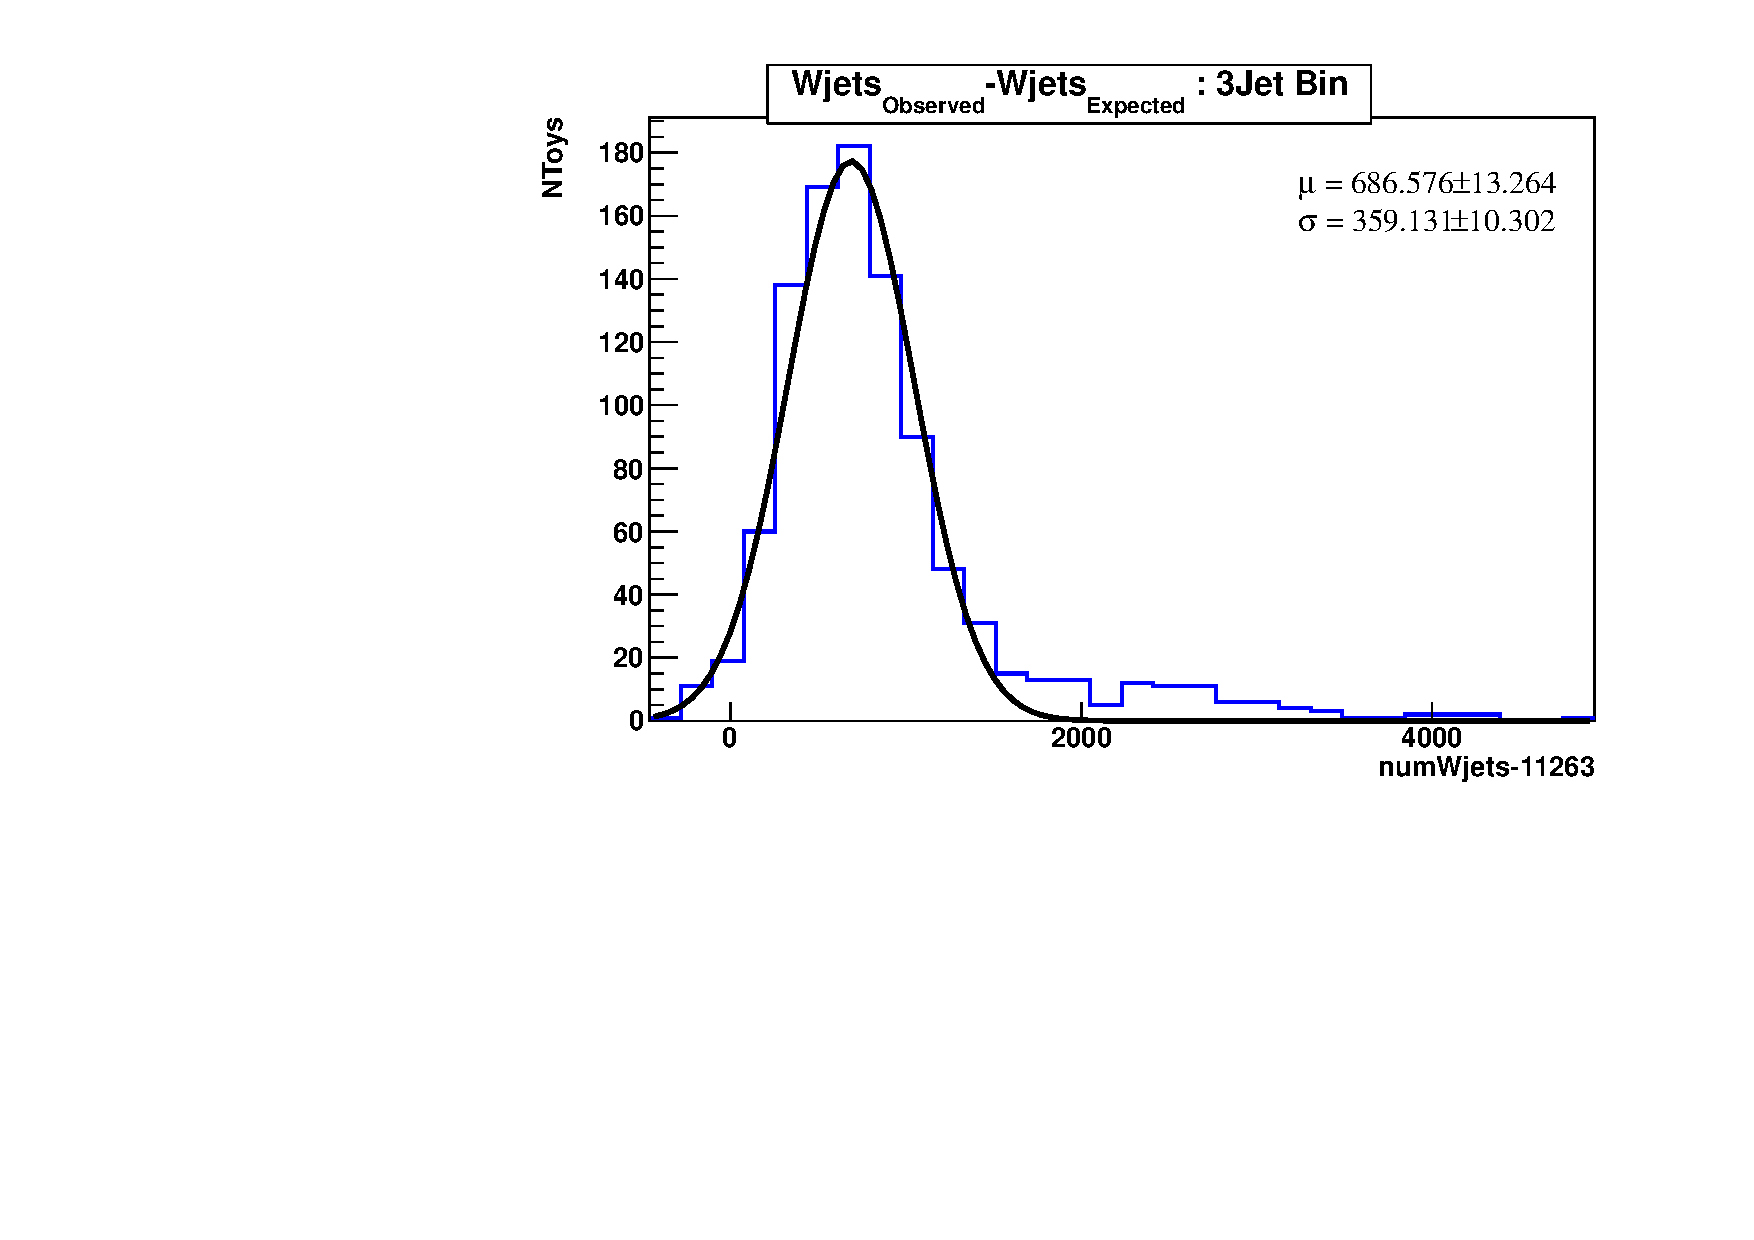
\includegraphics[width=0.48\textwidth]{figs/validation/WjetsYield_Validation_mu_3j.pdf}
\put(-0.80,0.0){(b)} \\
\unitlength=0.33\linewidth
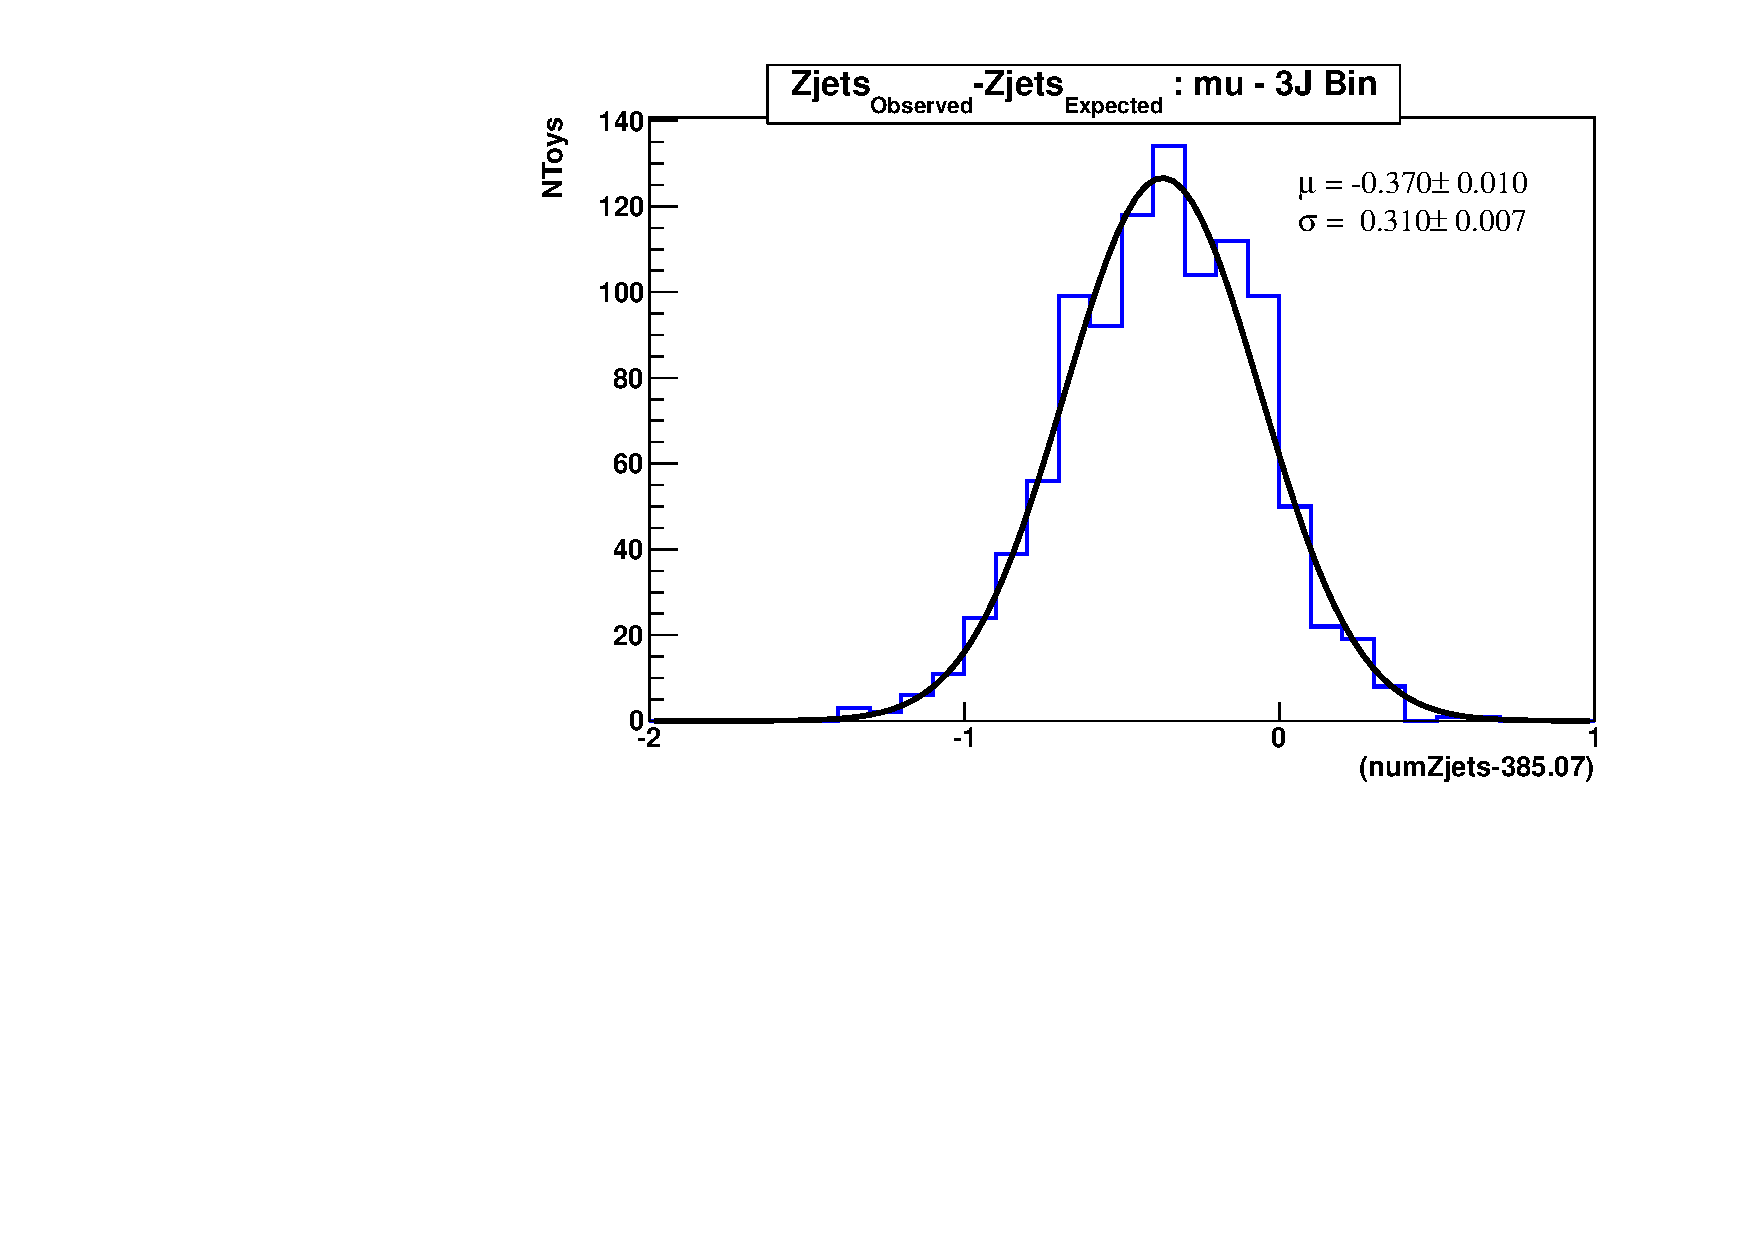
\includegraphics[width=0.48\textwidth]{figs/validation/ZjetsYield_Validation_mu_3j.pdf}
\put(-0.80,0.0){(c)} 
\unitlength=0.33\linewidth
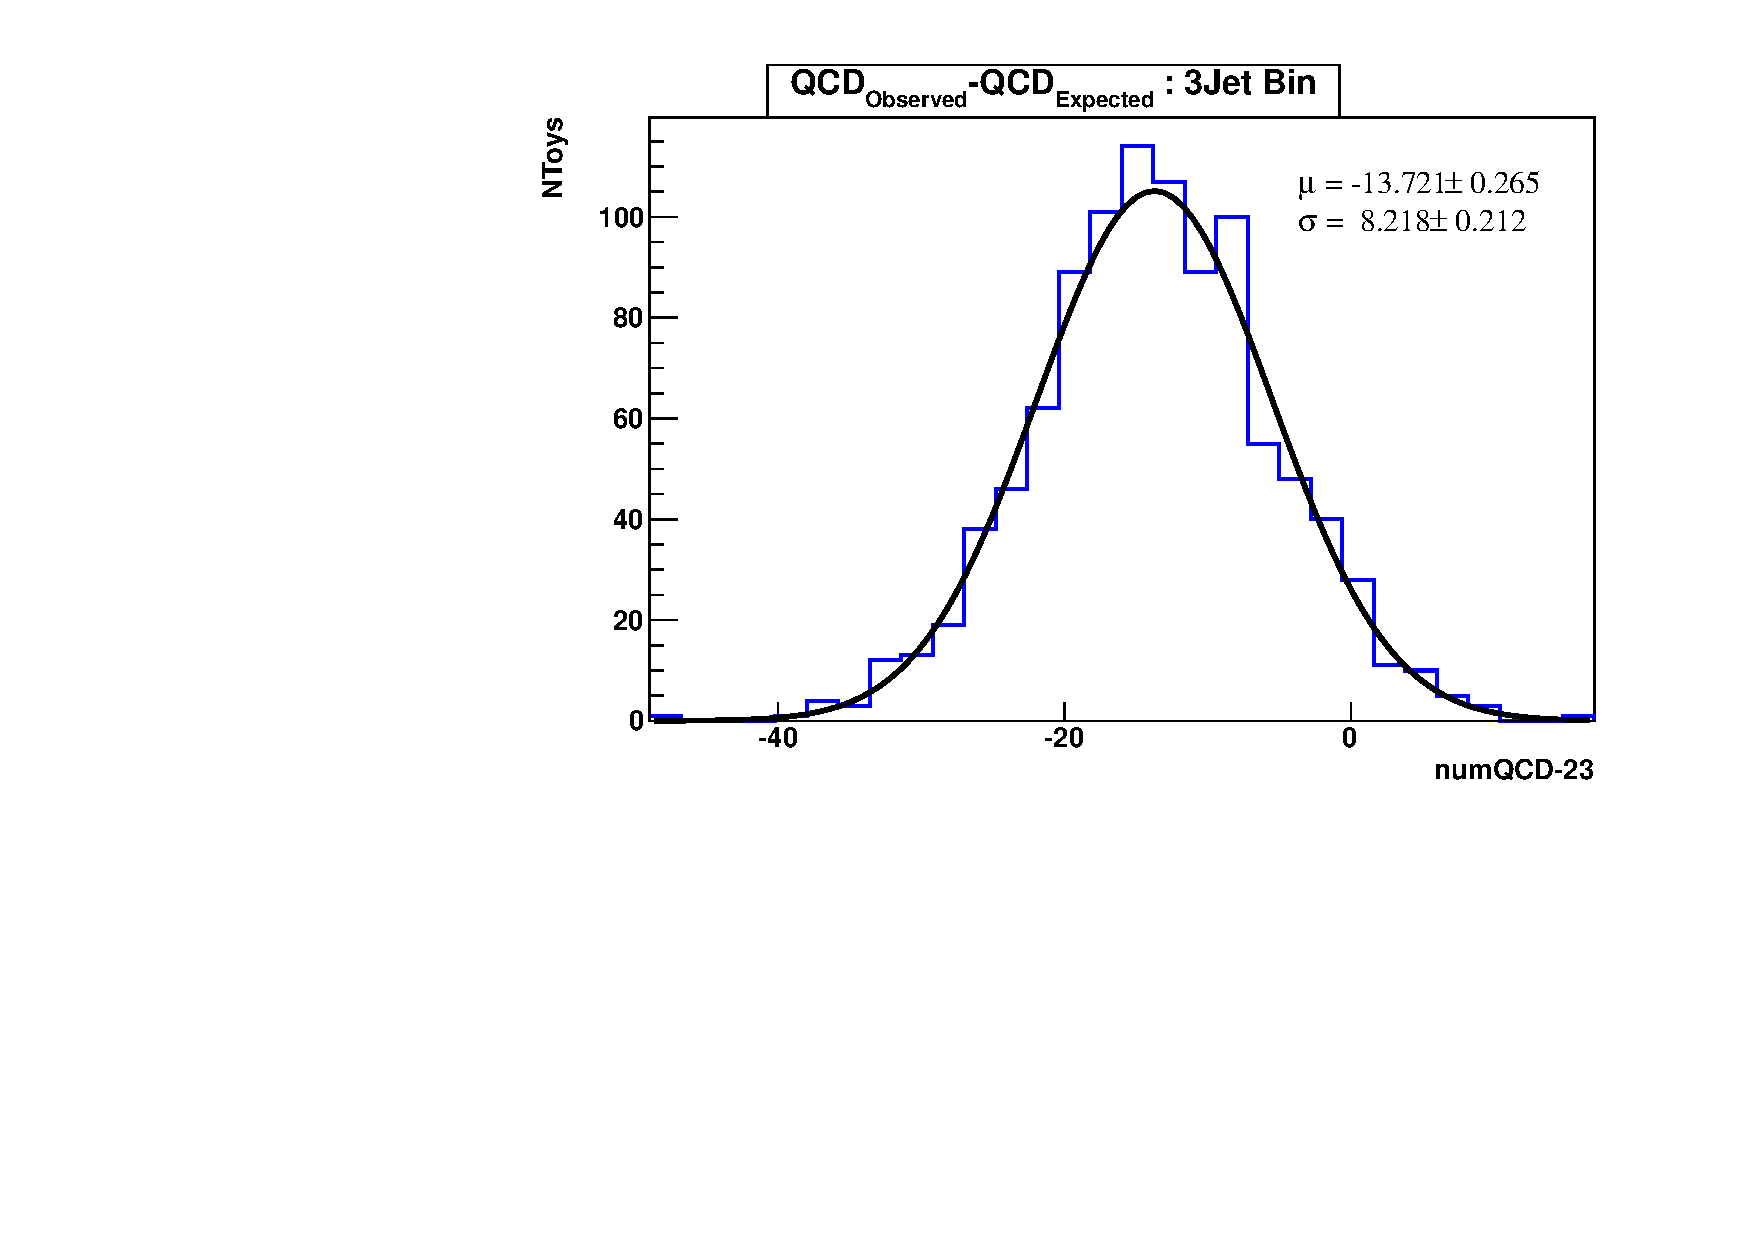
\includegraphics[width=0.48\textwidth]{figs/validation/QCDYield_Validation_mu_3j.pdf}
\put(-0.80,0.0){(d)} \\
\unitlength=0.33\linewidth
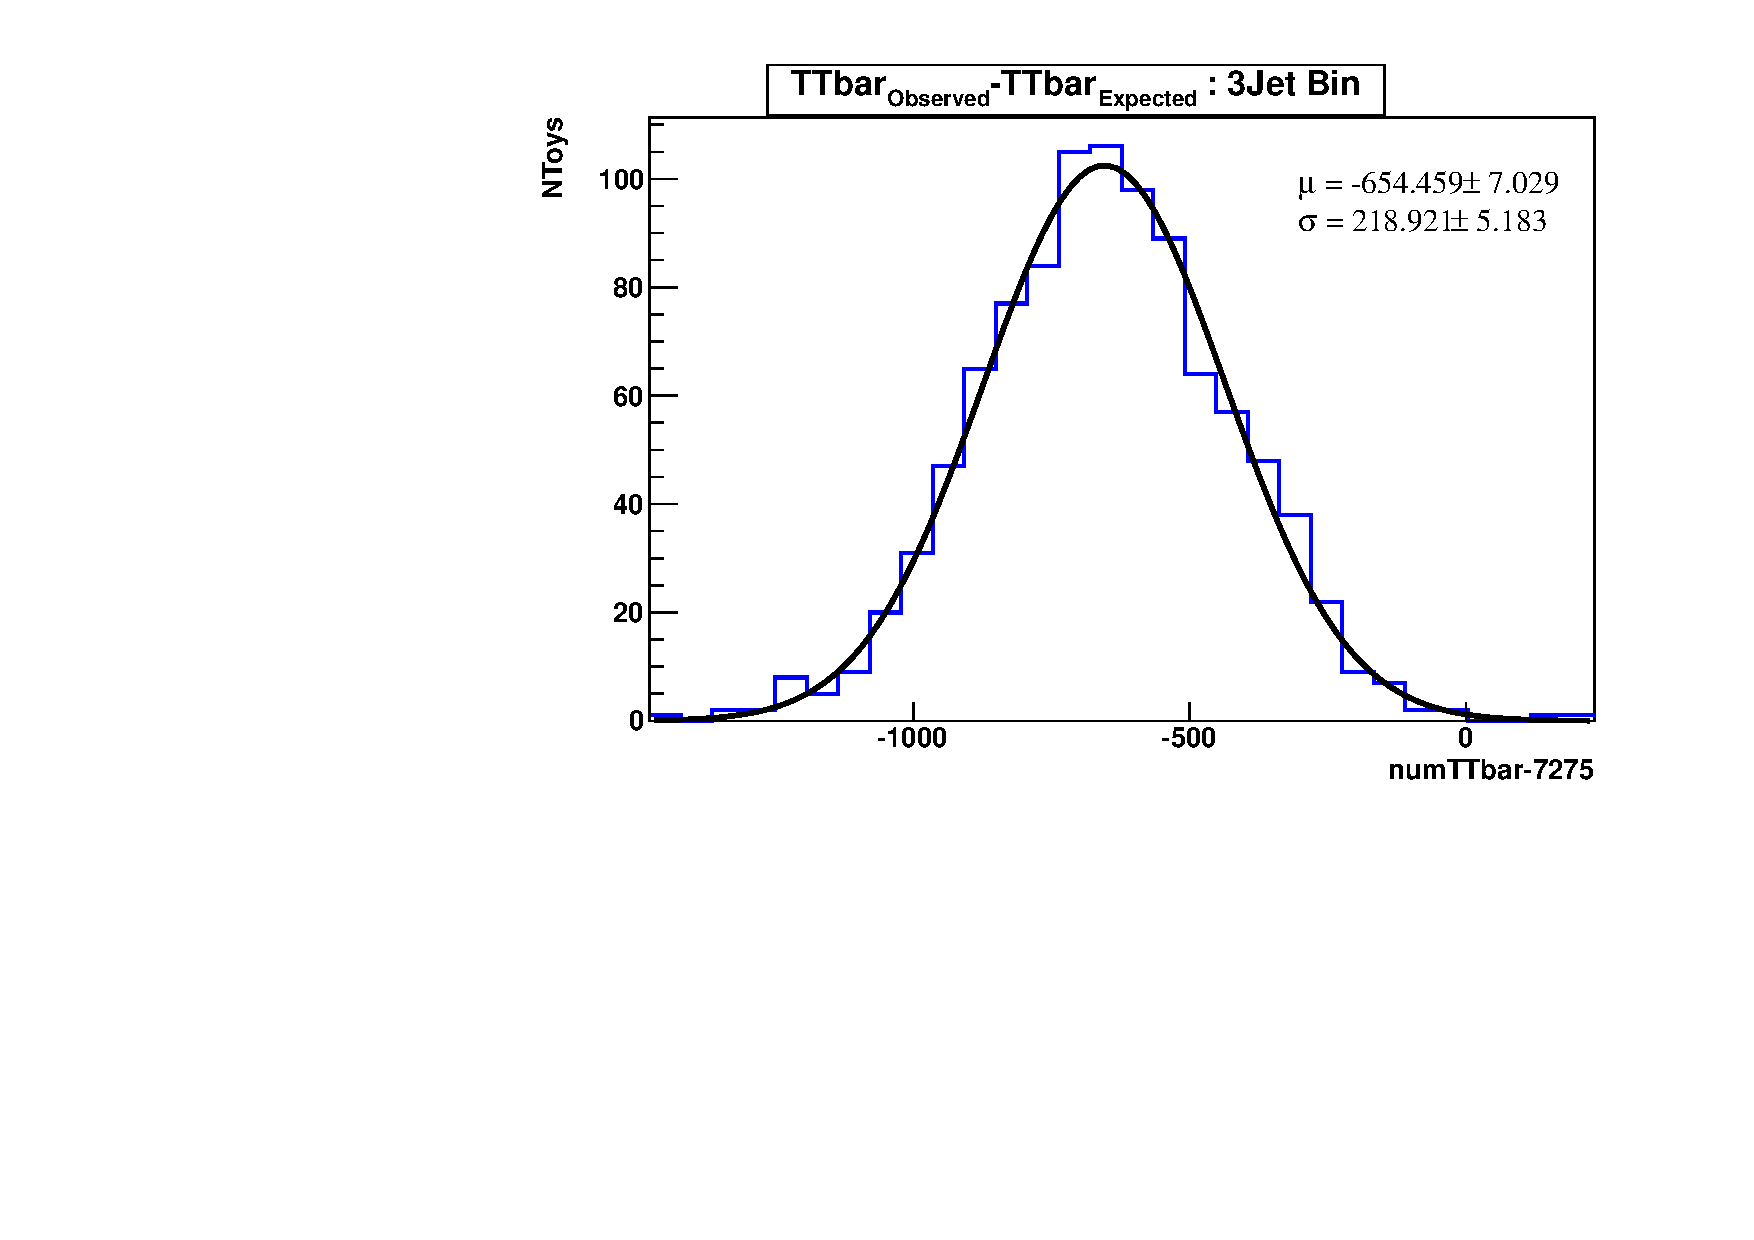
\includegraphics[width=0.48\textwidth]{figs/validation/TTbarYield_Validation_mu_3j.pdf}
\put(-0.80,0.0){(e)} 
\unitlength=0.33\linewidth
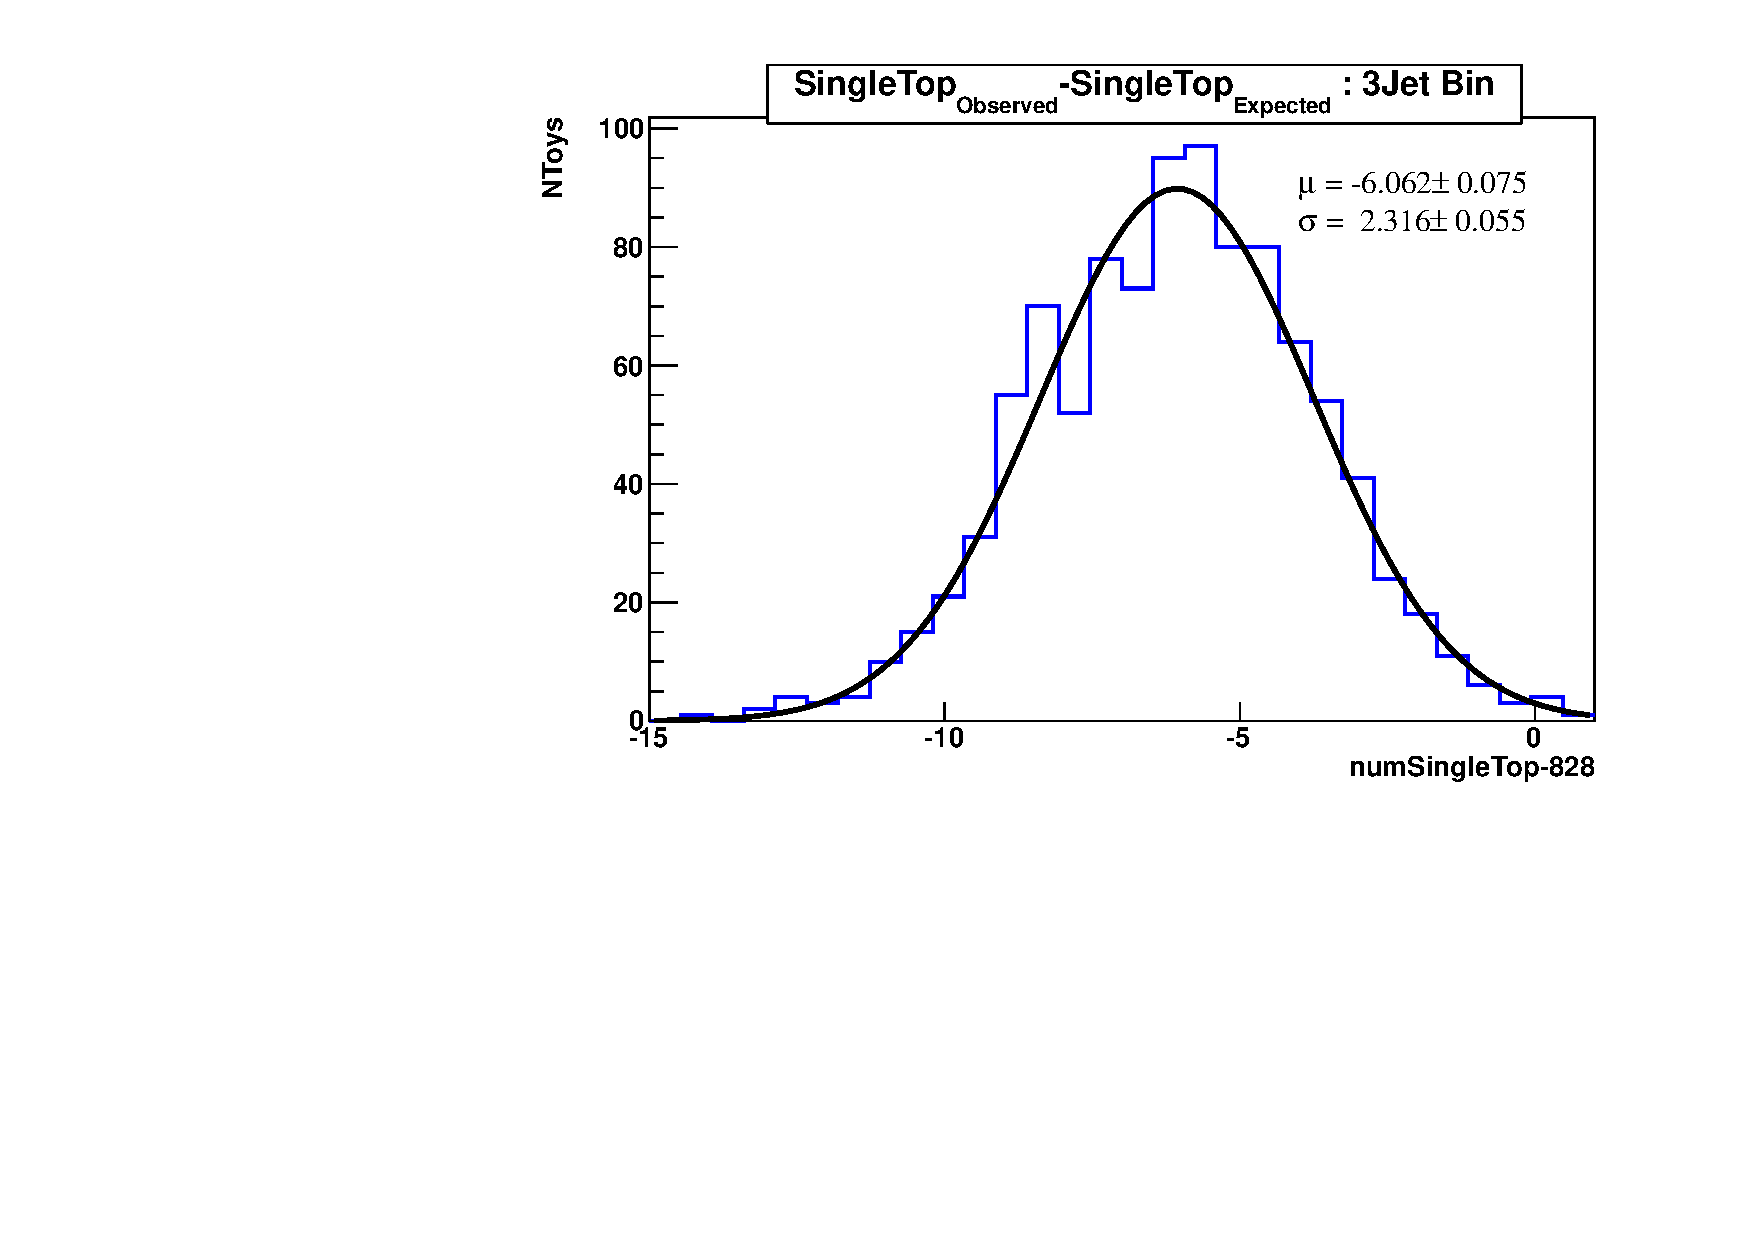
\includegraphics[width=0.48\textwidth]{figs/validation/SingleTopYield_Validation_mu_3j.pdf}
\put(-0.80,0.0){(f)} 
\caption{Fit validation in the 3-jet bin of the muon channel, using 1000 Toy MC datasets. Fitted-Expected yields for: (a) Diboson, (b) W+jets, (c) Z+jets, (d) QCD, (e) $t\bar{t}$, (f) SingleTop.} 
\label{fig:Validation_Yields_3j}}
\end{figure}
%%%%%%%
%%%%%%%
\begin{figure}[h!] {\centering
\unitlength=0.33\linewidth
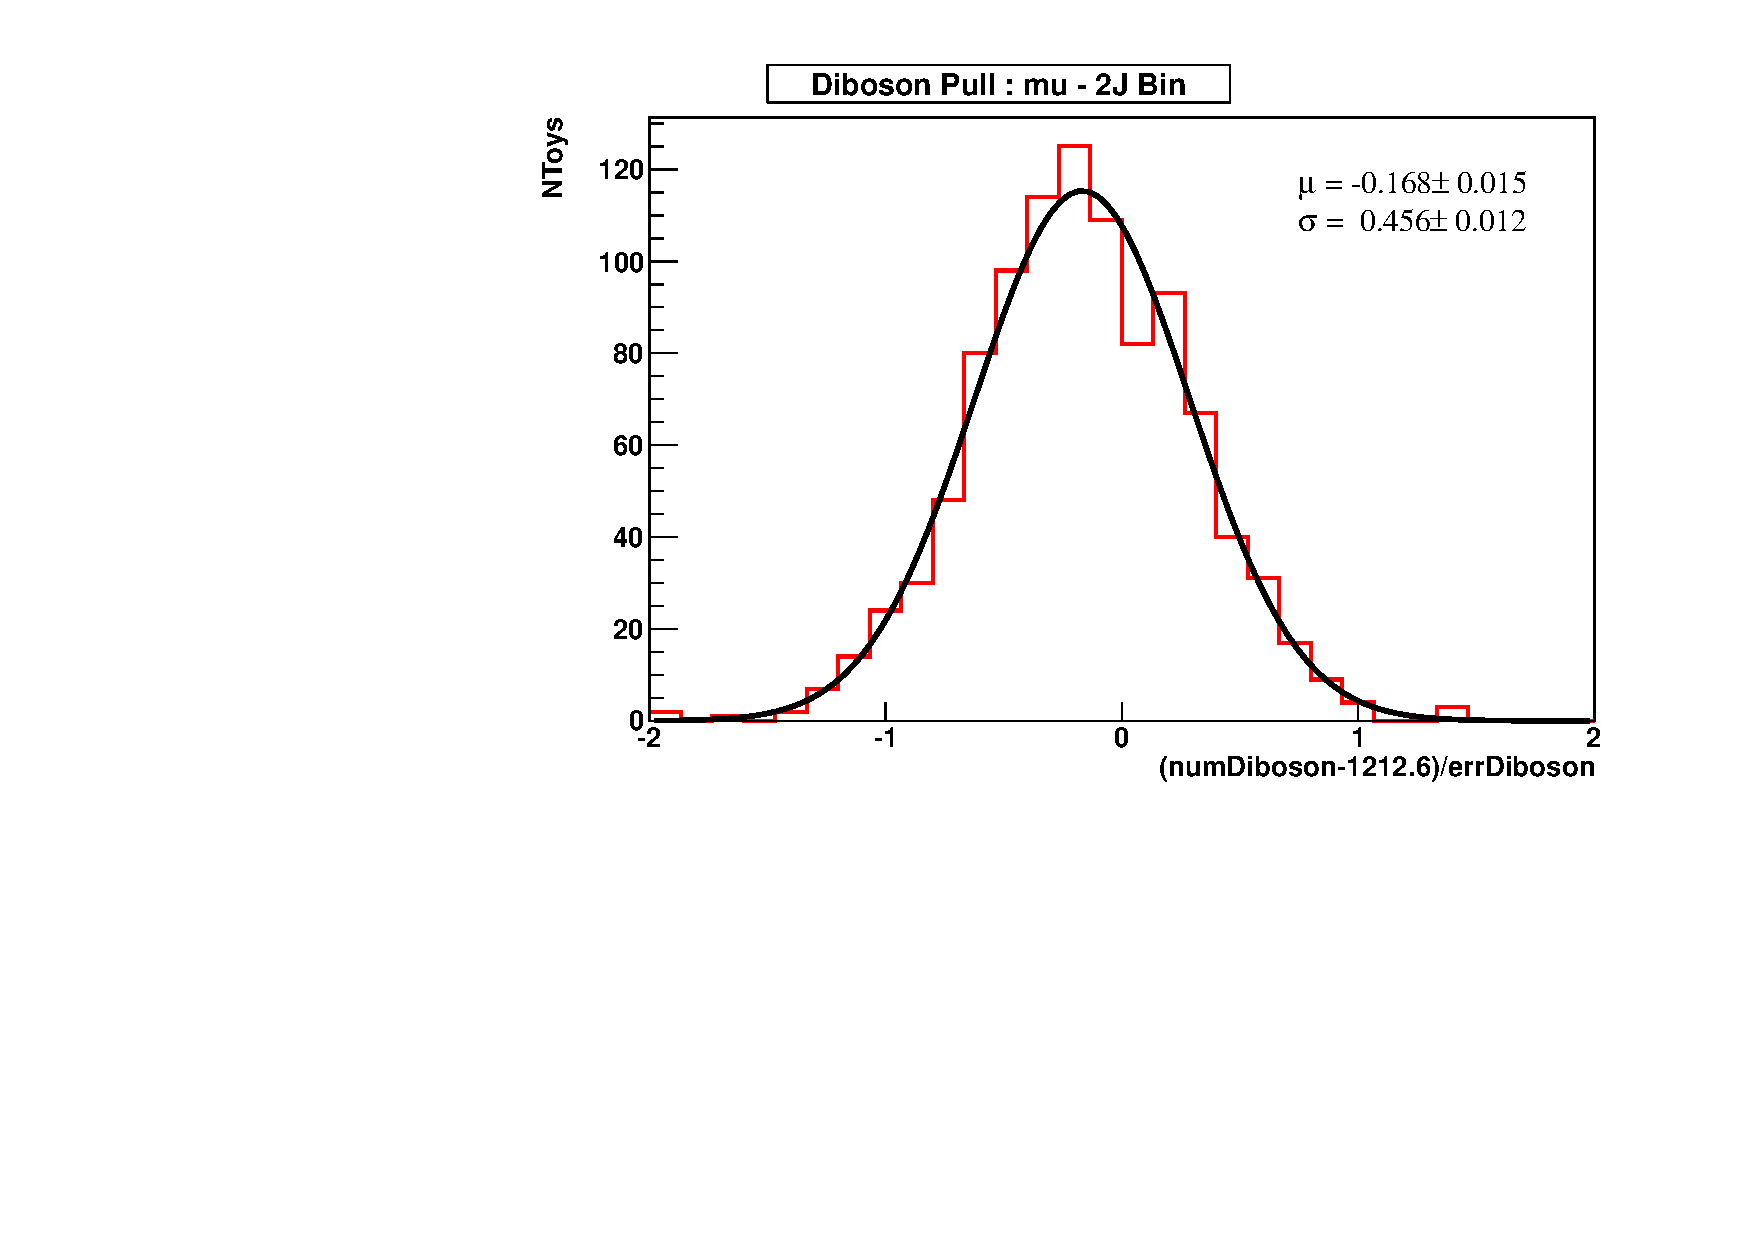
\includegraphics[width=0.48\textwidth]{figs/validation/DibosonPull_Validation_mu_2j.pdf}
\put(-0.80,0.0){(a)} 
\unitlength=0.33\linewidth
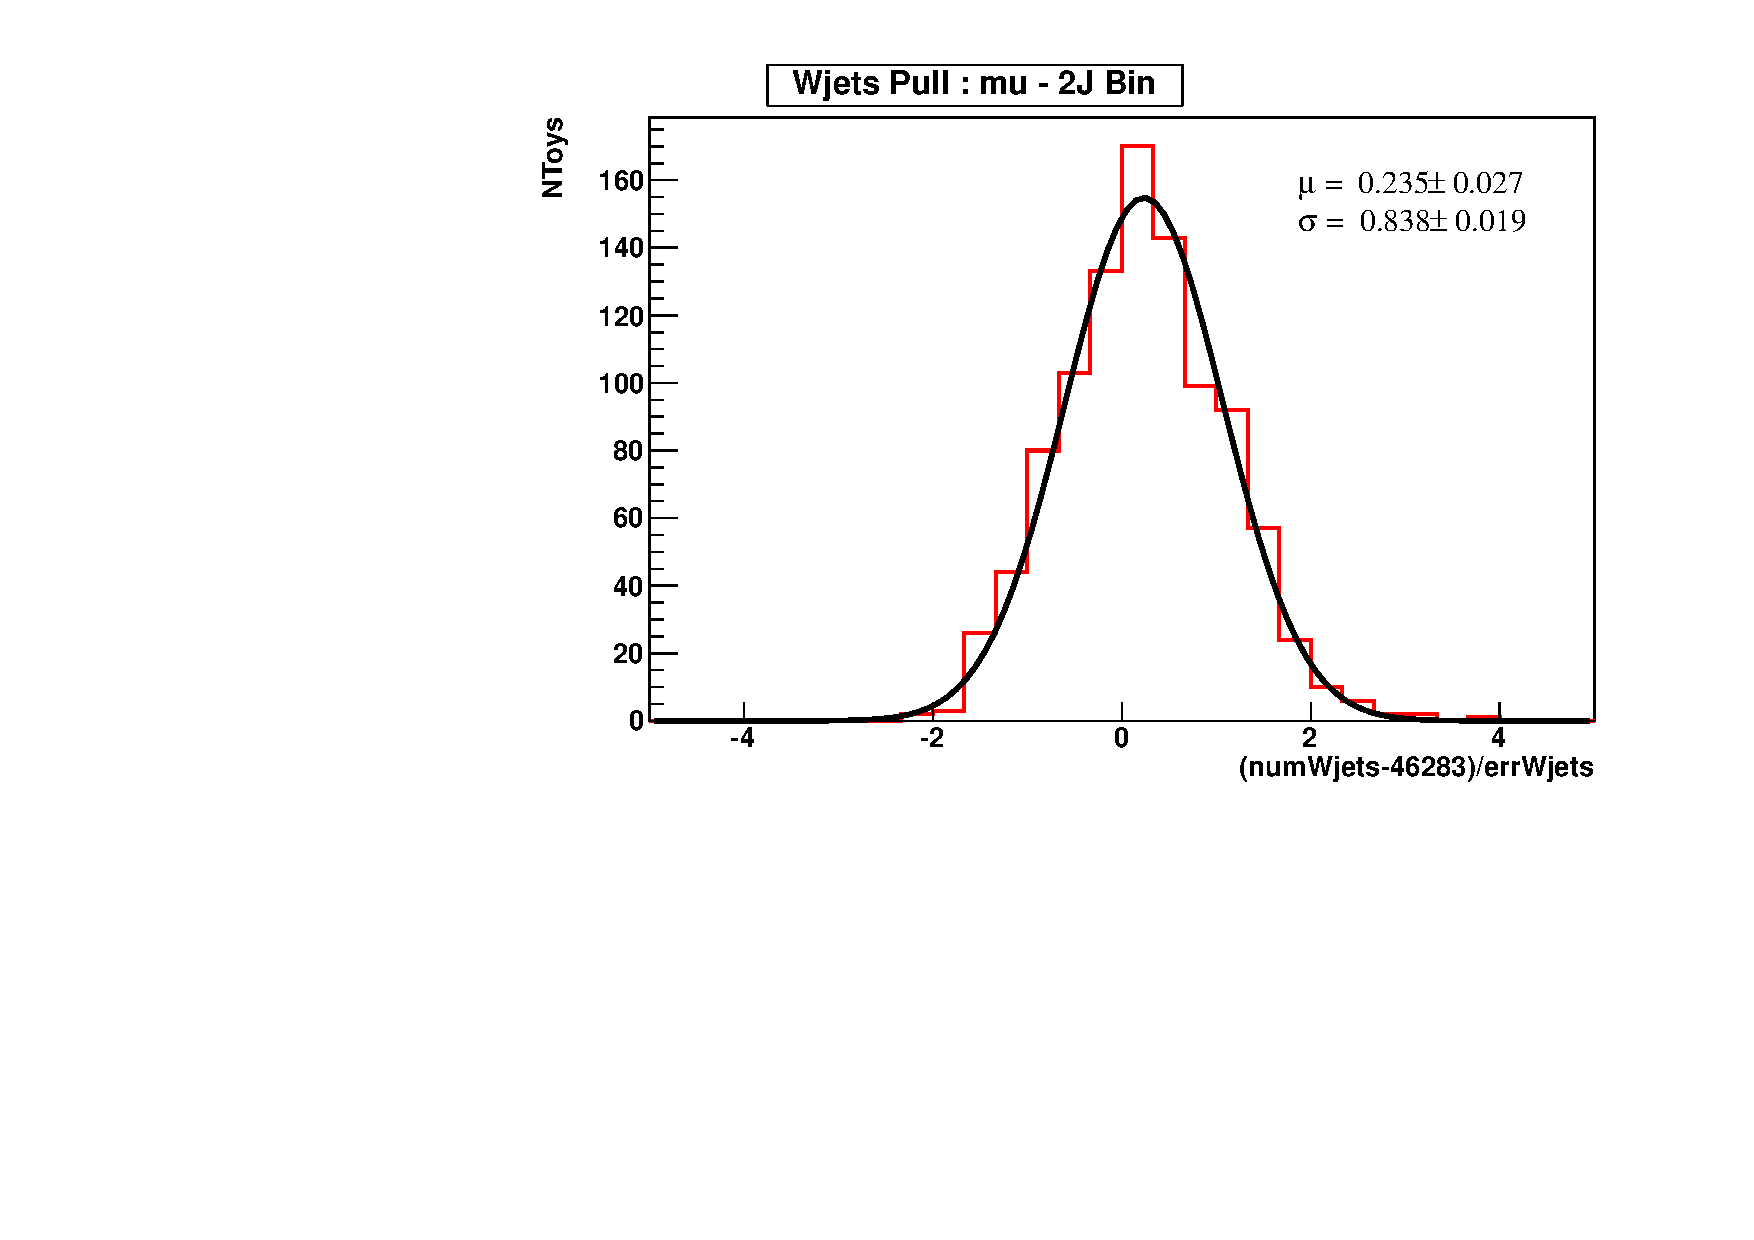
\includegraphics[width=0.48\textwidth]{figs/validation/WjetsPull_Validation_mu_2j.pdf}
\put(-0.80,0.0){(b)} \\
\unitlength=0.33\linewidth
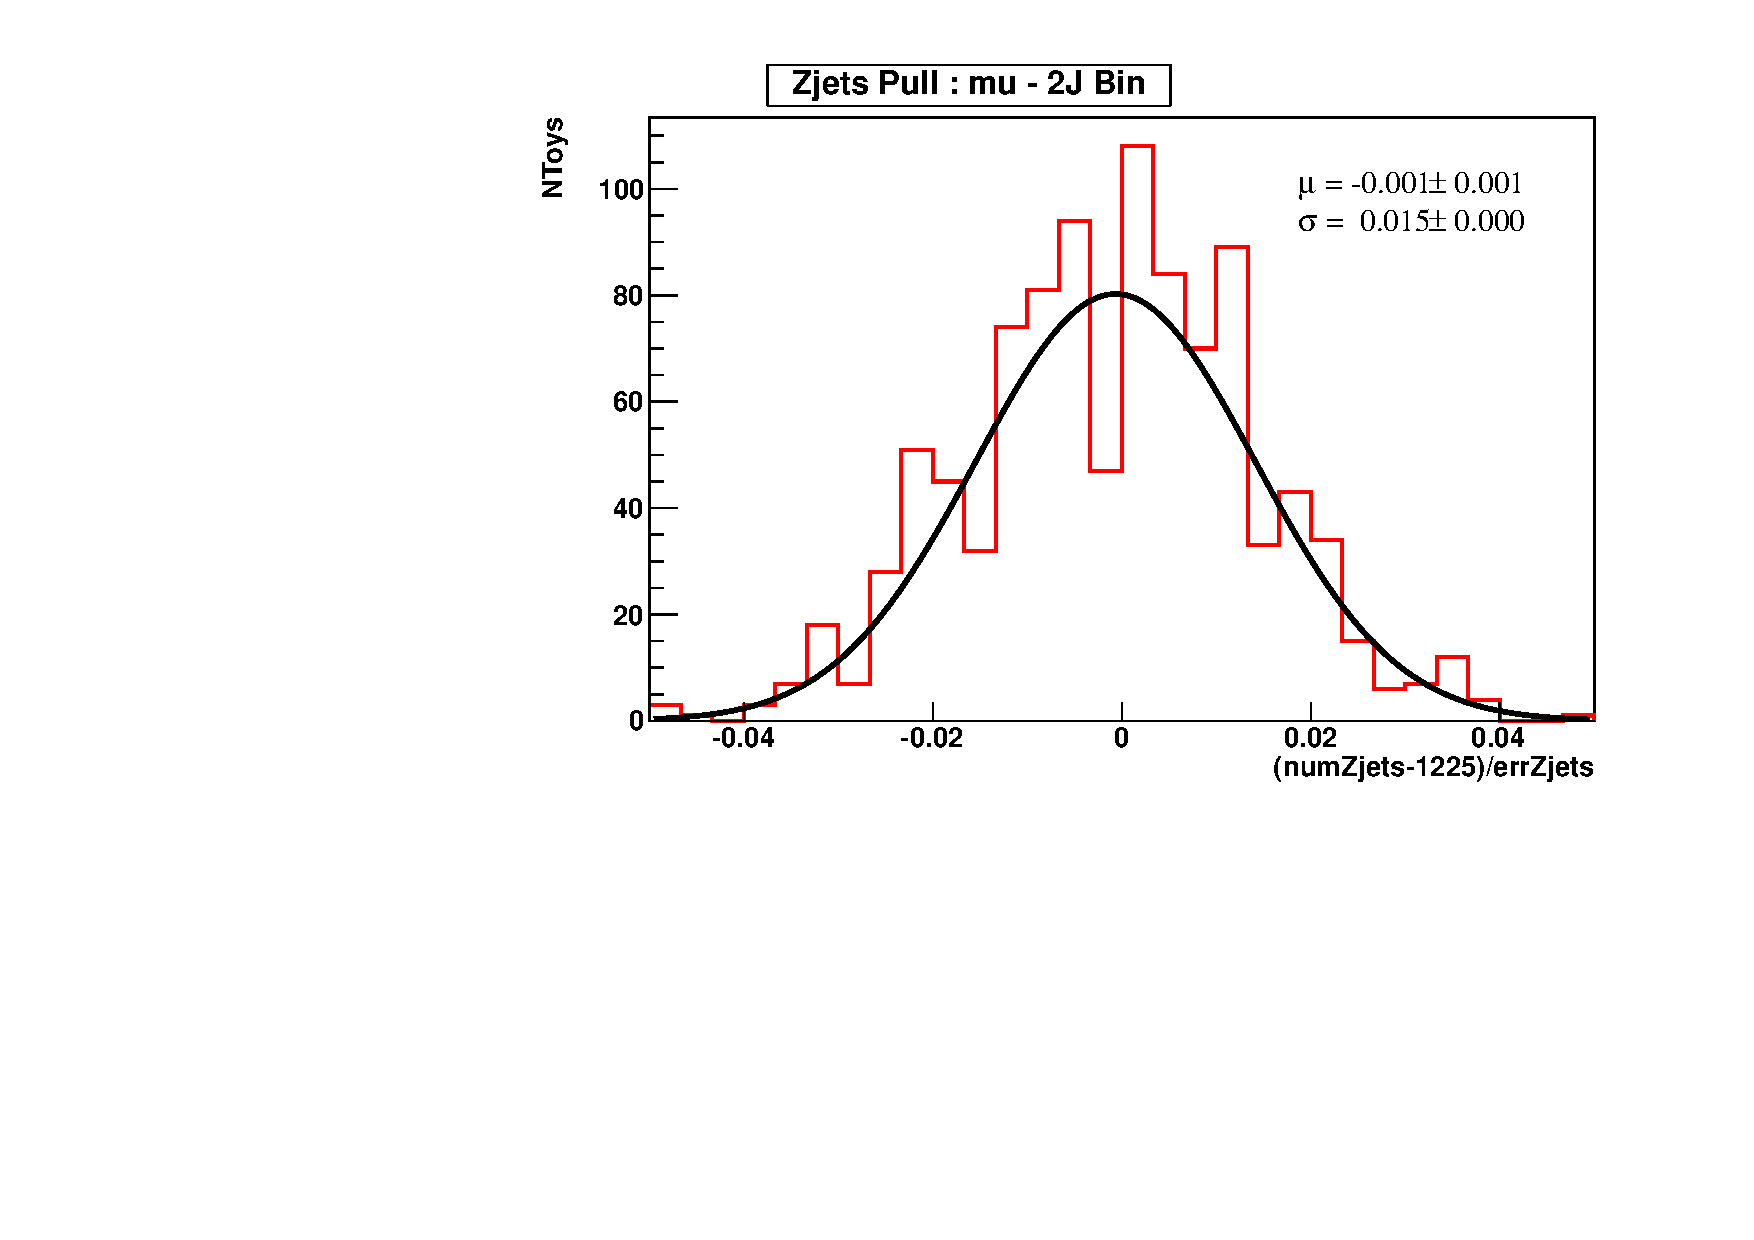
\includegraphics[width=0.48\textwidth]{figs/validation/ZjetsPull_Validation_mu_2j.pdf}
\put(-0.80,0.0){(c)} 
\unitlength=0.33\linewidth
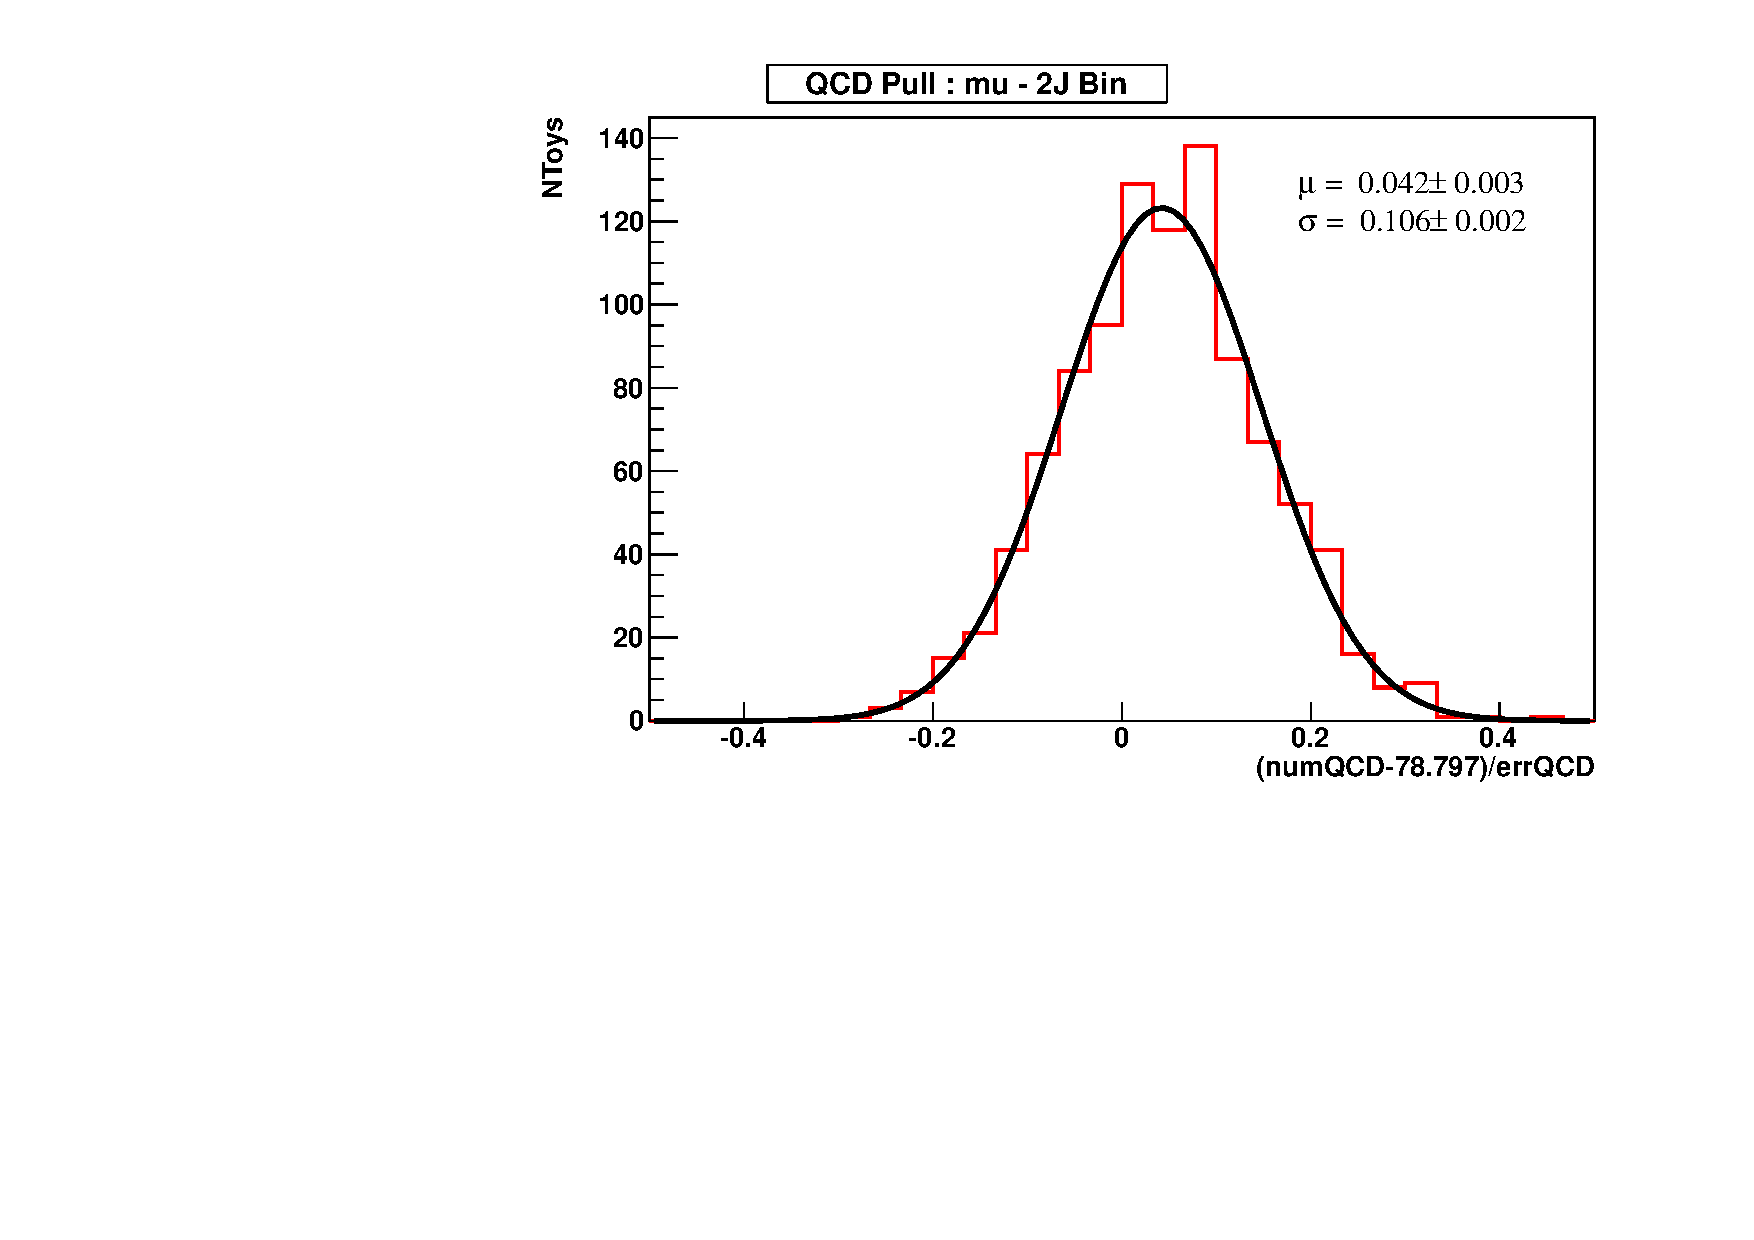
\includegraphics[width=0.48\textwidth]{figs/validation/QCDPull_Validation_mu_2j.pdf}
\put(-0.80,0.0){(d)} \\
\unitlength=0.33\linewidth
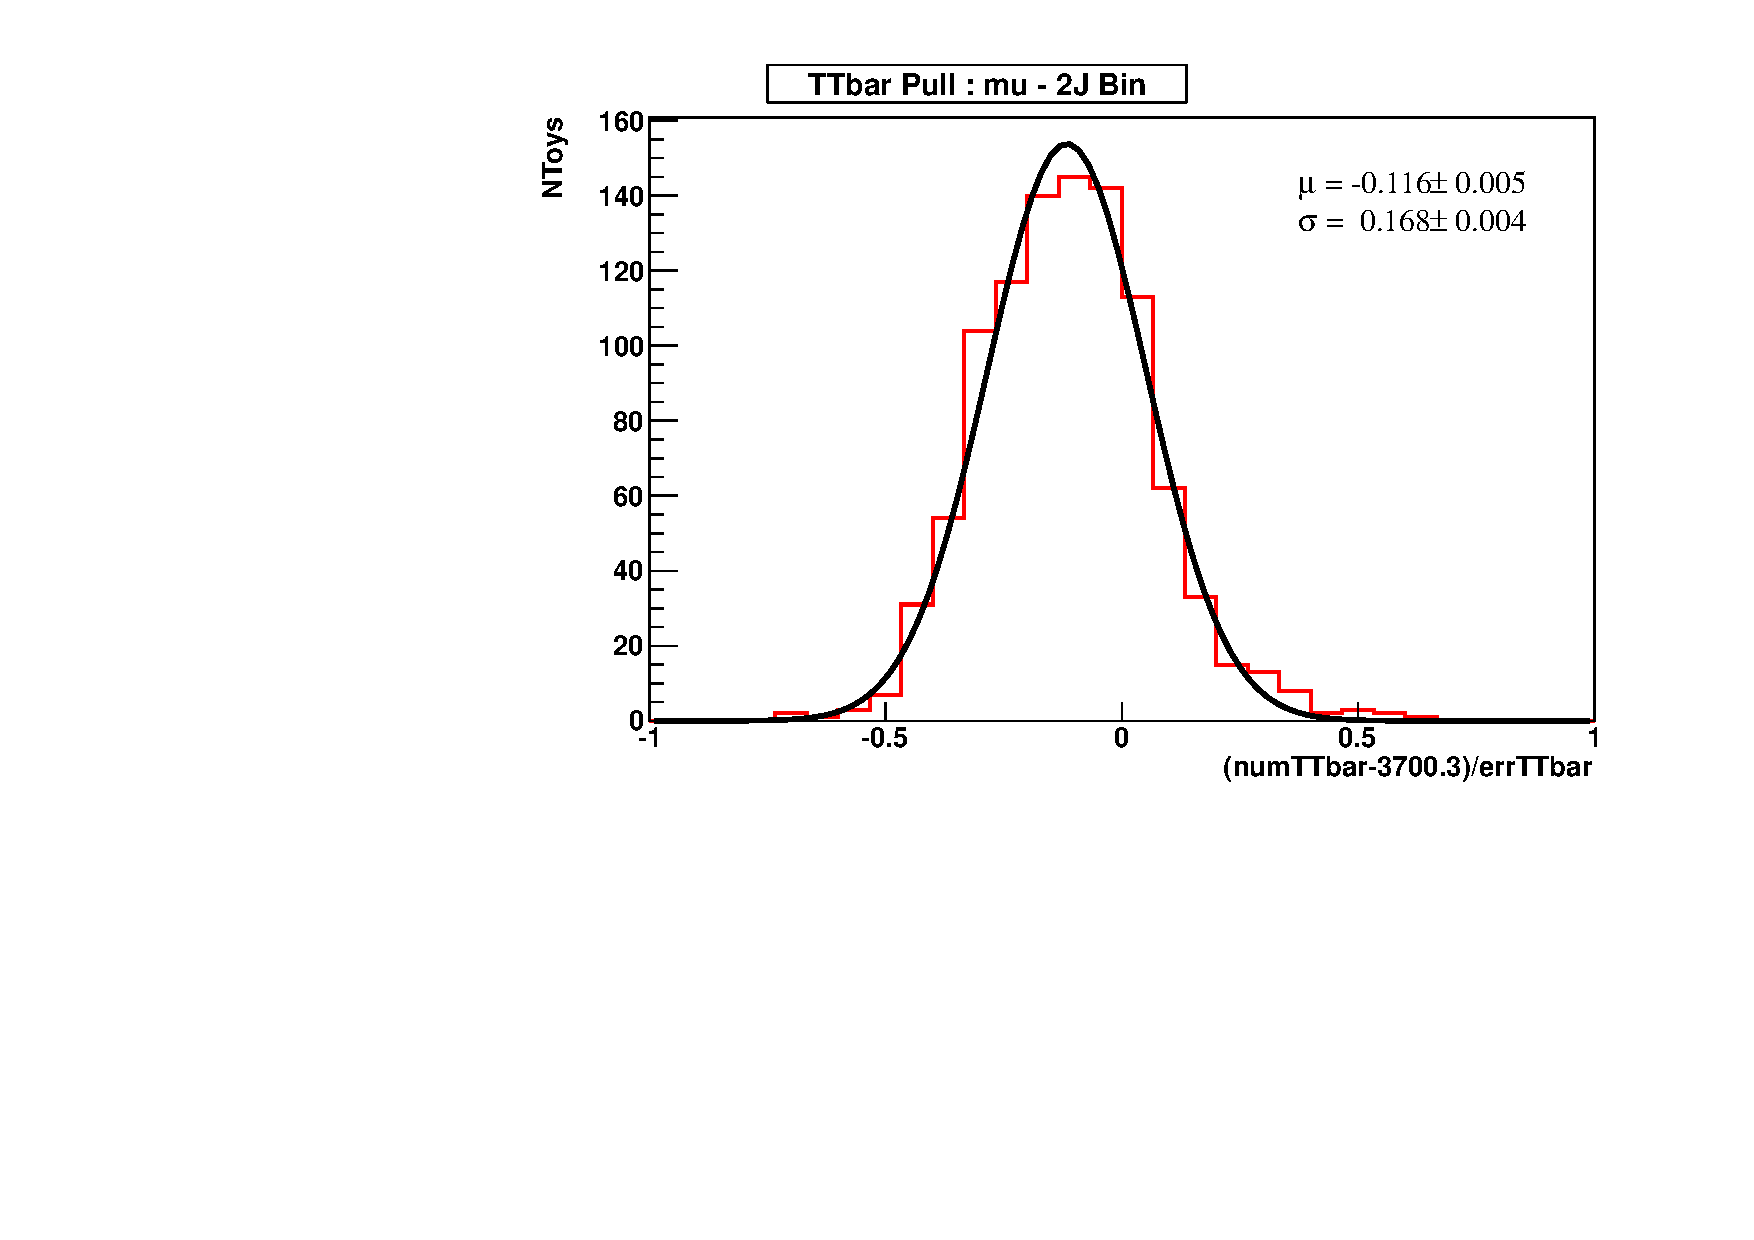
\includegraphics[width=0.48\textwidth]{figs/validation/TTbarPull_Validation_mu_2j.pdf}
\put(-0.80,0.0){(e)} 
\unitlength=0.33\linewidth
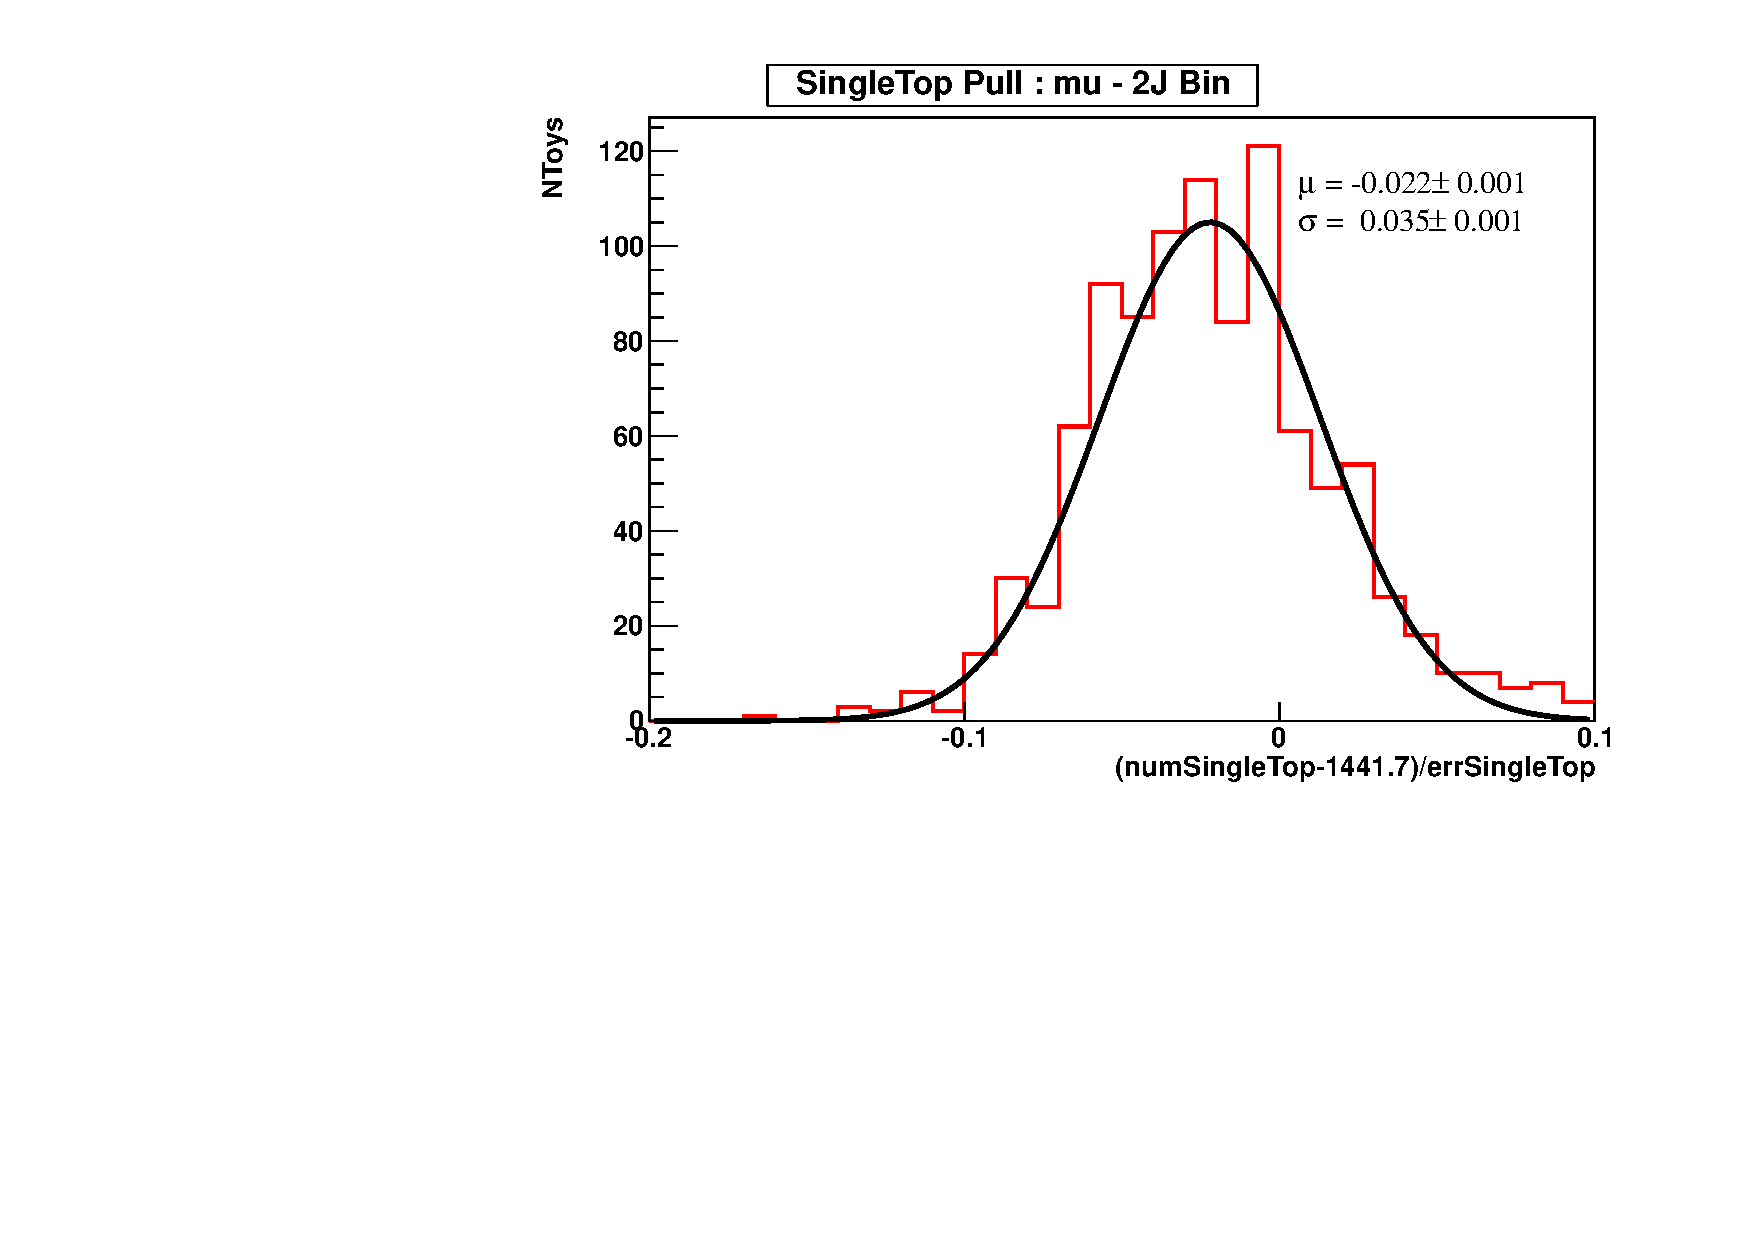
\includegraphics[width=0.48\textwidth]{figs/validation/SingleTopPull_Validation_mu_2j.pdf}
\put(-0.80,0.0){(f)} 
\caption{Fit validation in the 2-jet bin of the muon channel, using 1000 Toy MC datasets. Pull=(Fitted-Expected)/Error for: (a) Diboson, (b) W+jets, (c) Z+jets, (d) QCD, (e) $t\bar{t}$, (f) SingleTop.} 
\label{fig:Validation_Pulls_2j}}
\end{figure}
%%%%%%%
%%%%%%%
\begin{figure}[h!] {\centering
\unitlength=0.33\linewidth
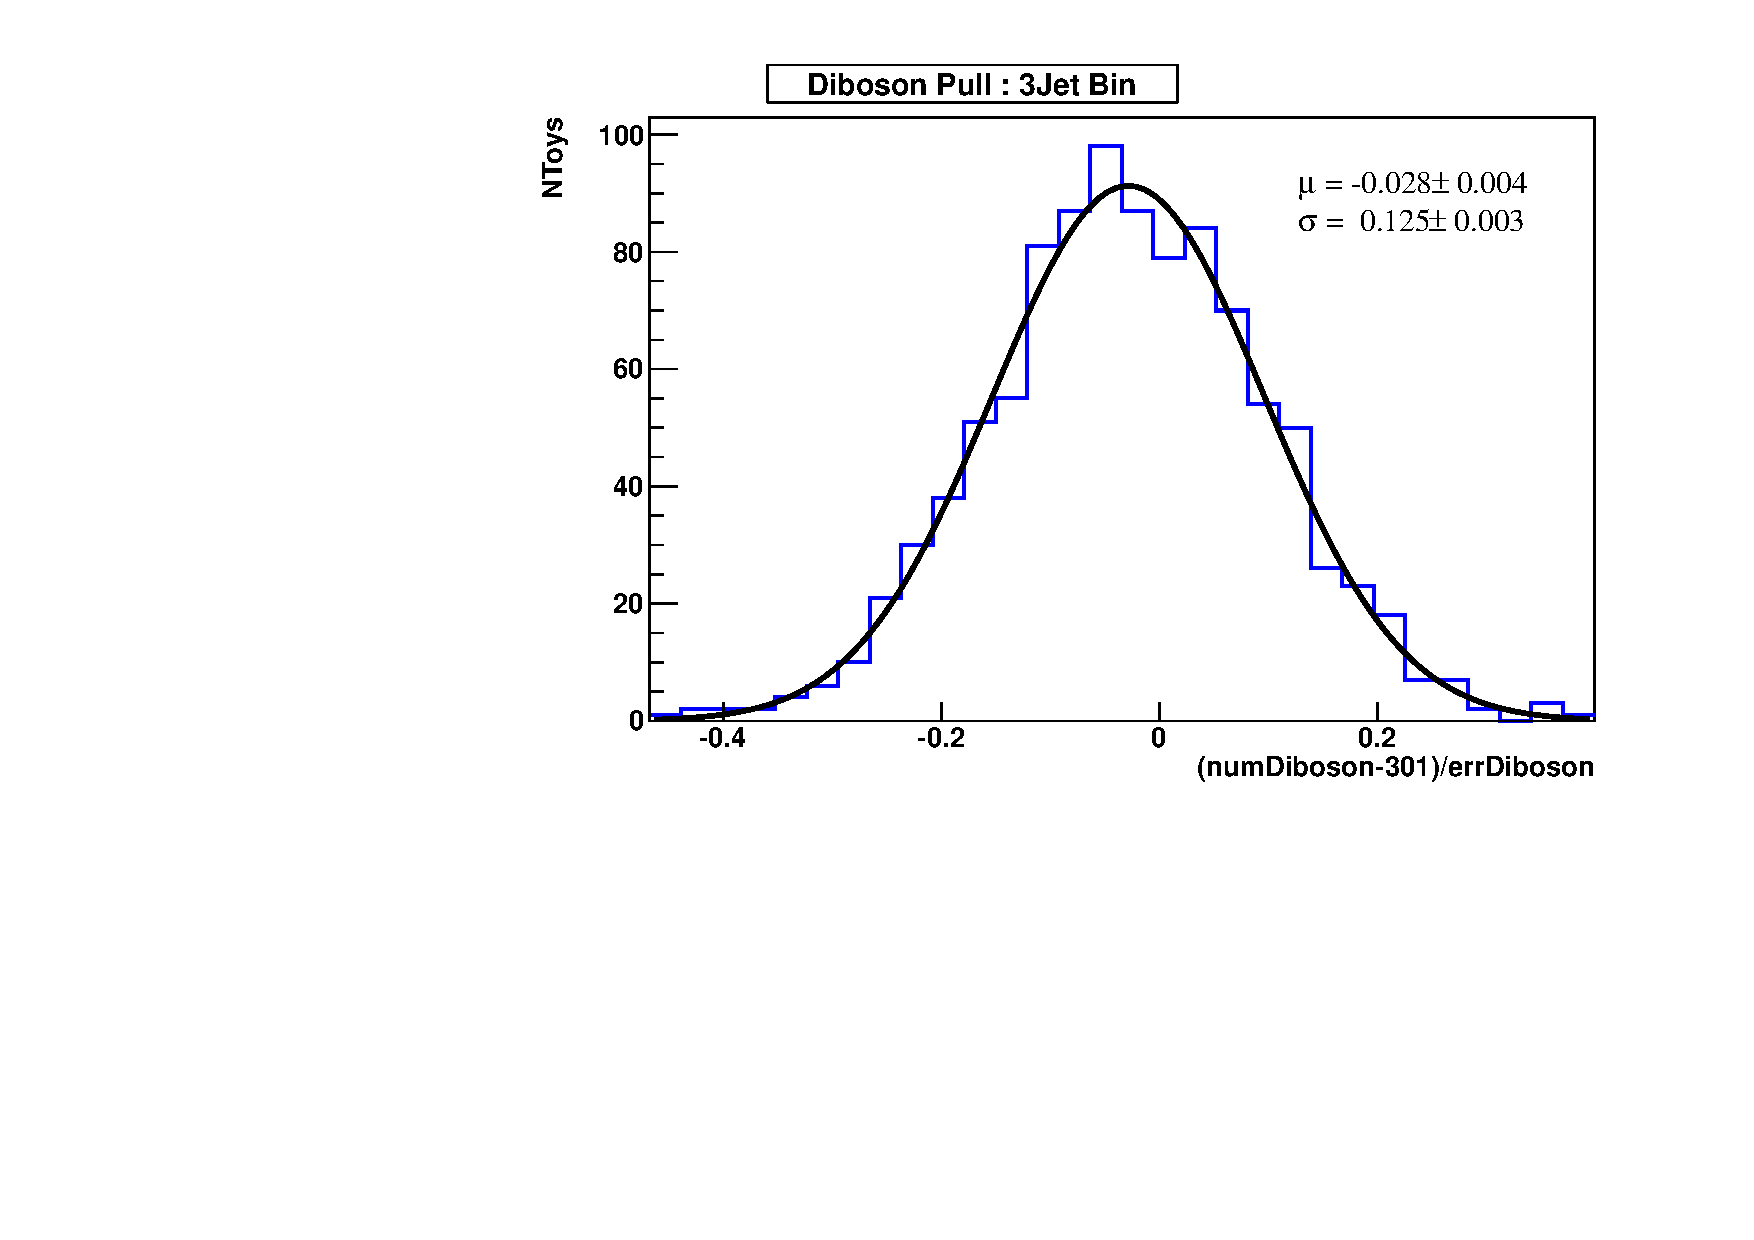
\includegraphics[width=0.48\textwidth]{figs/validation/DibosonPull_Validation_mu_3j.pdf}
\put(-0.80,0.0){(a)} 
\unitlength=0.33\linewidth
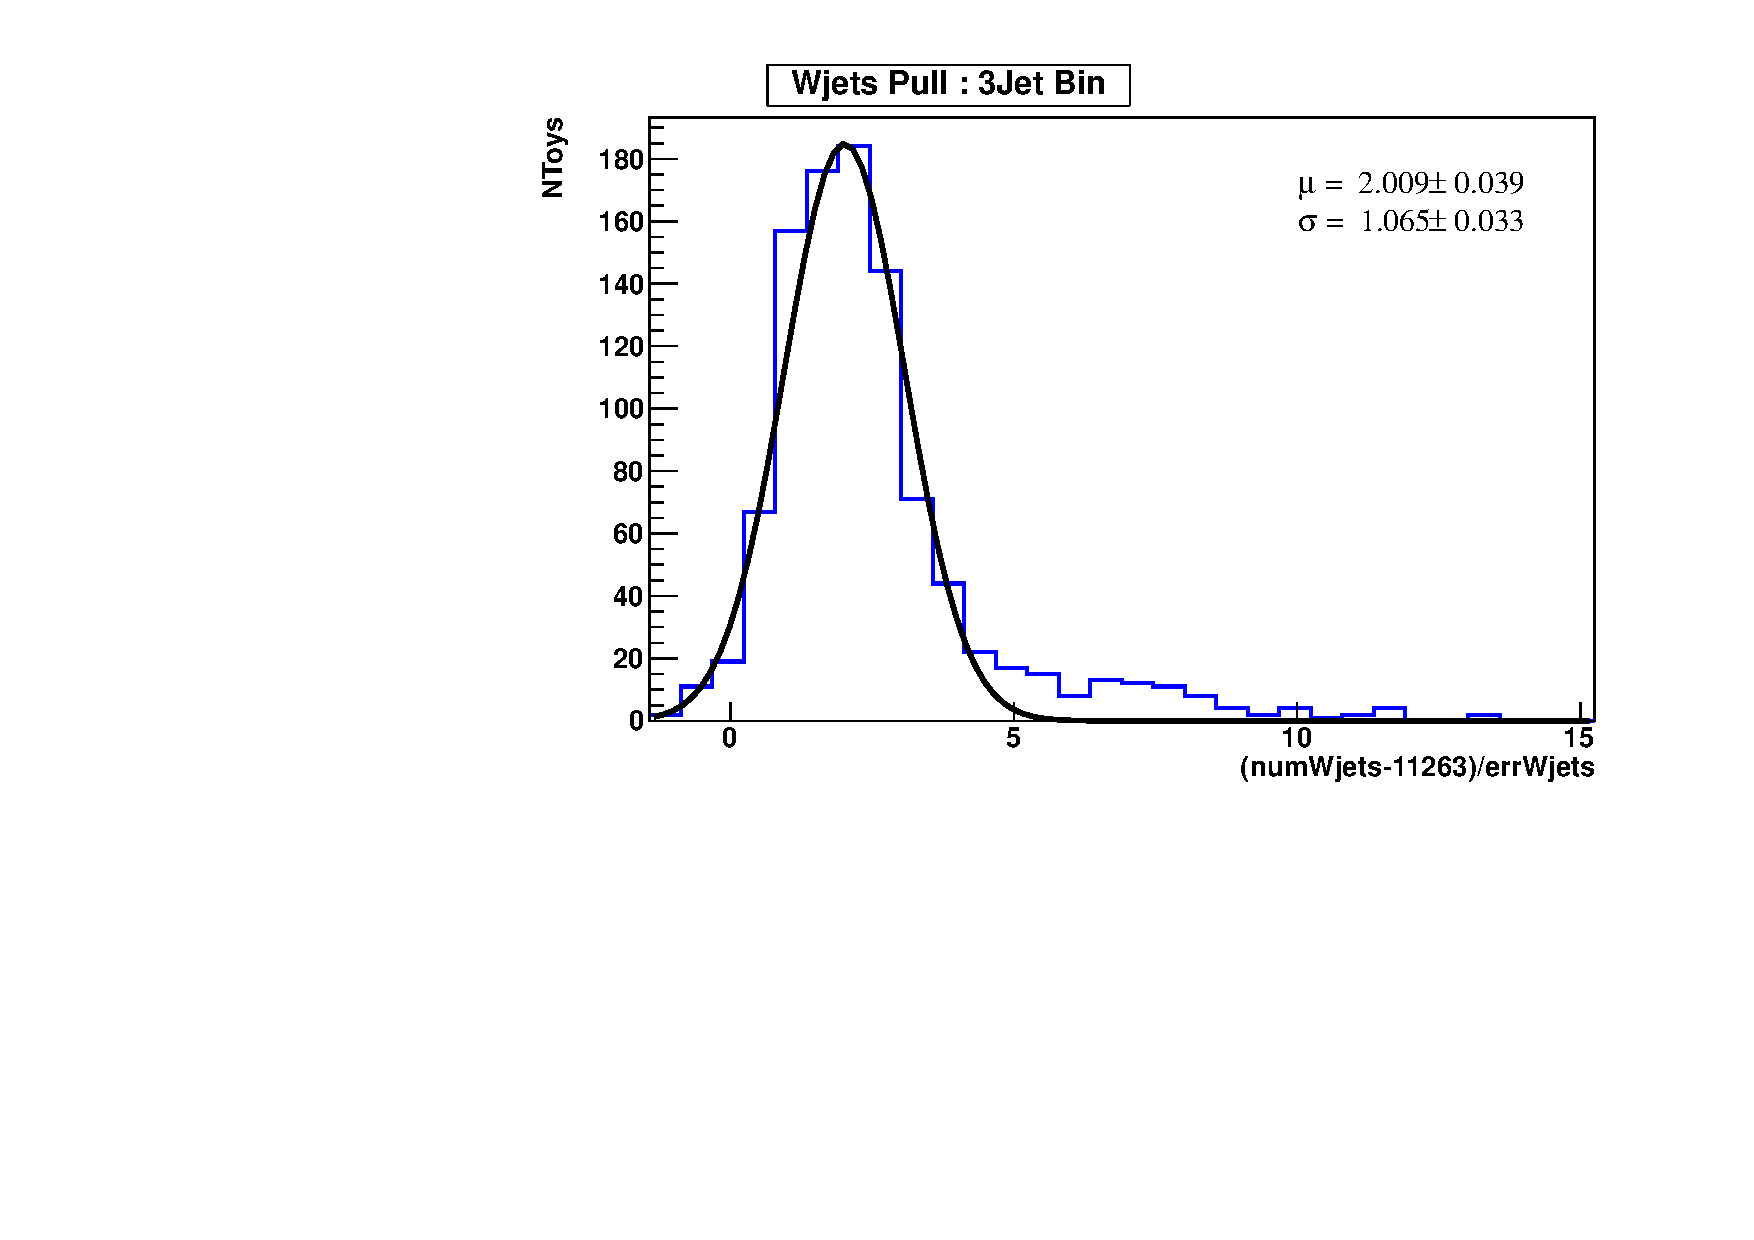
\includegraphics[width=0.48\textwidth]{figs/validation/WjetsPull_Validation_mu_3j.pdf}
\put(-0.80,0.0){(b)} \\
\unitlength=0.33\linewidth
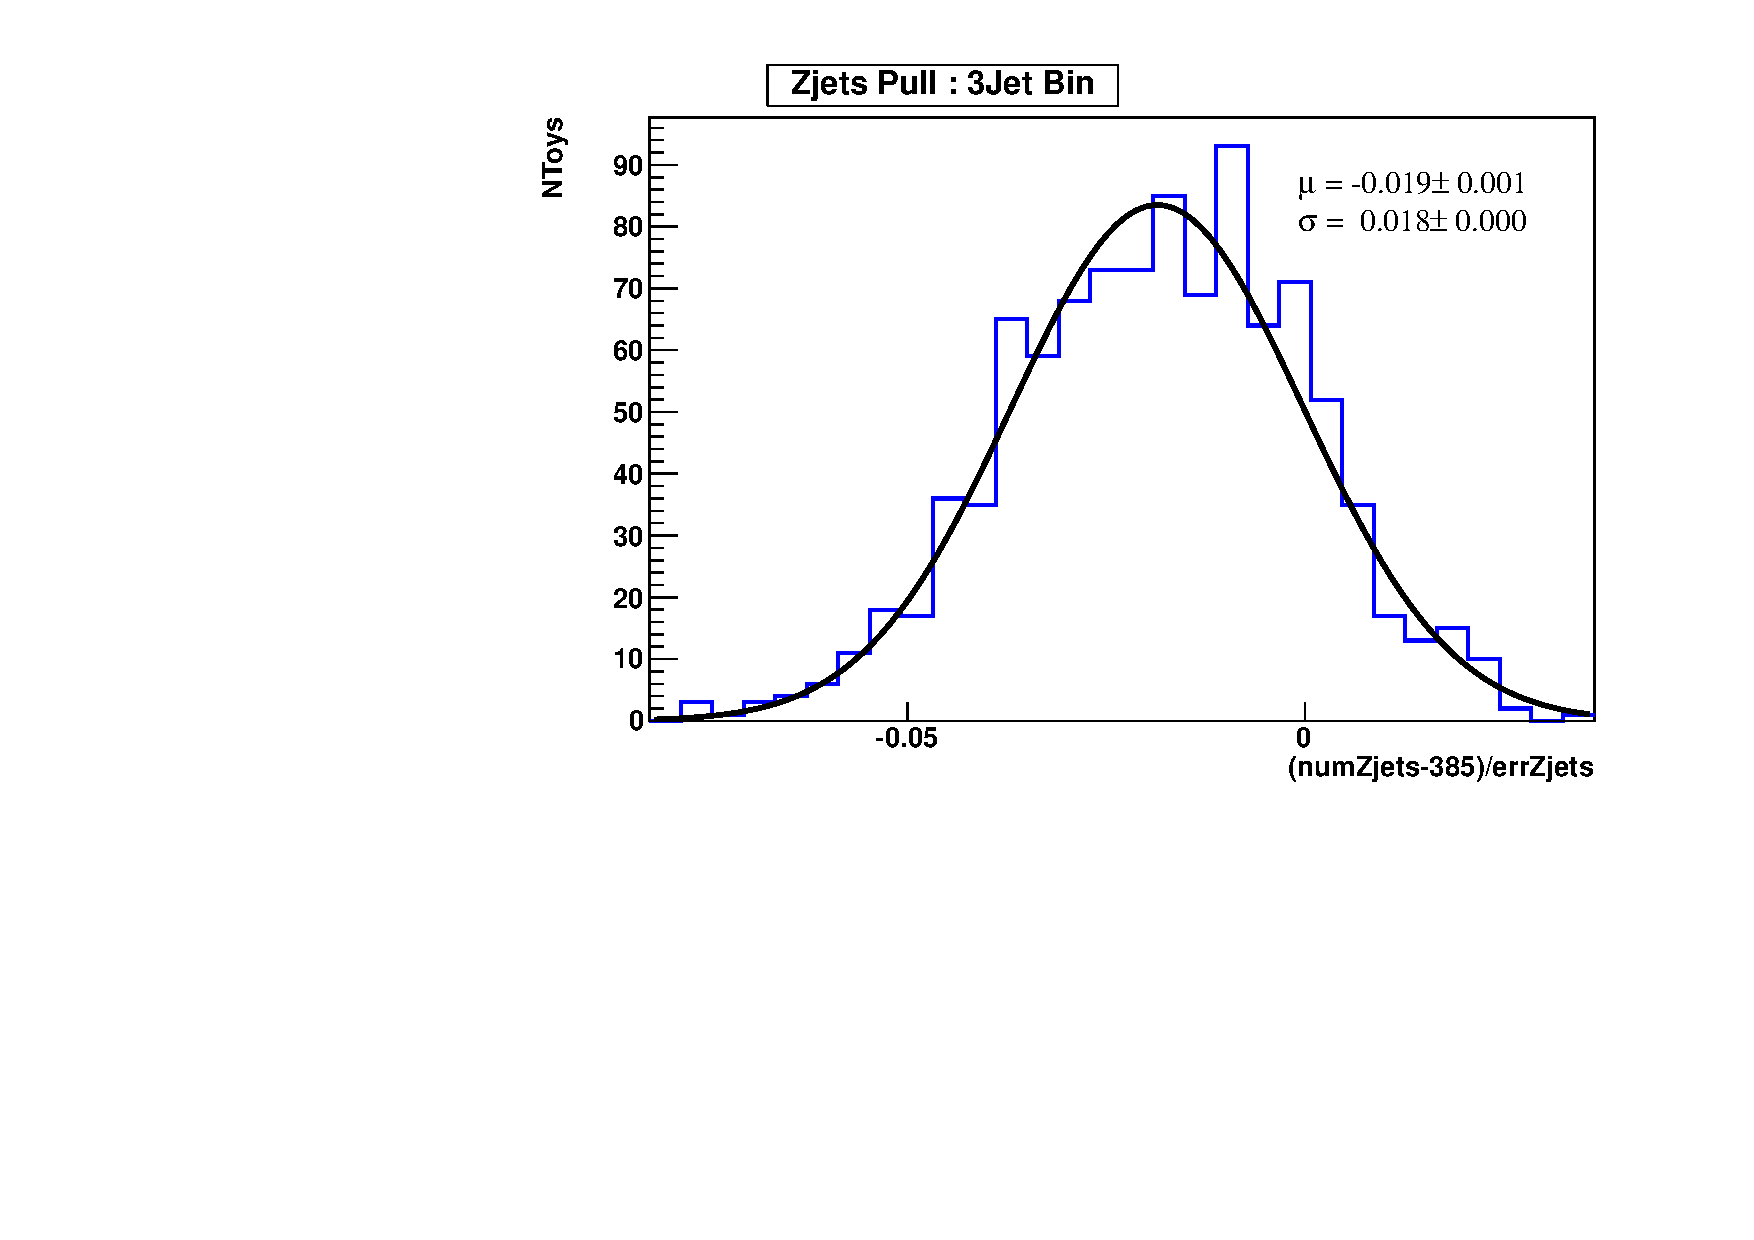
\includegraphics[width=0.48\textwidth]{figs/validation/ZjetsPull_Validation_mu_3j.pdf}
\put(-0.80,0.0){(c)} 
\unitlength=0.33\linewidth
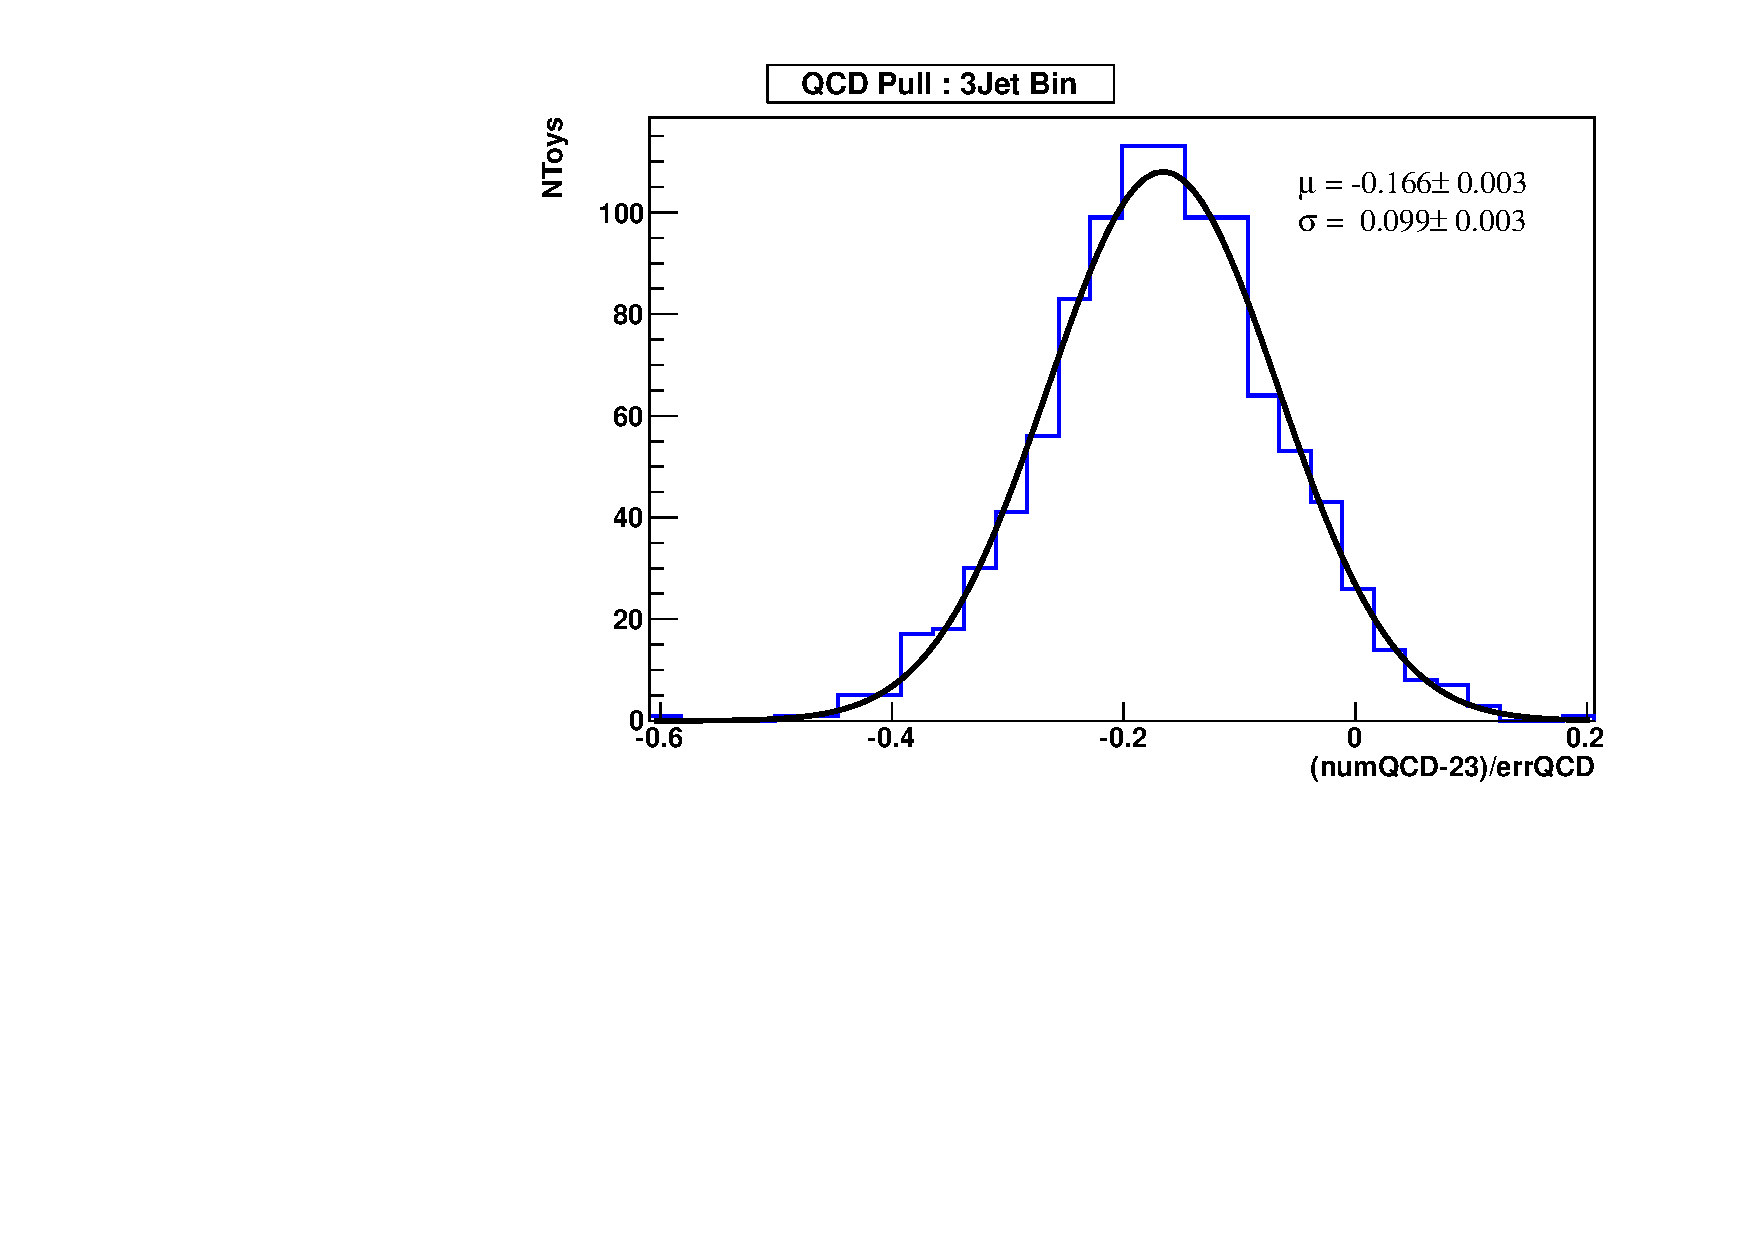
\includegraphics[width=0.48\textwidth]{figs/validation/QCDPull_Validation_mu_3j.pdf}
\put(-0.80,0.0){(d)} \\
\unitlength=0.33\linewidth
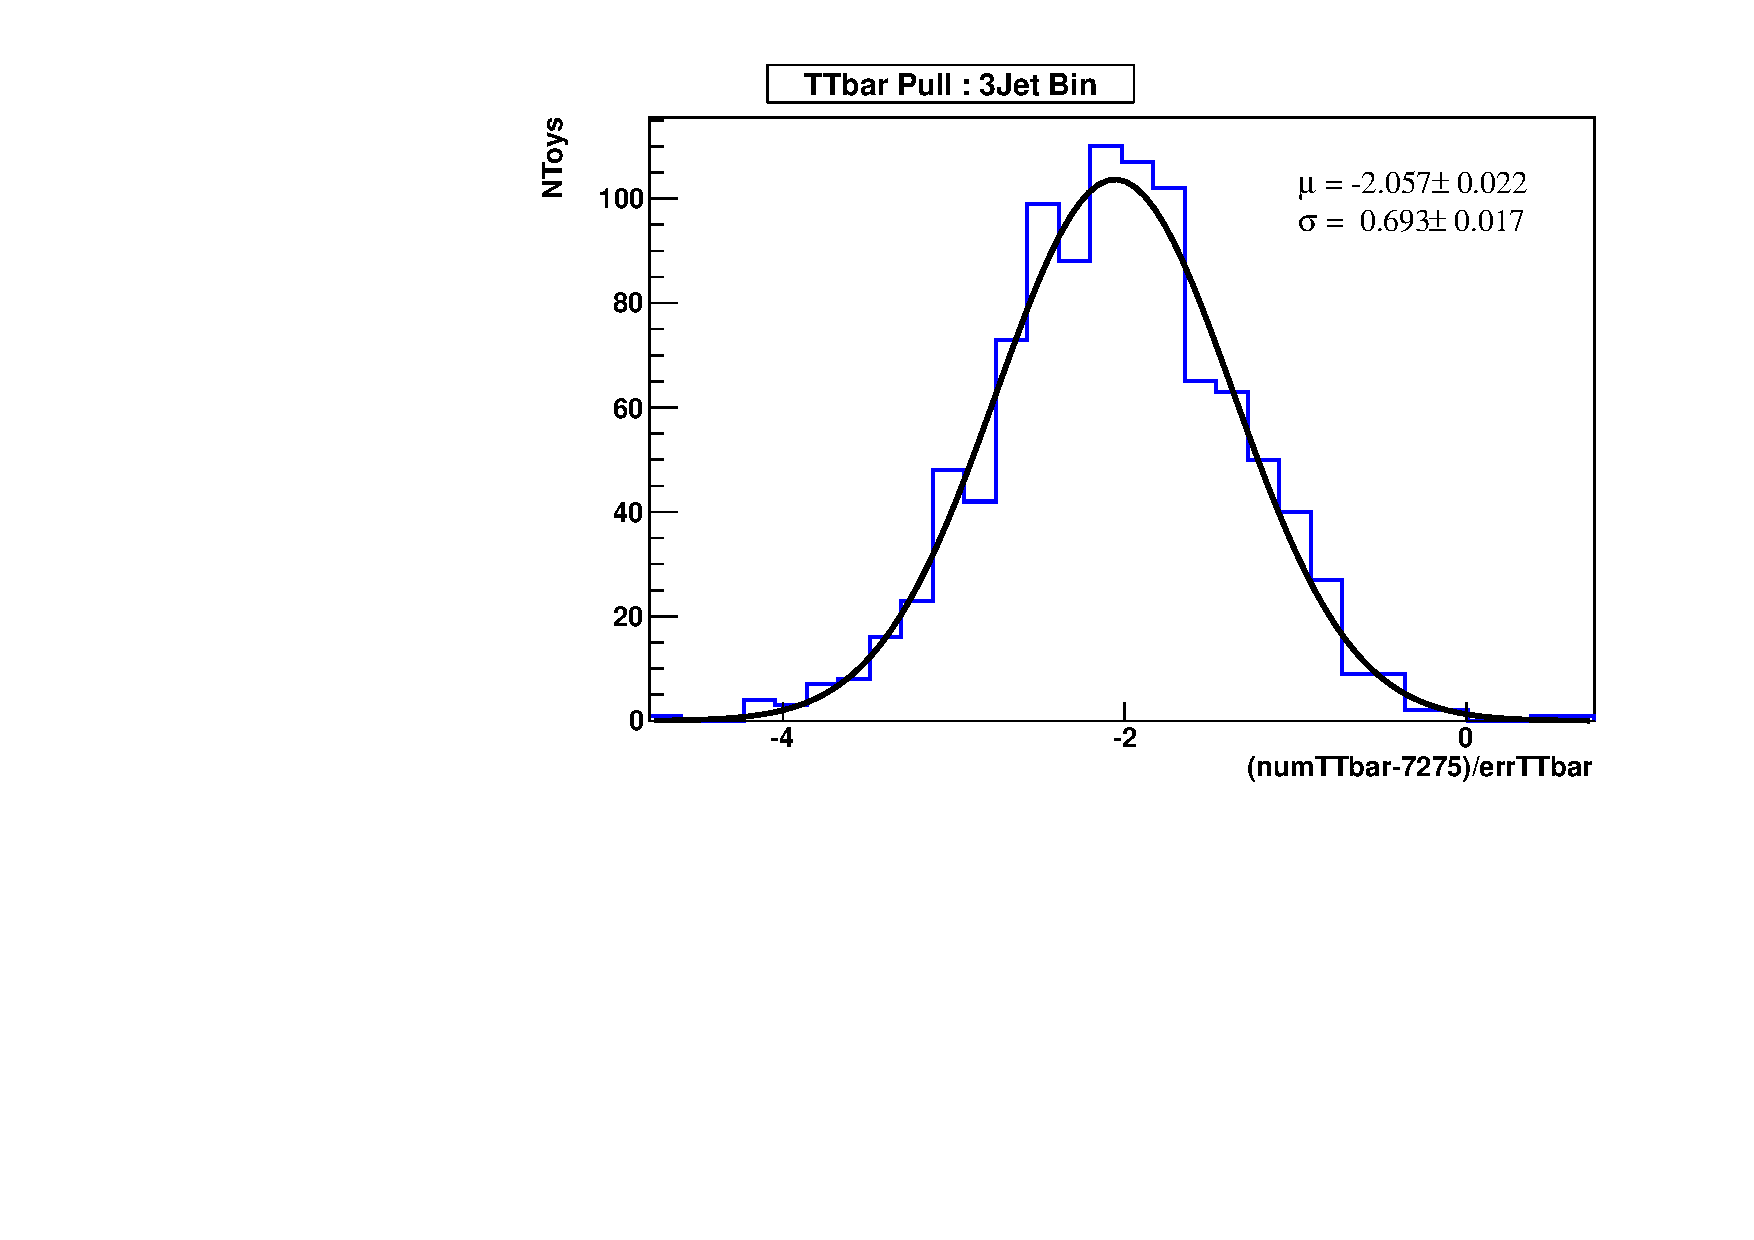
\includegraphics[width=0.48\textwidth]{figs/validation/TTbarPull_Validation_mu_3j.pdf}
\put(-0.80,0.0){(e)} 
\unitlength=0.33\linewidth
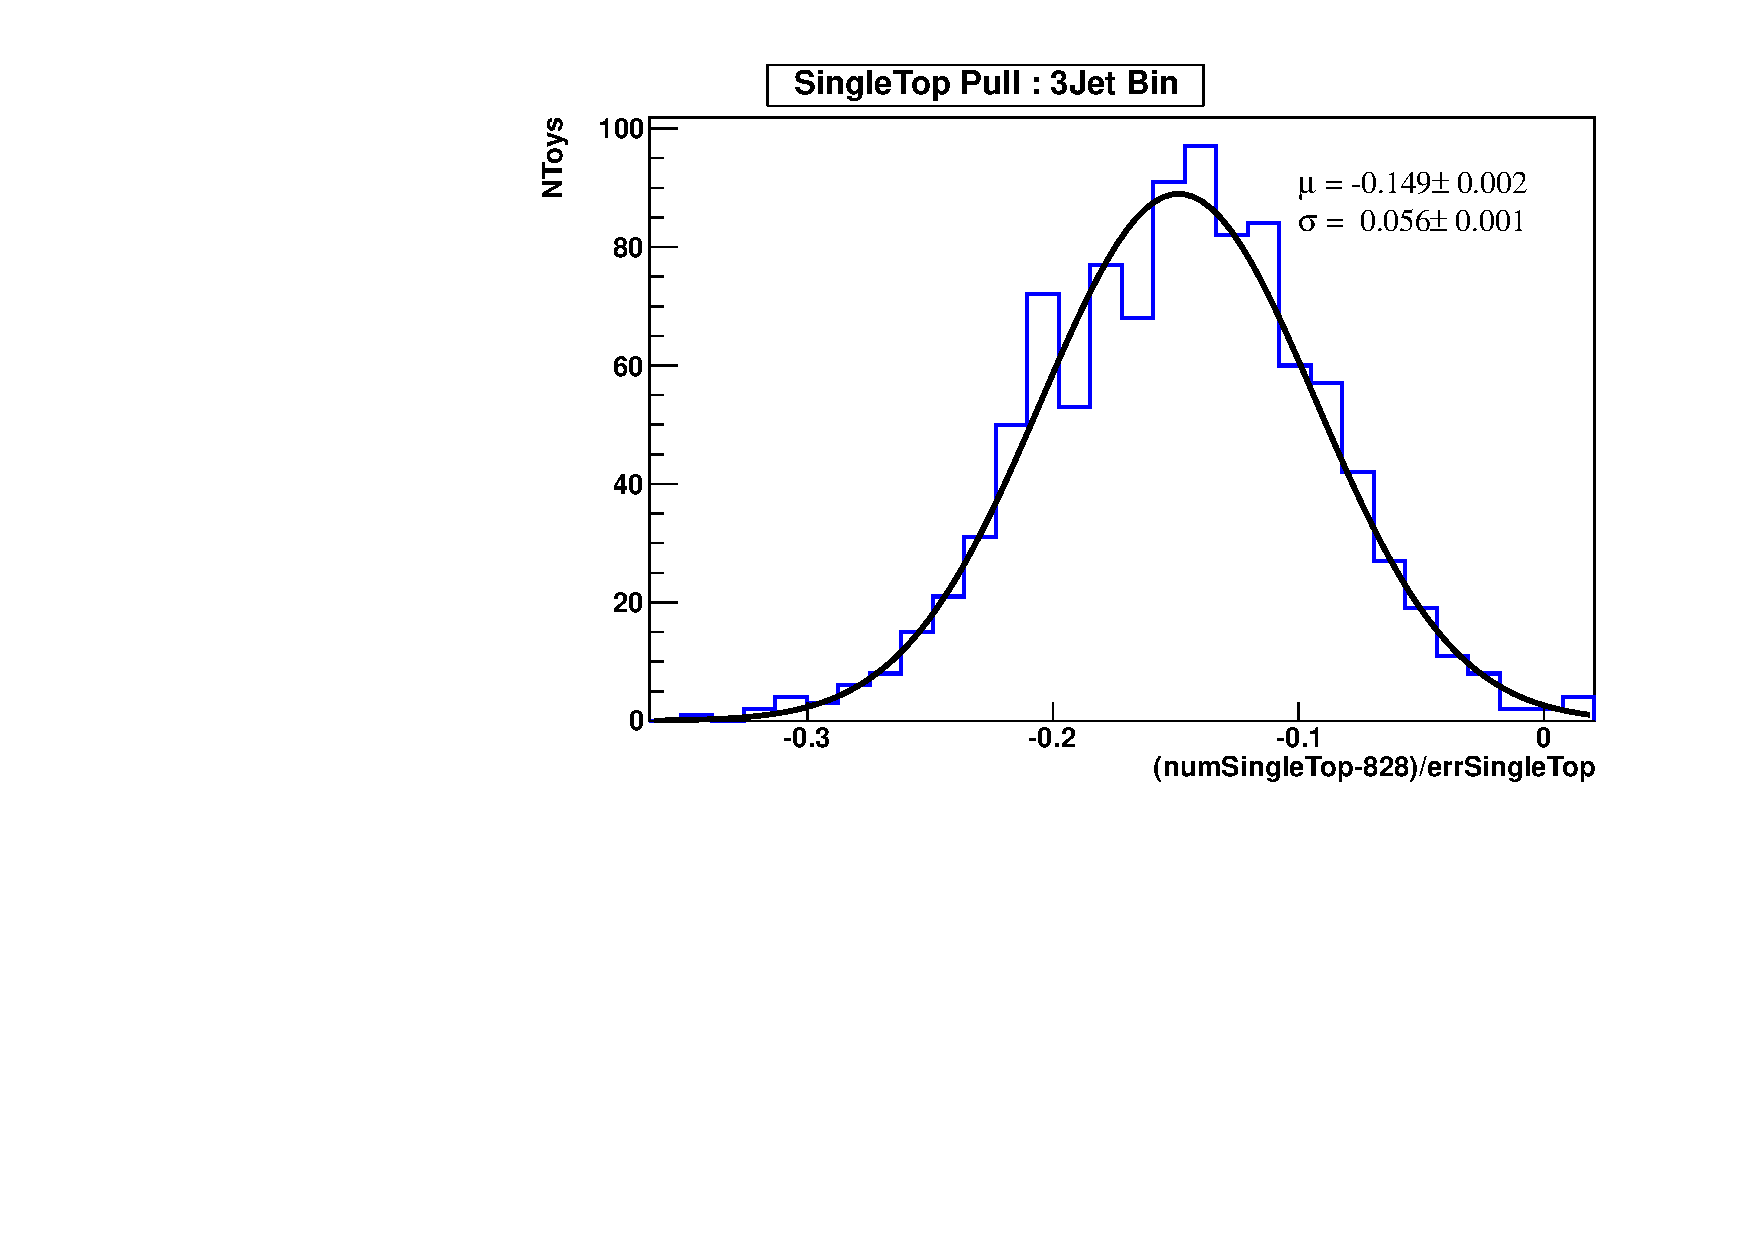
\includegraphics[width=0.48\textwidth]{figs/validation/SingleTopPull_Validation_mu_3j.pdf}
\put(-0.80,0.0){(f)} 
\caption{Fit validation in the 3-jet bin of the muon channel, using 1000 Toy MC datasets. Pull=(Fitted-Expected)/Error for: (a) Diboson, (b) W+jets, (c) Z+jets, (d) QCD, (e) $t\bar{t}$, (f) SingleTop.} 
\label{fig:Validation_Pulls_3j}}
\end{figure}
%%%%%%%
%%%%%%%
\begin{figure}[h!] {\centering
\unitlength=0.33\linewidth
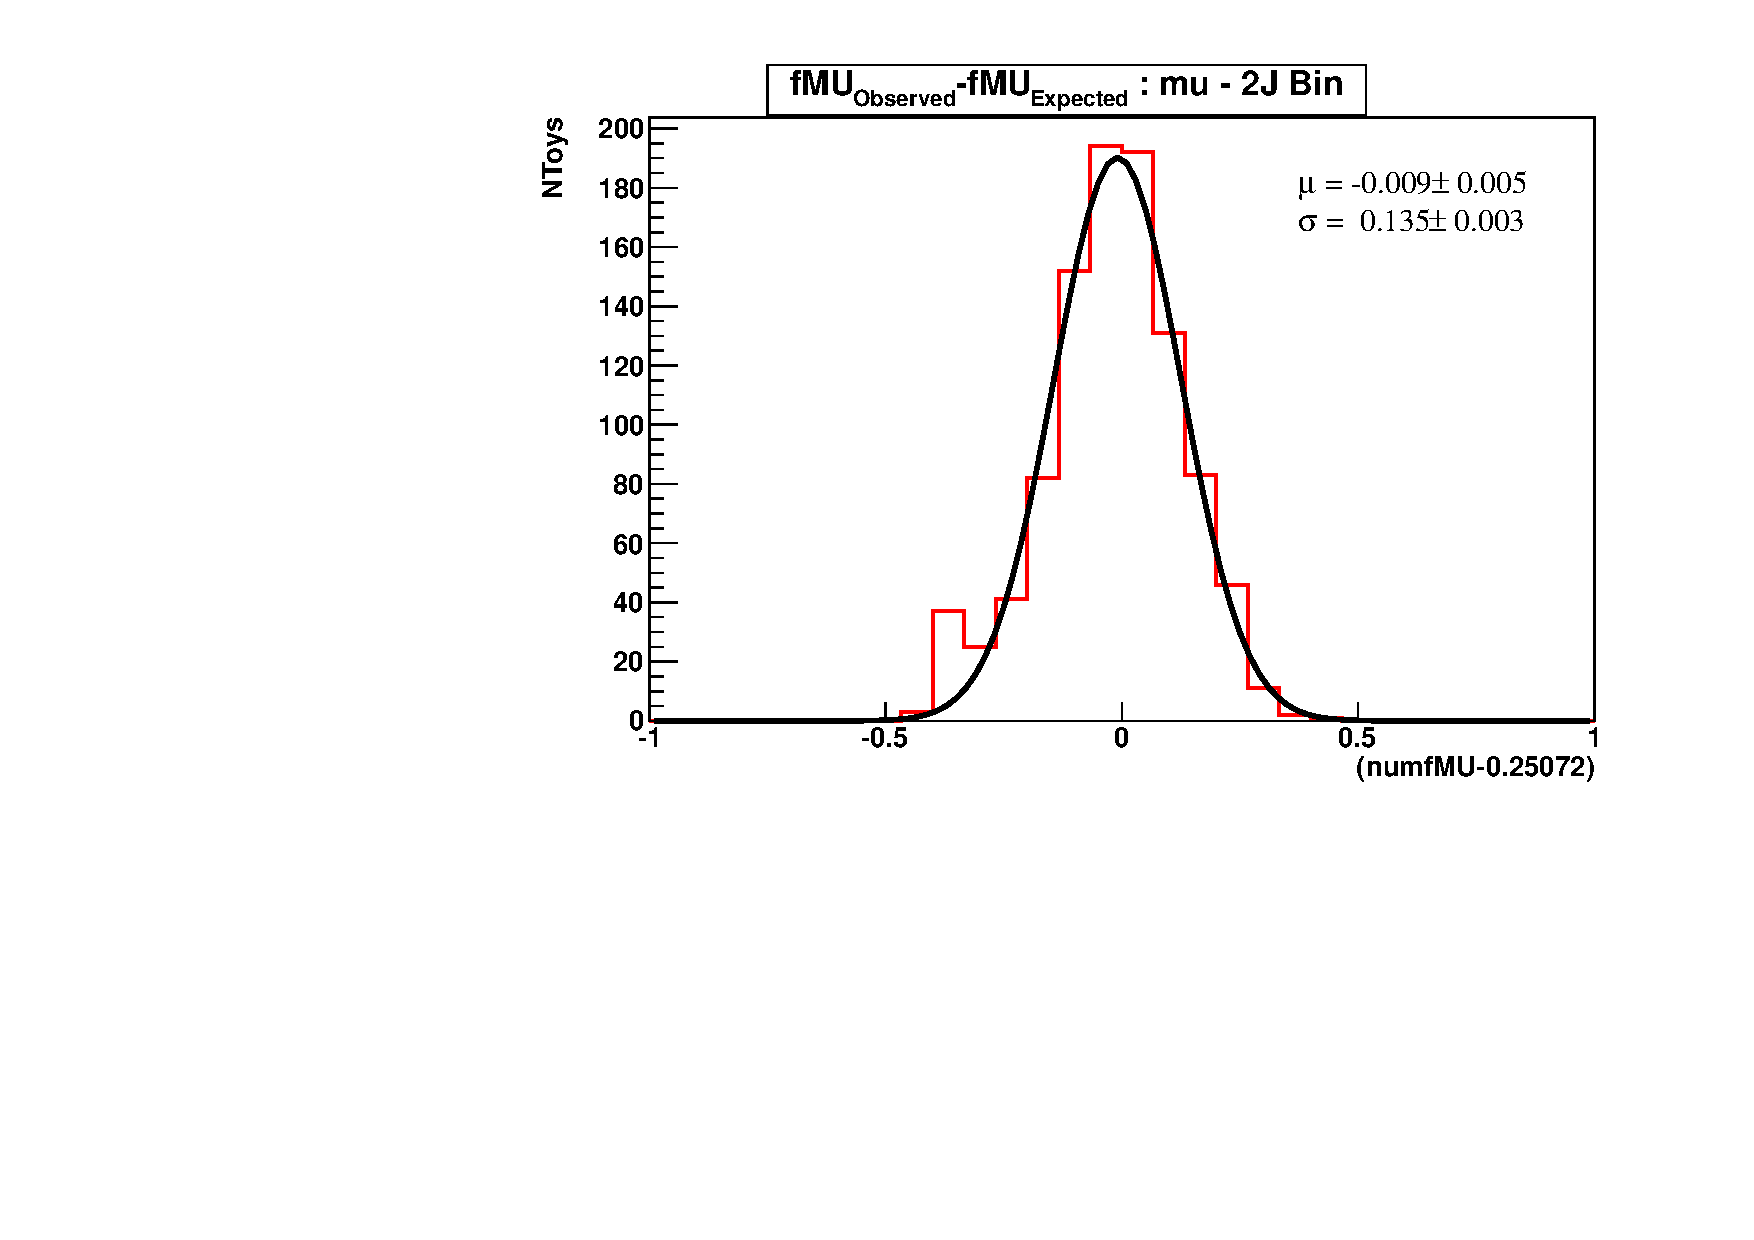
\includegraphics[width=0.48\textwidth]{figs/validation/fMUYield_Validation_mu_2j.pdf}
\put(-0.80,0.0){(a)} 
\unitlength=0.33\linewidth
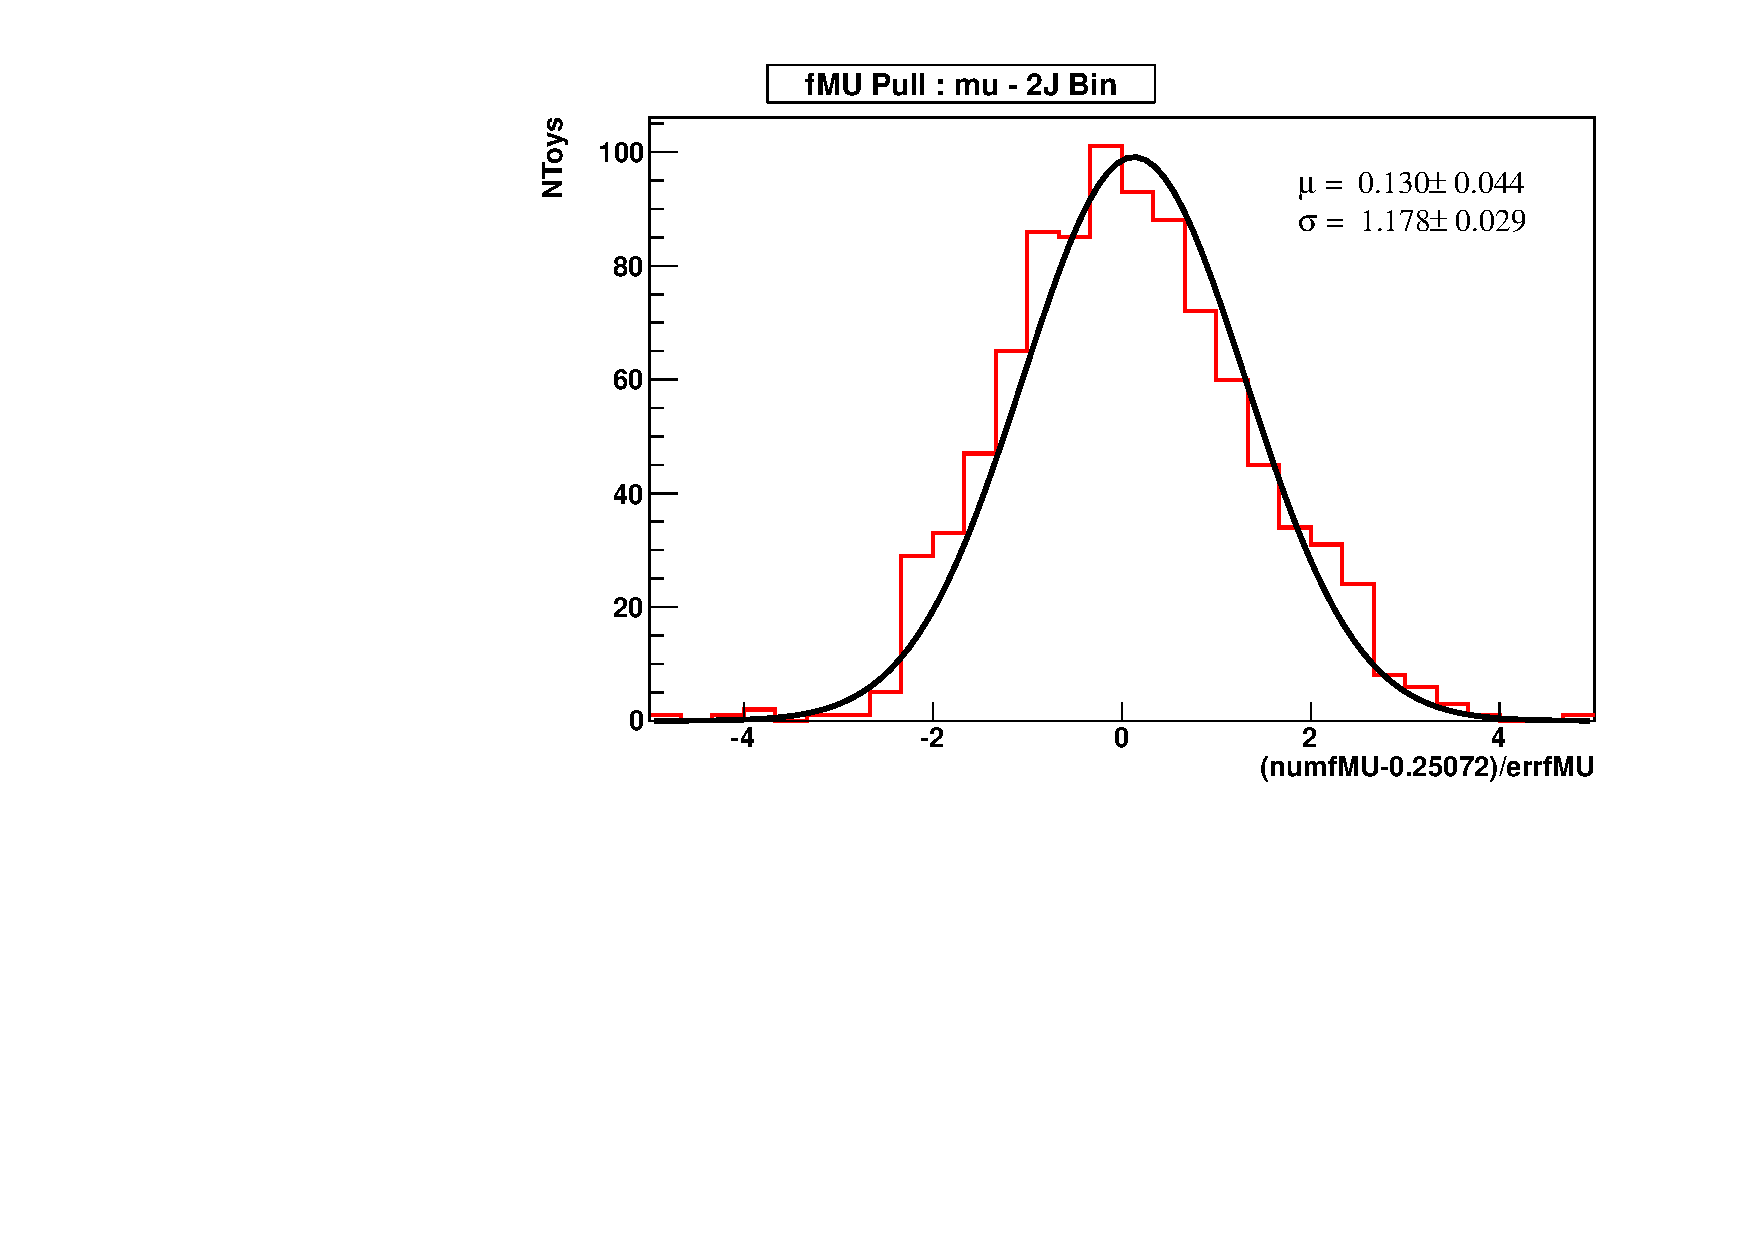
\includegraphics[width=0.48\textwidth]{figs/validation/fMUPull_Validation_mu_2j.pdf}
\put(-0.80,0.0){(b)} \\
\unitlength=0.33\linewidth
\includegraphics[width=0.48\textwidth]{figs/validation/fSUYield_Validation_mu_2j.pdf}
\put(-0.80,0.0){(c)} 
\unitlength=0.33\linewidth
\includegraphics[width=0.48\textwidth]{figs/validation/fSUPull_Validation_mu_2j.pdf}
\put(-0.80,0.0){(d)}
\caption{Fit validation in the 2-jet bin of the muon channel, using 1000 Toy MC datasets. Matching Up Fraction (a) Fitted-Expected (b) Pull distributions; and Scale Up Fraction (c) Fitted-Expected (d) Pull distributions. By convention $fMU<0$ ($fSU<0$) denotes that we are using the Matching Down (Scale Down) sample with the fraction $-fMU$ ($-fSU$).} 
\label{fig:Validation_fMUfSU_2j}}
\end{figure}
%%%%%%%
%%%%%%%
\begin{figure}[h!] {\centering
\unitlength=0.33\linewidth
\includegraphics[width=0.48\textwidth]{figs/validation/fMUYield_Validation_mu_3j.pdf}
\put(-0.80,0.0){(a)} 
\unitlength=0.33\linewidth
\includegraphics[width=0.48\textwidth]{figs/validation/fMUPull_Validation_mu_3j.pdf}
\put(-0.80,0.0){(b)} \\
\unitlength=0.33\linewidth
\includegraphics[width=0.48\textwidth]{figs/validation/fSUYield_Validation_mu_3j.pdf}
\put(-0.80,0.0){(c)} 
\unitlength=0.33\linewidth
\includegraphics[width=0.48\textwidth]{figs/validation/fSUPull_Validation_mu_3j.pdf}
\put(-0.80,0.0){(d)}
\caption{Fit validation in the 3-jet bin of the muon channel, using 1000 Toy MC datasets. Matching Up Fraction (a) Fitted-Expected (b) Pull distributions; and Scale Up Fraction (c) Fitted-Expected (d) Pull distributions. By convention, $fMU<0$ ($fSU<0$) indicates that we are using the Matching Down (Scale Down) sample with the fraction $-fMU$ ($-fSU$).} 
\label{fig:Validation_fMUfSU_3j}}
\end{figure}
%%%%%%%
%%%%%%%
\begin{figure}[h!] {\centering
\unitlength=0.33\linewidth
\includegraphics[width=0.48\textwidth]{figs/validation/ShapeComp_Scale2j.pdf}
\put(-0.80,0.0){(a)} 
\unitlength=0.33\linewidth
\includegraphics[width=0.48\textwidth]{figs/validation/ShapeComp_Scale3j.pdf}
\put(-0.80,0.0){(b)} \\
\unitlength=0.33\linewidth
\includegraphics[width=0.48\textwidth]{figs/validation/ShapeComp_Matching2j.pdf}
\put(-0.80,0.0){(c)} 
\unitlength=0.33\linewidth
\includegraphics[width=0.48\textwidth]{figs/validation/ShapeComp_Matching3j.pdf}
\put(-0.80,0.0){(d)} 
\caption{Comparison between Up and Down shapes for: (a) scale - 2-jet bin, (b) scale - 3-jet bin, (c) matching - 2-jet bin, (d) matching - 3-jet bin.} 
\label{fig:Validation_fMUfSU_ShapeComparisonUpVsDown}}
\end{figure}
%%%%%%%
%%%%%%%
\begin{figure}[h!] {\centering
\unitlength=0.33\linewidth
\includegraphics[width=0.48\textwidth]{figs/validation/TotalYield_Validation_mu_2j.pdf}
\put(-0.80,0.0){(a)} 
\unitlength=0.33\linewidth
\includegraphics[width=0.48\textwidth]{figs/validation/TotalPull_Validation_mu_2j.pdf}
\put(-0.80,0.0){(b)} \\
\unitlength=0.33\linewidth
\includegraphics[width=0.48\textwidth]{figs/validation/TotalYield_Validation_mu_3j.pdf}
\put(-0.80,0.0){(c)} 
\unitlength=0.33\linewidth
\includegraphics[width=0.48\textwidth]{figs/validation/TotalPull_Validation_mu_3j.pdf}
\put(-0.80,0.0){(d)}
\caption{Fit validation in the muon channel, using 1000 Toy MC datasets. 2-jet bin (a) Fitted-Expected (b) Pull distributions; and 3-jet bin (c) Fitted-Expected (d) Pull distributions.} 
\label{fig:Validation_Total_YieldsAndPulls}}
\end{figure}
%%%%%%%
%%%%%%%%%%%%%%%%%%%%%%%%%%%%
%%%%%%%%%%%%%%%
\begin{table}[tb]
\begin{center}
\caption{Event yields in the muon channel determined from a likelihood fit to the data, their excpected values and totals corrected by the fit bias. The total uncertainty takes
into account the correlations among individual components, while the region $(123\,\text{GeV} < m_{jj} < 186\,\text{GeV})$ is excluded from the fit.}
 \label{table:FitTotalsAndComparisons_mu} 
 \begin{tabular} {l  c  c c c }
   \hline \hline
   Bin                  &    2 Jets      && 3 Jets & \\  \hline
                        &    Predicted           &  Extracted           &  Predicted         &  Extracted \\  \hline
   W+jets               &  60408    &  58919$\pm$530     &  16143    &  13069$\pm$366  \\
   Dibosons             &  1178     &  1236$\pm$114      &  326      &  333$\pm$32  \\
   $t\bar{t}$           &  4470     &  4570$\pm$307      &  7732     &  9049$\pm$382  \\
   Single top           &  1746     &  1765$\pm$87       &  997      &  1001$\pm$50  \\
   Drell-Yan+jets       &  1834     &  1837$\pm$79       &  560      &  561$\pm$24  \\
   Multijet             &  110      &  29$\pm$284        &  0        &  0.0   \\
   \hline 
   Data/Total Yield     &  67900    &  68294$\pm$307     &  24046    &  24013$\pm$193 \\ 
   \hline
   Corrected Total      &  ---      &  68236$\pm$417     &  ---      &  24049$\pm$286  \\
\hline
\multicolumn{5}{c}{in region $(123\,\text{GeV} < m_{jj} < 186\,\text{GeV})$} \\
\hline
   Data/Total Yield     &  14050    &  14511$\pm$125     &  7751     &  7739$\pm$95 \\
\hline \hline
\end{tabular}
\end{center}
\end{table}
%%%%%%%%%%%%%%%
\begin{table}[tb]
\begin{center}
\caption{Event yields in the electron channel determined from a likelihood fit to the data, their excpected values and totals corrected by the fit bias. The total uncertainty takes
into account the correlations among individual components, while the region $(123\,\text{GeV} < m_{jj} < 186\,\text{GeV})$ is excluded from the fit.}
 \label{table:FitTotalsAndComparisons_el} 
 \begin{tabular} {l  c  c c c }
   \hline \hline
   Bin                  &    2 Jets      && 3 Jets & \\  \hline
                        &    Predicted           &  Extracted           &  Predicted         &  Extracted \\  \hline
   W+jets               &  32189    &  29787$\pm$1153    &  8517     &  8397$\pm$292  \\
   Dibosons             &  658      &  685$\pm$65        &  184      &  184$\pm$18  \\
   $t\bar{t}$           &  2531     &  2556$\pm$174      &  4234     &  4265$\pm$253  \\
   Single top           &  923      &  916$\pm$46        &  524      &  521$\pm$26  \\
   Drell-Yan+jets       &  1061     &  1061$\pm$46       &  364      &  364$\pm$16  \\
   Multijet             &  2584     &  3944$\pm$1133     &  324      &  324$\pm$160   \\
   \hline 
   Data/Total Yield     &  38973    &  38949$\pm$228     &  14145    &  14055$\pm$143 \\ 
   \hline
   Corrected Total      &  ---      &  38916$\pm$309    &  ---      &  14076$\pm$212  \\
\hline
\multicolumn{5}{c}{in region $(123\,\text{GeV} < m_{jj} < 186\,\text{GeV})$} \\
\hline
   Data/Total Yield     &  8023    &  7944$\pm$92    &  4438     &  4347$\pm$70 \\
\hline \hline
\end{tabular}
\end{center}
\end{table}
%%%%%%%%%%%%%%%%%%%%%%%%%%%%%%%%%%%%%%%%%%%%%%%%%%%%%%%%%%%%
\clearpage
%--------------------------------------------------
\subsection{Fit Results With Error}
    We show the fit results with the systematic error included in Figs.~\ref{fig:mjj_2jet_mu_ENP},~\ref{fig:mjj_2jet_el_ENP},~\ref{fig:mjj_3jet_mu_ENP},~\ref{fig:mjj_3jet_el_ENP}. While the exctracted yields do not change from the previous result, the systematic error band includes the corrections from the above validation procedure. In Fig.~\ref{fig:mjj_Combined_ENP} we show the results for the sum of the electrons, muons, 2-jet bin and the 3-jet bin data.


%%%%%%%%%%%%%%%%%%%%
\begin{figure}[h!]
  {\centering
    \includegraphics[width=0.49\textwidth]{figs/mjjfit_withErrandNP/Wjj_Mjj_Muon_2jets_Stacked.pdf}
    \includegraphics[width=0.49\textwidth]{figs/mjjfit_withErrandNP/Wjj_Mjj_Muon_2jets_Stacked_log.pdf}
    \includegraphics[width=0.49\textwidth]{figs/mjjfit_withErrandNP/Wjj_Mjj_Muon_2jets_Subtracted.pdf}
    \includegraphics[width=0.49\textwidth]{figs/mjjfit_withErrandNP/Wjj_Mjj_Muon_2jets_Pull.pdf}
    \caption{Distribution of the dijet invariant mass for the 2-jet events in muon data and Monte Carlo: 
      (upper left) All background components stacked together, 
      (upper right) All background components stacked together on a log scale, (lower left) [Data minus all backgrounds except diboson],  
      (lower right) normalized residual between data and MC. The fit doesn�t include data points in the test region demarcated by the vertical
      lines. The errors on the data points are statistical, but include corrections from the validation procedure.}
    \label{fig:mjj_2jet_mu_ENP}}
\end{figure}
%%%%%%%%%%%%%%%%%%%%
%%%%%%%%%%%%%%%%%%%%
\begin{figure}[h!]
  {\centering
    \includegraphics[width=0.49\textwidth]{figs/mjjfit_withErrandNP/Wjj_Mjj_Electron_2jets_Stacked.pdf}
    \includegraphics[width=0.49\textwidth]{figs/mjjfit_withErrandNP/Wjj_Mjj_Electron_2jets_Stacked_log.pdf}
    \includegraphics[width=0.49\textwidth]{figs/mjjfit_withErrandNP/Wjj_Mjj_Electron_2jets_Subtracted.pdf}
    \includegraphics[width=0.49\textwidth]{figs/mjjfit_withErrandNP/Wjj_Mjj_Electron_2jets_Pull.pdf}

    \caption{Distribution of the dijet invariant mass for the 2-jet events in electron data and Monte Carlo: 
      (upper left) All background components stacked together, 
      (upper right) All background components stacked together on a log scale, (lower left) [Data minus all backgrounds except diboson],  
      (lower right) normalized residual between data and MC. The fit doesn�t include data points in the test region demarcated by the vertical
      lines. The errors on the data points are statistical, but include corrections from the validation procedure.}
    \label{fig:mjj_2jet_el_ENP}}
\end{figure}
%%%%%%%%%%%%%%%%%%%%
%%%%%%%%%%%%%%%%%%%%
\begin{figure}[h!]
  {\centering
    \includegraphics[width=0.49\textwidth]{figs/mjjfit_withErrandNP/Wjj_Mjj_Muon_3jets_Stacked.pdf}
    \includegraphics[width=0.49\textwidth]{figs/mjjfit_withErrandNP/Wjj_Mjj_Muon_3jets_Stacked_log.pdf}
    \includegraphics[width=0.49\textwidth]{figs/mjjfit_withErrandNP/Wjj_Mjj_Muon_3jets_Subtracted.pdf}
    \includegraphics[width=0.49\textwidth]{figs/mjjfit_withErrandNP/Wjj_Mjj_Muon_3jets_Pull.pdf}
    \caption{Distribution of the dijet invariant mass for the 3-jet events in muon data and Monte Carlo: 
      (upper left) All background components stacked together, 
      (upper right) All background components stacked together on a log scale, (lower left) [Data minus all backgrounds except diboson],  
      (lower right) normalized residual between data and MC. The fit doesn�t include data points in the test region demarcated by the vertical
      lines. The errors on the data points are statistical, but include corrections from the validation procedure.}
    \label{fig:mjj_3jet_mu_ENP}}
\end{figure}
%%%%%%%%%%%%%%%%%%%%
%%%%%%%%%%%%%%%%%%%%
\begin{figure}[h!]
  {\centering
    \includegraphics[width=0.49\textwidth]{figs/mjjfit_withErrandNP/Wjj_Mjj_Electron_3jets_Stacked.pdf}
    \includegraphics[width=0.49\textwidth]{figs/mjjfit_withErrandNP/Wjj_Mjj_Electron_3jets_Stacked_log.pdf}
    \includegraphics[width=0.49\textwidth]{figs/mjjfit_withErrandNP/Wjj_Mjj_Electron_3jets_Subtracted.pdf}
    \includegraphics[width=0.49\textwidth]{figs/mjjfit_withErrandNP/Wjj_Mjj_Electron_3jets_Pull.pdf}

    \caption{Distribution of the dijet invariant mass for the 3-jet events in electron data and Monte Carlo: 
      (upper left) All background components stacked together, 
      (upper right) All background components stacked together on a log scale, (lower left) [Data minus all backgrounds except diboson],  
      (lower right) normalized residual between data and MC. The fit doesn�t include data points in the test region demarcated by the vertical
      lines. The errors on the data points are statistical, but include corrections from the validation procedure.}
    \label{fig:mjj_3jet_el_ENP}}
\end{figure}
%%%%%%%%%%%%%%%%%%%%
%%%%%%%%%%%%%%%%%%%%
\begin{figure}[h!]
  {\centering
    \includegraphics[width=0.32\textwidth]{figs/mjjfit_withErrandNP/Mjj_Stacked_combined.pdf}
    \includegraphics[width=0.32\textwidth]{figs/mjjfit_withErrandNP/Mjj_Subtracted_combined.pdf}
    \includegraphics[width=0.32\textwidth]{figs/mjjfit_withErrandNP/Mjj_Pull_combined.pdf}
    \caption{Distribution of the dijet invariant mass for all (i.e. muon 2-jet, electron 2-jet, muon 3-jet and electron 3-jet): 
      (left) All background components stacked together, 
      (center) Data minus all backgrounds except diboson,  
      (right) Normalized residual between data and MC. The fit doesn�t include data points in the test region demarcated by the vertical
      lines. The errors on the data points are statistical, but include corrections from the validation procedure.}
    \label{fig:mjj_Combined_ENP}}
\end{figure}